% globale Parameter (Papierformat, Schriftgroeße, Trennlinien, Doppelseitig)
\documentclass[a4paper, 11pt, headsepline,footsepline,twoside,abstract]{scrbook}


%%% Verwendete Pakete %%%

\usepackage{url}
\usepackage{geometry} % Seitenraender
\usepackage{fancyhdr} % Schoenere Kopf/Fußzeilen
\usepackage[utf8]{inputenc} % Kodierung
\usepackage[ngerman]{babel} % Sprache
\usepackage{graphicx}  % Bildchen
\usepackage{float}  % Bildchen2
\usepackage{setspace} % fuer Zeilenabstand
\usepackage[T1]{fontenc} % fuer Schriftart
%\usepackage{cite} % fuer Zitate
\usepackage[numbers,square]{natbib} % Package für Zitierstil
\usepackage{pgfplots} % Plots
\usepackage[justification=RaggedRight, singlelinecheck=false, margin=1.5cm]{caption}  % huebschere Captions
\usepackage[version=3]{mhchem} % chemische Formeln
\usepackage{booktabs} % schoenere Tabellen
\usepackage{tabulary} % seitenbreite Tabellen
\usepackage{tabularx} % custom-Breite + Anordnung in tabulars
\usepackage{multirow} % s.o.
\usepackage{ifthen} % s.o.
%\usepackage[FIGTOPCAP]{subfigure} % Grafiken nebeneinander darstellen, deprecated
\usepackage[position=top, font=small]{subfig}% s.o.
\usepackage{textcomp} %Euro-Zeichen
\usepackage{siunitx} % Einheiten korrekt anzeigen
%\sisetup{
% locale = DE ,
% per-mode = symbol,
% separate-uncertainty %+- Notation
%}
%\DeclareSIUnit{\masspercent}{m\%}
%\newcommand{\euro}{\,\texteuro\ } %Euro einfuegen

%Schriftart aendern
\newcommand{\changefont}[3]{
\fontfamily{#1} \fontseries{#2} \fontshape{#3} \selectfont}
\changefont{ptm}{m}{n}

% neue modi tabular
\newcolumntype{L}[1]{>{\raggedright\arraybackslash}p{#1}} % linksbündig mit Breitenangabe
\newcolumntype{C}[1]{>{\centering\arraybackslash}p{#1}} % zentriert mit Breitenangabe
\newcolumntype{R}[1]{>{\raggedleft\arraybackslash}p{#1}} % rechtsbündig mit Breitenangabe

% Zeilenabstand 1,5
\onehalfspacing

% weniger breite Seitenraender
\geometry{a4paper,left=28mm,right=28mm, top=32mm, bottom=30mm} 

% Keine Einrueckung bei neuen Absätzen
%\setlength{\parindent}{0pt}
%\setlength{\parskip}{\baselineskip}

% Bissel Tabellenmagie
\newcommand{\forloop}[5][1]{%
\setcounter{#2}{#3}%
\ifthenelse{#4}{#5\addtocounter{#2}{#1}%
\forloop[#1]{#2}{\value{#2}}{#4}{#5}}%
{}}

\newcounter{crcounter}

\newcommand{\compensaterule}[1]{%
\forloop{crcounter}{1}{\value{crcounter} < #1}%
{\vspace*{-\aboverulesep}\vspace*{-\belowrulesep}}}

\newcommand{\multirowbt}[3]{\multirow{#1}{#2}%
{\compensaterule{#1}#3}}

%%% Kopf und Fußzeilendesigns %%%

% normaler Style
\fancypagestyle{normal}
{
\fancyhead[EL]{\thepage}
\fancyhead[ER]{\leftmark}
\fancyhead[OL] {\rightmark}
\fancyhead[OR]{\thepage}
\fancyfoot[OL]{\parbox[b][0.04\columnwidth][t]{0.5\textwidth}{\raggedright Masterarbeit, Christoph Gielisch}}
\fancyfoot[OR]{
	
\includegraphics[height=0.05\columnwidth]{images/IAM_Logo.png}
	%\caption{}
	\label{img:grafik-dummy}
	}
\fancyfoot[OC,EC]{}
\fancyfoot[EL]{
	
\includegraphics[height=0.05\columnwidth]{images/KIT_LOGO.png}
	%\caption{}
	\label{img:grafik-dummy}
	}
\fancyfoot[ER]{\parbox[b][0.04\columnwidth][t]{0.85\textwidth}{\raggedleft  Elektrochemische und NMR-Untersuchung von Festkörperelektrolytkeramiken}}
\renewcommand{\headrulewidth}{0.5pt}
\renewcommand{\footrulewidth}{0.5pt}
}

% Kapitelanfaenge bekommen ein extra Kopf/Fußzeilendesign
\fancypagestyle{plain}
{
\fancyhf{} % clear all header and footer fields
\fancyfoot[R]{\parbox[b][0.04\columnwidth][t]{0.5\textwidth}{\raggedleft \thepage}}
\fancyfoot[L]{
	
\includegraphics[height=0.05\columnwidth]{images/leerpixel.png}
	%\caption{}
	\label{img:grafik-dummy}
	}
\renewcommand{\headrulewidth}{0pt}
\renewcommand{\footrulewidth}{0.5pt}
}

% Die Inhaltsangabe auch
\fancypagestyle{toc}
{
\fancyhf{} % clear all header and footer fields
\fancyfoot[OR]{\parbox[b][0.04\columnwidth][t]{0.5\textwidth}{\raggedleft \thepage}}
\fancyfoot[OL]{
	
\includegraphics[height=0.05\columnwidth]{images/leerpixel.png}
	%\caption{}
	\label{img:grafik-dummy}
	}
\fancyfoot[EL]{\parbox[b][0.04\columnwidth][t]{0.5\textwidth}{\raggedright \thepage}}
\fancyfoot[ER]{
	
\includegraphics[height=0.05\columnwidth]{images/leerpixel.png}
	%\caption{}
	\label{img:grafik-dummy}
	}
\renewcommand{\headrulewidth}{0pt}
\renewcommand{\footrulewidth}{0.5pt}
}

% Festlegung Art der Zitierung
%\bibliographystyle{unsrtdin}

%%%%%%%%%%%%%%%%%%% hier beginnt das Dokument %%%%%%%%%%%%%%%%%%%%
\begin{document}

\thispagestyle{empty}
\begin{center}
%\Large{Karlsruher Institut für Technologie}\\
\end{center}

\begin{figure}
	\centering
	
\includegraphics[width=0.5\columnwidth]{images/KIT_LOGO.png}
	%\caption{}
	\label{img:grafik-dummy}
\end{figure}

\begin{center}
\textbf{\huge{ Elektrochemische und kern\-spin\-resonanz- spek\-tros\-ko\-pische Untersuchung von\\[0.4cm]Festkörperelektrolytkeramiken}}
\end{center}
\begin{center}
\textbf{\Large{}}
\end{center}
\begin{center}
\large{Von der Fakultät für Wirtschaftswissenschaften des \\ Karlsruher Instituts für Technologie genehmigte }
\end{center}
\begin{verbatim}

\end{verbatim}
\begin{center}
\textbf{\LARGE{Masterarbeit}}
\end{center}
\begin{center}
\textbf{\Large{Nr. XYZ}}\\
am
\end{center}
\begin{center}
\textbf{\Large{Institut für Angewandte Materialien - Keramische Werkstoffe und Technologien (IAM-KWT)}}
\end{center}
\begin{center}
von
\end{center}
\begin{center}
\Large{Christoph Gielisch}
\end{center}
\begin{verbatim}
\end{verbatim}
\begin{center}
Eingereicht am 30. September 2015
\end{center}
\begin{center}
\textbf{Referent:} \\ Prof. Dr-Ing. Volker Schulze \\
\textbf{Koreferent:} \\ Prof. Dr. Michael J. Hoffmann\\
\textbf{Betreuer:} \\ Dr. Claudia Bucharsky \\ 
Dr.-Ing. Günter Schell \\
\end{center}
\newpage
\cleardoubleemptypage
% Eidesstattliche Erklärung
\setcounter{page}{1}
\pagenumbering{Roman}
\textbf{\Large{Eidesstattliche Erklärung}}
\\\\
Hiermit erkläre ich, diese Arbeit selbstständig und ohne fremde Hilfe verfasst zu haben. Es wurden nur die in der Arbeit ausdrücklich benannten Quellen und Hilfsmittel benutzt. Wörtlich oder sinngemäß übernommenes Gedankengut ist als solches gekennzeichnet.
\\\\
Karlsruhe, den 30.09.2015
\\\\
\\\\
\\
(Christoph Gielisch) 
 
\newpage

% Eidesstattliche Erklärung2
%\setcounter{page}{1}
%\pagenumbering{Roman}
\hspace{20mm} \\
\textbf{\Large{Zusammenfassung}}
\\\\
TBD
\\\\
\textbf{\Large{Abstract}}
\\\\
TBD
% Inhaltsverzeichnis
%\KOMAoption{open}{left} 
\pagestyle{toc}
\renewcommand*{\chapterpagestyle}{toc} % Die erste Seite des TOC ist auch ein Kapitelanfang
\tableofcontents
\KOMAoption{open}{right} 
\newpage
\cleardoubleemptypage
\pagestyle{normal}
\renewcommand*{\chapterpagestyle}{plain}
\setcounter{page}{1}
\pagenumbering{arabic}
\chapter{Einleitung}
Batterien nehmen in unserem Leben einen immer höheren Stellenwert ein. Sie kommen in nahezu allen mobilen elektrischen Geräten zum Einsatz. Die im Zuge des Klimaschutzes zunehmende Dekarboniserung von Wirtschaft und Gesellschaft erfordert außerdem, dass bisher mittels fossiler Brennstoffe betriebene Geräte und Maschinen in Zukunft elektrisch betrieben werden. Ein Beispiel ist hier die großflächige Einführung von Elektroautomobilen. Aber auch zur Speicherung von volatil erzeugter Energie, beispielsweise bei Wind- und Sonnenenergie, sind leistungsfähige Batterien nötig.
\\\\
Die vorliegende Arbeit betrachtet die Einsatzmöglichkeit von speziellen Keramiken als Festkörperelektrolyt in Batterien. Sie untersucht dabei insbesondere das elektrochemische Verhalten verschiedener Keramiken. Diese werden als Kathodenmaterial in eine Batterietestzelle verbaut. Mit den Ergebnissen unterschiedlicher Messungen wie der zyklischen Voltametrie und der Impedanzspektroskopie werden dann Rückschlüsse auf die Eignung als Festkörperelektrolyt gezogen. Desweiteren wird ein Messsystem für in-situ-Kernspinresonanzspektroskopie konstruiert und getestet. Mit diesem können noch genauere Aussagen über die Art und Weise der Reaktion und Diffusion des Lithiums mit möglichen Festkörperelektrolyten getroffen werden.
\section{Motivation}
Eine Batterie mit einem Festkörperelektrolyten bietet gleich mehrere Vorteile gegenüber der herkömmlichen Flüssigelektrolyt-Batterie. Der Flüssigelektrolyt moderner Lithiumbatterien besteht zumeist aus einem organischem Lösungsmittel und darin gelösten Lithiumsalzen \cite{xu2004nonaqueous}. Diese sind jedoch nicht stabil gegenüber der Luftfeuchtigkeit und reagieren unter der Bildung von ätzenden Substanzen wie Flusssäure ab. Dies ist neben der Unsicherheit beim Versagen der Batterie ebenso auch ein Problem bei der industriellen Großproduktion. Diese kann nur mit großen Anlagen zur Trocknung der Luft erfolgen. Ein Festkörperelektrolyt könnte so gestaltet werden, dass dieser stabil gegenüber der Luftfeuchtigkeit und dem Sauerstoff der Luft ist.
\\\\
Ein weiteres Problem der aktuellen Flüssigelektrolyten ist deren beschränkte Stabilität gegenüber elektrischen Spannungen. Handelsübliche Flüssigelektrolyte sind lediglich bis zu einer Spannung von maximal 5V stabil \cite{tarascon1994new}. Es existieren jedoch Hochvoltelektroden, die von höheren Spannungen profitieren würden. Festkörperelektrolyte könnten diesen Mangel beheben.
\section{Zielsetzung}
\begin{figure}
	\centering
	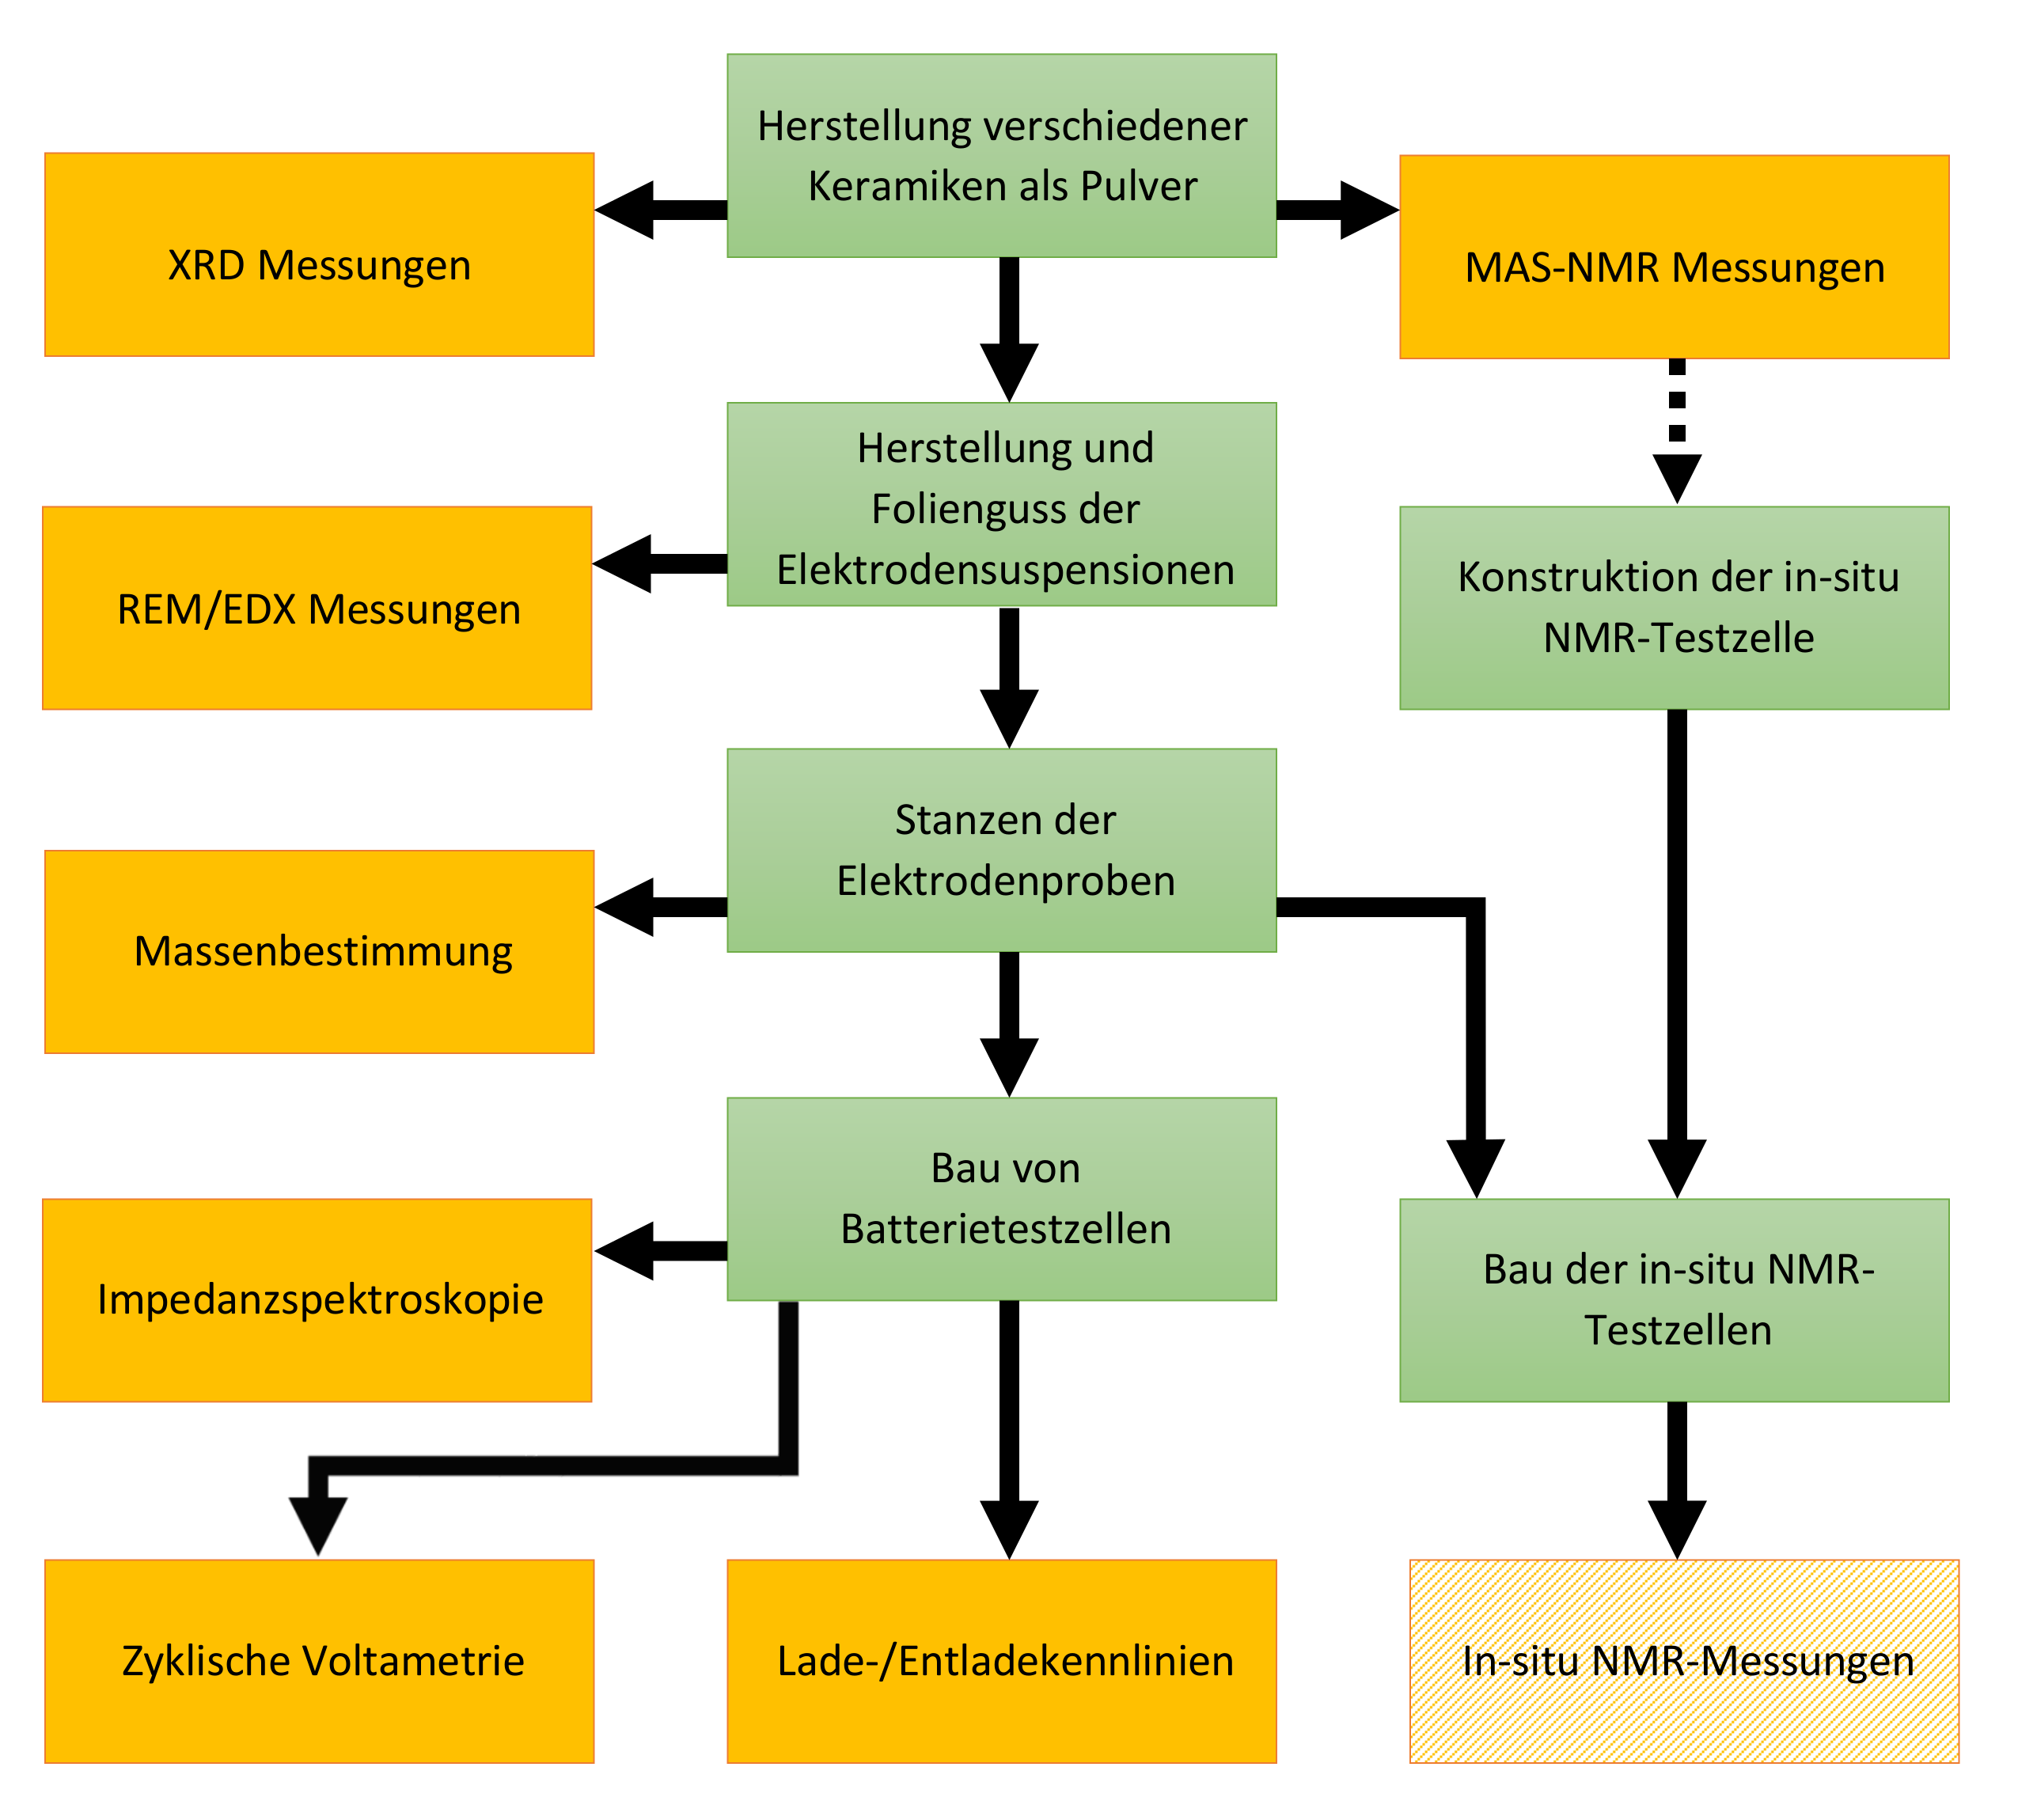
\includegraphics[width=1.0\columnwidth]{images/Flowchart_Masterarbeit2.png}
	\caption{Übersicht über die Probenpräperation (grün), den Messsystemaufbau (blau) und die Messungen (orange) der vorliegenden Arbeit}
	\label{Flowchart_Masterarbeit}
\end{figure}
Ziel der vorliegenden Arbeit ist es, verschiedene Keramiken für den Einsatz als Festkörperelektrolyt zu analysieren. Die Abbildung \ref{Flowchart_Masterarbeit} bietet eine Übersicht über alle dabei zum Einsatz kommenden Schritte. Als Ausgangspunkt dienen hierbei die Materialien \ce{LiLaTiO3} (LLTO) sowie \ce{Li_(_1_+_x_)Al_xTi_(_2_-_x_)(PO4)3} (LATP), die in der Literatur bereits eine ausreichend gute Lithiumleitfähigkeit nachweisen konnten \cite{tatsumisago2013recent}. Die Keramiken sollen in Pulverform, als Elektrodenfolie und im Gefüge Elektrode-Elektrolyt hergestellt werden. Die hergestellten Pulver sollen mittels Röntendiffraktometrie (XRD) und Feststoff-Kernspinspektroskopie (MAS-NMR) untersucht werden. Die gegossenen Elektrodenfolien werden mittel Rasterelektronenmikroskop (REM) genauer charakterisiert. Anschließend werden aus ihnen Batterietestzellen gebaut, welche mittels zyklischer Voltametrie und Impedanzspektroskopie elektrochemisch untersucht werden. Für die Messung von in-situ-NMR-Daten muss sowohl der Lithium-Probenkopf des NMR-Spektrometers angepasst, als auch eine eigene Testzelle konstruiert und gebaut werden.
\section{Aufbau der Arbeit}
Im ersten Kapitel wird die Arbeit motiviert sowie eine Zielsetzung formuliert. Anschließend werden die nötigen Grundlagen für die durchzuführenden Experimente beschrieben. Das dritte Kapitel beschreibt die Konstruktion der in-situ-NMR-Batterietestzelle. Im vierten Kapitel wird die Probenpräperation geschildert. Die erzielten Ergebnisse werden im fünften Kapitel dargestellt und im sechsten Kapitel diskutiert. Das siebte Kapitel bietet eine kurze Zusammenfassung sowie einen Ausblick in die Zukunft.
\chapter{Grundlagen}
Im folgenden Kapitel werden die Grundlagen für die im Rahmen der Arbeit stattgefundenen Experimente gelegt. Dafür wird im ersten Teil der Aufbau und die Elektrochemie sowie die Materialauswahl von Batteriezellen beschrieben. Anschließend werden die in dieser Arbeit untersuchten Keramiken vorgestellt. Zuletzt folgt eine Schilderung der physikalischen Grundlagen sowie des grundsätzlichen Aufbaus eines Kernspinresonanzspektroskops.
\section{Prinzip und Funktionsweise von Batteriezellen}
\begin{figure}
	\centering
	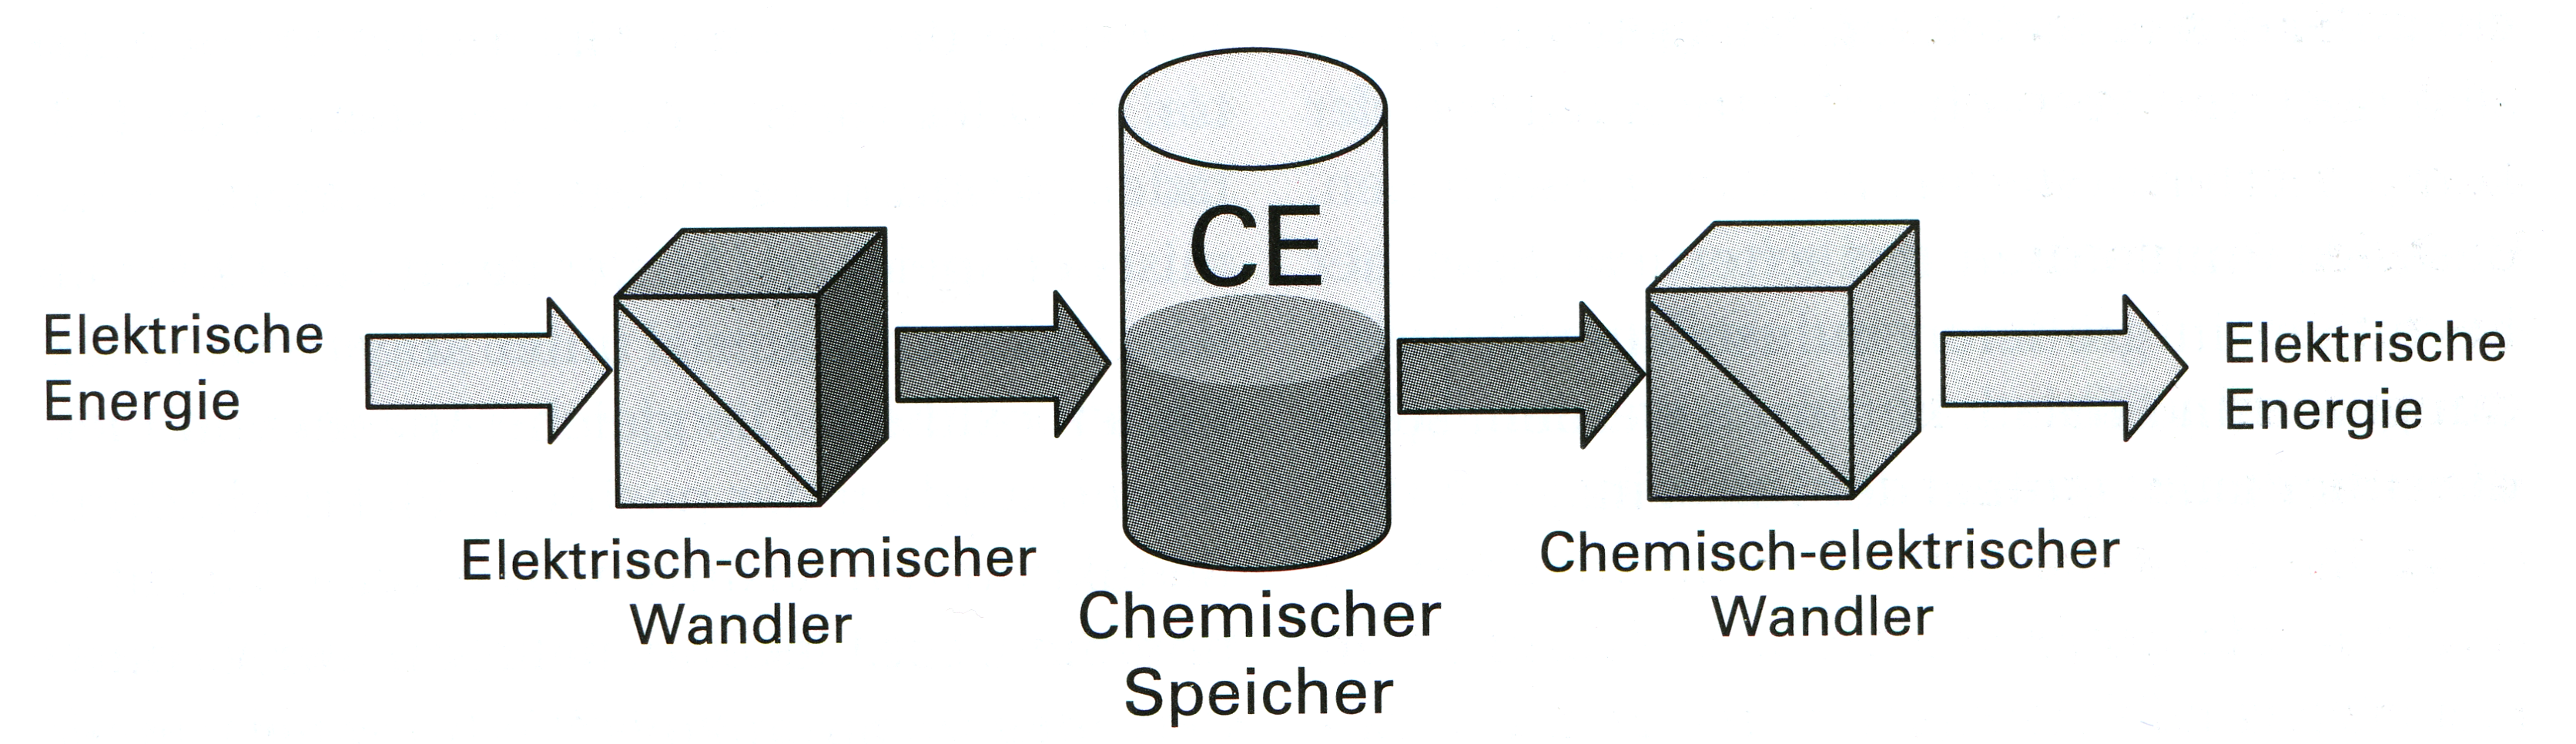
\includegraphics[width=1.0\columnwidth]{images/Prinzipieller_Aufbau.png}
	\caption{Prinzip einer sekundären Zelle \cite{jossen_2006}}
	\label{Prinzip_Zelle}
\end{figure}
Die Batteriezelle ist eine Form der Galvanischen Zelle. Es lassen sich dabei grundsätzlich drei verschiedene Arten von Galvanischen Zellen unterscheiden \cite{jossen_2006}:
\begin{description}
\item[Primäre Zelle - Batterie] Primäre Zellen besitzen ein chemisches Potential, welches durch den Anschluss eines externen Verbrauchers als elektrischer Strom abgerufen werden kann. Dieser Vorgang ist jedoch nicht reversibel.
\item[Sekundäre Zelle - Akkumulator] Im Gegensatz zur primären Zelle kann die sekundäre Zelle Energie nicht nur abgeben, sondern auch wieder aufnehmen und speichern. Dieses Verhalten wird in Abbildung \ref{Prinzip_Zelle} dargestellt.
\item[Tertiäre Zelle - Brennstoffzelle] Die Tertiäre Zelle wird kontinuierlich mit einem Brenngas durchflossen und kann daher auch dauerhaft Energie in Form von elektrischem Strom abgeben.  
\end{description}
Die Bezeichnung Akkumulator ist dabei gerade im englischen Sprachgebrauch nicht geläufig, man spricht eher von \textit{rechargeable batteries}, also wiederaufladbaren Batterien. Auch im deutschen geht man dazu über den Begriff Batterie sowohl für primäre als auch für sekundäre Zellen zu gebrauchen. Im Rahmen dieser Arbeit wird das Wort \textit{Batterie} synonym für beide Arten von Zelle verwendet. Betrachtet werden jedoch nur wiederaufladbare Batterien.
\subsection{Elektrochemischer Vorgang}
\begin{figure}
	\centering
	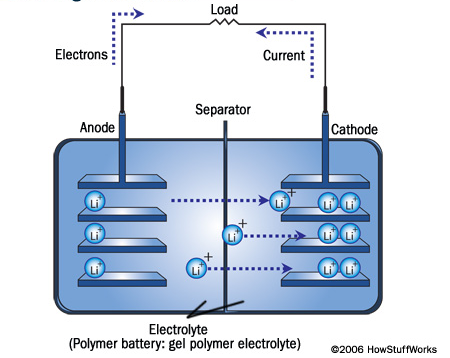
\includegraphics[width=0.6\columnwidth]{images/Schematischer_Aufbau_Li_Ionen.png}
	\caption{Schematischer Aufbau einer Lithium-Ionen-Batterie \cite{howstuffworks}}
	\label{schema_li_ionen}
\end{figure}
Die Elektrochemie einer Batteriezelle basiert auf einem Potential zwischen zwei räumlich getrennten Materialien. Durch den Anschluss eines externen Stromkreises kann dieses Potential entweder unter Abgabe von Energie abgebaut oder unter Zugabe von Energie vergrößert werden \cite{mortimer}. Dabei wird die Elektrode mit dem niedrigeren Halbzellenpotential als Anode, die Elektrode mit dem höheren Halbzellenpotential als Kathode bezeichnet. Zwischen den beiden Elektroden existiert ein Elektrolyt. Dieser ermöglicht den Ladungsaustausch beider Elektroden über den Transfer von Ionen. Um einen Kurzschluss, also einen direkten Ladungsaustausch zwischen beiden Elektroden, zu vermeiden, kann es außerdem nötig sein, einen Separator zwischen beiden Elektroden einzusetzen. Die beiden Elektroden sind jeweils auf einem Stromkollektor aufgebracht, welcher die Kontaktierung der Elektrode nach außen hin ermöglicht \cite{korthauer2013}.
\\\\
Es existieren zwei grundsätzliche Mechanismen zur Ladungsübertragung und Speicherung:
\\\\ %Besser: Unterschiedung reiner Einbau vs. Neubildung von Struktur ???
\textbf{i) Interkalation}
\\\\
Bei der Interkalation handelt es sich um den reinen Einbau eines Atoms oder Ions in ein Wirtsgitter hinein, ohne das Stattfinden einer Reaktion. Beispiel wäre hier der Einbau von Lithiumkationen in eine Graphitstruktur. Bei einer Interkalation kommt es nicht zum Übertrag von Elektronen.
\\\\
\textbf{ii) Redoxreaktion}
\\\\
Während der Redoxreaktion kommt es zu einem Austausch von Elektronen zwischen verschiedenen Edukten. Der reduzierte, also elektronenaufnehmende, und der oxidierte, also elektronenabgebende, Part können dabei räumlich getrennt in den jeweiligen Elektroden vorliegen.
\\\\
Im Falle einer \ce{LiCoO2}-Batterie mit graphitischer Anode wären die bei der Entladung ablaufenden Reaktionen \cite{minakshi2008book}:
\\\\
An der Anode:\\ %Das mit der Interkalation dringend nochmal recherchieren!!!
\begin{equation}
	\ce{Li1C6 -> C6 + Li+ + e-}
\end{equation}
An der Kathode:\\ %Kein vollständiger Ausbau! Korrigieren!
\begin{equation}
	\ce{Li+ + e- + 2Li_{0,5}CoO2 -> 2LiCoO2}
\end{equation}
\subsubsection{Bestimmung der Potentialdifferenz}
Das Potential zwischen zwei Materialien kann als Differenz ihrer jeweiligen Nernstschen Halbzellenpotentiale bestimmt werden. Die Nernst-Gleichung definiert \cite{atkins2006physical}:
\begin{equation}
E = E_0 + \frac{RT}{z_eF}\; ln \frac{a_{Ox}}{a_{Red}}
\end{equation}
mit:
\begin{description}\itemsep0pt
\item[E] Elektrodenpotential
\item[E$_0$] Standardelektrodenpotential
\item[R] Gaskonstante
\item[T] absolute Temperatur
\item[z$_e$] Anzahl der übertragenen Elektronen
\item[F] Faraday-Konstante
\item[a] Aktivität des betreffenden Redox-Partners
\end{description}
Das Verhältnis der Aktivitäten kann dabei als Konzentrationsverhältnis der beiden Phasen dargestellt werden. Einsetzen der Naturkonstanten ergibt als vereinfachte Formel unter der Bedingung eines Betriebes bei Raumtemperatur:
\begin{equation}
E = E_0 + \frac{0,059 V}{z_e} \; log \frac{c_{Ox}}{c_{Red}}
\end{equation}
Über die molare freie Reaktionsenthalpie $\Delta G_m$ kann die Potentialdifferenz als theoretische Zellspannung ebenfalls dargestellt werden \cite{mortimer}:
\begin{equation}
\Delta U_{theo} = -\frac{\Delta G_m}{z_eF}
\end{equation}
Eine einfache Darstellung ist die Angabe des Potentials jedes Stoffes zu reinem Lithiummetall. Die Leerlaufspannung einer Vollzelle ergibt sich dann aus der Differenz zwischen Kathoden- und Anodenspannung gegenüber Lithiummetall:
\begin{equation}
U_{Zelle} = U_{Kathode} - U_{Anode}
\end{equation}
So gilt für eine \ce{LiCoO2}-Zelle mit graphitischer Anode ein mittleres Elektrodenpotential der Kathode gegen Lithium von 3,9V, der Anode von ungefähr 0,1V \cite{bub_skript}. Die Zelle erreicht daher eine theoretische Zellspannung von 3,8V.
\subsection{Elektrodenmaterialien}
Materialien müssen verschiedene chemische und physikalische Eigenschaften erfüllen, um für den Einsatz in Elektroden geeignet zu sein. Die eingesetzten Stoffe sollten ungiftig sein und in ausreichender Menge günstig zu beschaffen sein. Sie sollten eine ausreichend hohe Potentialdifferenz zwischen den Elektroden besitzen, um eine hohe Zellspannung gewährleisten zu können. Das Material sollte eine möglichs hohe Energie- und Leistungssdichte ermöglichen, um auch für den mobilen Einsatz interessant zu sein. Es muss sowohl eine gute Lithium- als auch Elektronenleitfähigkeit gewährleistet sein. Die Ein- und Auslagerung von Lithium sollte nicht zu einer zu hohen Veränderung des Volumens führen, da diese unter Umstände Grenzflächen zerstört und hohe Anforderungen an die Bauweise der Zellen stellt. Auch nach einer hohen Anzahl an Zyklierungen sollte das Material noch eine ausreichende Kapazität besitzen. Ein Versagen der Zelle sollte möglichst nicht zu einer starken Hitzeentwicklung und Explosion der Zelle führen.
\\\\
Die Materialien für Elektroden können grundsätzlich nach ihrem Diffusionsverhalten klassifiziert werden \cite{graf2013kathodenmaterialien}:
\begin{description}
\item[Olivinstruktur] Die Olivinstruktur ist eine eindimensionale Tunnelstruktur, an der entlang die Diffusion stattfindet. Dies sind in der Regel Phosphate wie das \ce{LiFePO4}.
\item[Lagenstruktur] Materialien, die zweidimensionale Diffusion zwischen Schichten ermöglichen, besitzen eine Lagenstruktur.
\item[Spinellstruktur] In der Spinellstruktur ist eine Diffusion in alle drei Richtungen des Raums möglich.
\end{description}
Eine Übersicht über die verschiedenen Kanalstrukturen und deren mögliche Elektrodenmaterialien findet sich in Abbildung \ref{strukturen_elektroden}.
\begin{figure}
	\centering
	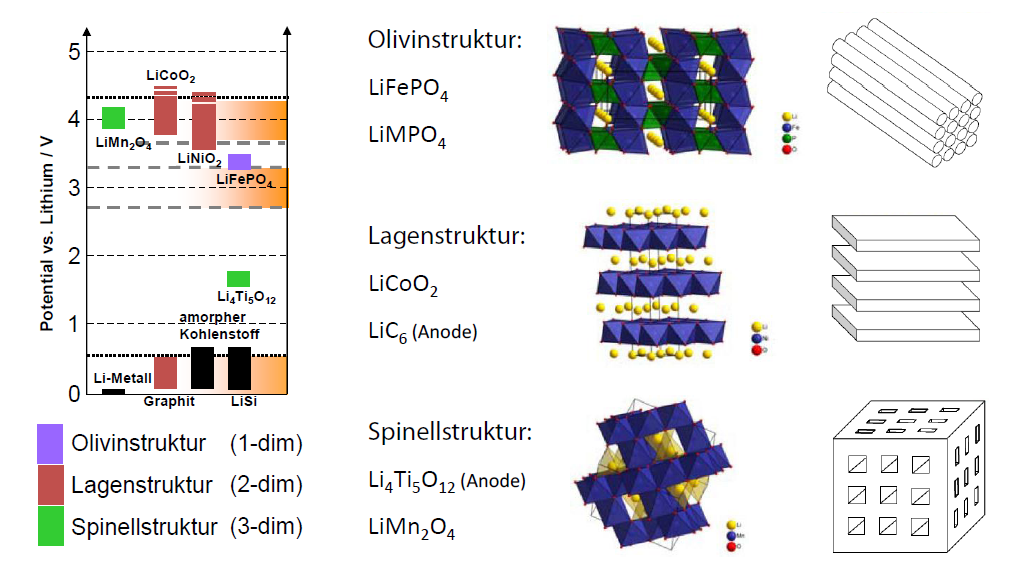
\includegraphics[width=1.0\columnwidth]{images/strukturen_elektroden.png}
	\caption{Potentiallagen verschiedener Elektrodenmaterialien (links) und die ihrere Diffusion zugrundeliegenden Kanalstrukturen (rechts) \cite{bub_skript}}
	\label{strukturen_elektroden}
\end{figure}
\subsubsection{Typische Anodenmaterialien}
% Was zur SEI schreiben? Quelle Skript BuB?
Für die meisten Zellen in dieser Arbeit kamen metallische Lithiumanoden zum Einsatz. Kommerziell ist Graphit momentan das Standardanodenmaterial von Lithium-Ionen-Batterien. Ein keramisches Material, das sich als Anode eignet, ist das Lithiumtitanat.
\begin{description}
\item[Lithium-Metall] Rein metallisches Lithium besitzt eine sehr hohe theoretische Kapazität von 3860mAh/g \cite{jossen_2006}. Da jedoch die Anode im Betrieb nicht aufgebraucht werden darf, muss es im Überschuss bereit gestellt werden. Problematisch ist, dass es durch das fehlende Wirtsgitter dazu neigt während der Zyklierung Dendriten auszubilden, die schlussendlich zu einem Kurzschluss und Ausfall der Zelle führen \cite{aurbach2002short}. 
\item[Graphit (\ce{C6})] Graphit besitzt eine Lagenstruktur zwischen der er Lithium einspeichern kann. Es kann jeweils ein Lithiumatom pro sechs Kohlenstoffatomen eingelagert werden. Er erreicht damit eine theoretische Kapazität von 372 mAh/g \cite{delasCasas201274}. Das Potential gegen rein metallisches Lithium ist sehr klein (ca. 0,1V), was hohe Zellspannungen ermöglicht. Die Einlagerung erfolgt über drei unterschiedliche Stufen und führt zu einer Volumenzunahme von maximal 9\% \cite{bub_skript}.
\item[Lithiumtitanat (\ce{Li4Ti5O12}, LTO)] Teilweise auch Lithiumtitanspinell. Lithiumtitanat besitzt eine Spinellstruktur. Die theoretische Kapazität liegt bei 233mAh/g, in der Praxis werden meistens Kapazitäten von 150mAh/g - 175mAh/g erreicht. Das Material vollführt nahezu keine Volumenänderung bei Ein- und Ausbau von Lithium \cite{huang2007effects}. Jedoch ist seine Potentiallage mit 1,55V gegenüber metallischem Lithium sehr hoch, was zu kleineren Zellspannungen führt \cite{hong2010effect}.
\end{description}
\subsubsection{Typische Kathodenmaterialien}
Sony etablierte in den 90er Jahren das Lithiumcobaltdioxid als Standardkathodenmaterial. Bis heute zählt es zu den meistgenutzen Materialien in Lithium-Ionen-Batterien. Aktuelle Forschungen finden aber auch mit dem Lithiummanganspinell und Schwefel statt.
\begin{description}
\item[Lithiumcobaltdioxid (\ce{LiCoO2})] Die praktische Kapazität von Lithiumcobaltoxid liegt bei 150mAh/g. Dies liegt an der Tatsache, dass nur etwa 60\% der Lithiumatome aus dem Gitter ausgebaut werden dürfen, da es sonst durch den Zusammenbruch der Struktur zur Bildung von Sauerstoff kommt \cite{jossen_2006}. Beim Laden muss die Spannung deshalb unter 4,2V gehalten werden. Die Diffusion läuft zweidimensional zwischen zwei Schichten ab. Das mittlere Elektrodenpotential von Lithiumcobaltoxid liegt bei hohen 3,9V.
\item[Lithiummanganspinell (\ce{LiMn2O4}, LMO)] Lithiummanganspinell ist ein Hochvolkathodenmaterial, sein mittleres Elektrodenpotential liegt bei 4,0V. Die praktische Kapazität des Stoffes liegt bei etwa 120mAh/g bei der Verwendung von Flüssigelektrolyten, welche die Ladespannung  begrenzen \cite{Wang2008developments}. Der Spinell selbst ist auch noch bei höheren Potentialen stabil. Bei tiefen Ladezuständen kann es zu einer Manganauslösung und unerwünschten Gitterumwandlungen kommen, der Jahn-Teller-Verzerrung. Um diese zu verhindern, können Teile des Mangans durch andere Übergangsmetalle substituiert werden \cite{bhaskar20143d}.
\item[Schwefel] Reiner Schwefel besitzt normalerweise einen zyklischen Achterring. Beim Einsatz als Kathodenmaterial wird dieser Ring beim Entladen langsam reduziert und es entstehen verschiedene Polysulfide:
\begin{equation}
\begin{split}
\ce{S8 -> Li2S8 -> Li2S6 -> Li2S5 -> }\\
\ce{ Li2S4 -> Li2S3 -> Li2S2 -> Li2S}
\end{split}
\end{equation}
Diese existieren in unterschiedlichen Konzentrationen auch nebeneinander, der Schwefelanteil am Gemisch nimmt aber während dem Entladevorgang ab. Dieser Vorgang findet reversibel beim Laden der Zelle statt \cite{zhang2013liquid}. Die theoretische Kapazität einer Lithium-Schwefel-Zelle liegt bei 1672mAh/g, praktisch kann aber momentan bei höheren Lade/Entladeraten jedoch nur ein um den Faktor 5-10 niedrigerer Wert erreicht werden. Das größte Problem des Materials sind ungewollte Reaktionen der Polysulfide und ein damit einhergehender Verlust an Aktivmaterial und eine schleichende Vergiftung des Elektrolyten. Beides schädigt der Materialausnutzung und sorgt für eine schlechte Zyklenstabilität \cite{manthiram2012challenges}.
\end{description}
Alle Kathodenmaterialien und auch das Anodenmaterial LTO besitzen eine zu schwache Leitfähigkeit für Elektronen. Daher wird ihnen Kohlenstoff beigemischt, um Elektronen in die Elektrode zu transportieren. Die Materialien werden dabei mit Bindern versetzt, um für eine gute Suspension zwischen den Materialien und innerhalb der Elektrodenfolie zu sorgen. Die optimale Auswahl an Kohlenstoffmodifikation (Ruß, Graphit, Kohlenstoffnanoröhrchen, Graphen) und deren Prozessierung ist dabei eine aktuelle Forschungsaktivität (\cite{kucinskis2013graphene}, \cite{guo2015microporous}). Es wird eine möglichst geringe Beimischung dieser Zusatzstoffe angestrebt, um die Masse an Aktivmaterial in der Zelle zu optimieren.
\subsection{Elektrolyte}
\begin{figure}
	\centering
	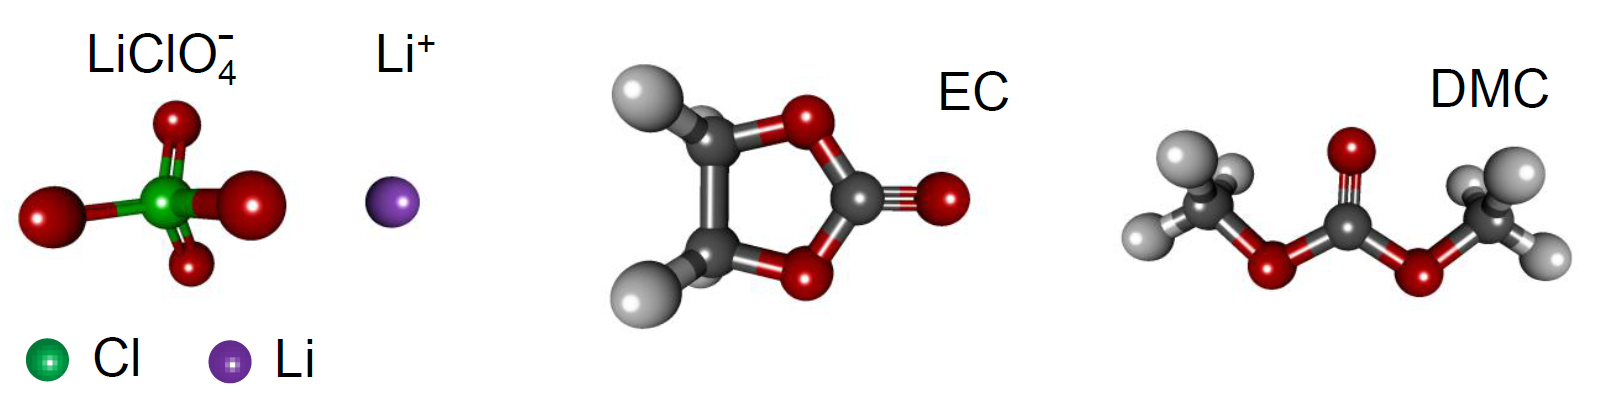
\includegraphics[width=1.0\columnwidth]{images/fluessigelektrolyt.png}
	\caption{Chemische Strukturen der Bestandteile eines Flüssigelektrolyten \cite{bub_skript}}
	\label{fluessigelektrolyt}
\end{figure}
Elektrolyte sollen möglichst wenig elektronenleitend sein, um eine schleichende Selbstentladung der Batterie zu verhindern. Gleichzeitig muss aber eine gute Ionenleitfähigkeit gewährleistet werden, um eine hohe Leistung der Zelle zu ermöglichen. Weiterhin müssen die Grenzflächen zwischen Elektrode und Elektrolyt eine ausreichende Güte besitzen, damit die Ionen zwischen beiden Zellbestandteilen wandern können.
\\\\
Als Elektrolyt kommen kommerziell fast ausschließlich Flüssigelektrolyte zum Einsatz. Diese bestehen aus einem organischen Lösungsmittel wie beispielsweise einer Ethylencarbonat-Dimethylcarbonat-Mischung (EC-DMC). Hier sorgt das stark polare Ethylencarbonat für die Löslichkeit, während man mit dem Dimethylcarbonat-Anteil die Viskosität der Lösung einstellen kann. In diese Mischung löst man dann ungesättigte Lithium-Leitsalze wie \ce{LiPF6}, \ce{LiAsF6} oder \ce{LiClO4}. Eine Abbildung der chemischen Strukturen der Bestandteile eines Flüssigelektrolyten auf EC/DMC-Basis mit \ce{LiClO4} als Leitsalz ist in Abbildung \ref{fluessigelektrolyt} dargestellt.
\\\\
Problem dieser Lösungen sind ihre schlechte Beständigkeit gegenüber Wasser. Bei \ce{LiPF6} sorgen beispielsweise schon kleinste Verunreinigungen des Elektrolyts zur Bildung von hochätzender Flusssäure, die den Elektrolyt vergiftet und zu einem Ausfall der Zelle führt \cite{xu2004nonaqueous}. Dies ist bei der Herstellung von Lithium-Ionen-Batterien ein großes Problem, da es eine aufwendige und teure Trocknung der Luft bei der Herstellung der Zellen erfordert.
\\\\
Ein weiteres Problem von Flüssigelektrolyten ist ihr begrenztes Temperaturfenster. Bei zu hohen Temperaturen verdampft der Elektrolyt und zerstört so die Zelle, bei zu niedrigeren Temperaturen bildet sich zumeist ein Polymergel, welches nicht mehr in der Lage ist die Ionen zu leiten \cite{blomgren2003liquid}.
\subsection{Potentialuntersuchung mit zyklischer Voltametrie}
Bei der zyklischen Voltametrie wird zuerst ein ansteigendes und anschließend ein abfallendes Potential an eine Batterie angelegt. Gemessen wird die sich bei den unterschiedlichen Potentialen ergebende Stromstärke. Diese ist ein Maß dafür, ob eine elektrochemische Reaktion innerhalb der Batterie stattfindet. Diese stellt sich als ein Peak innerhalb des Diagramms der zyklischen Voltametrie dar. Es kann dabei zwischen oxidierenden und reduzierenden Reaktionen unterschieden werden, je nachdem ob ein Peak im ansteigenden oder im abfallenden Potentialbereich auftritt \cite{Hamann2005}.
\\\\
Die zyklische Voltametrie ist insbesondere dazu geeignet, zu verstehen bei welchen Spannungen Reaktionen ablaufen und ob diese reversibel sind. Sie ermöglicht damit das exakte Einstellen von Arbeitsspannungen zum Laden und Entladen von Batteriezellen, die nicht über- oder unterschritten werden sollten \cite{Linden2011}.
\subsection{Grenzschichtcharakterisierung durch Impedanzspektroskopie}
Die Impedanzspektroskopie eignet sich, um Widerstände und Kapazitäten in einem Gesamtsystem genauer zu untersuchen und dadurch Aussagen über die Leitung und die Grenzschichten innerhalb des Systems treffen zu können.
\\\\
Die Grundlage der Impedanzspektroskopie ist, dass kapazitive und induktive Bauelemente einen sich über den Zeitverlauf ändernden Widerstand besitzen. Werden diese nun in einem Wechselstrom betrieben, so entsteht ein frequenzabhängiger Widerstand, die Impedanz. Eine Impedanz ist aufgebaut aus einem realen, frequenz\-unabhängigen und einem komplexen, frequenz\-abhängigen Teil.
\begin{figure}
	\centering
	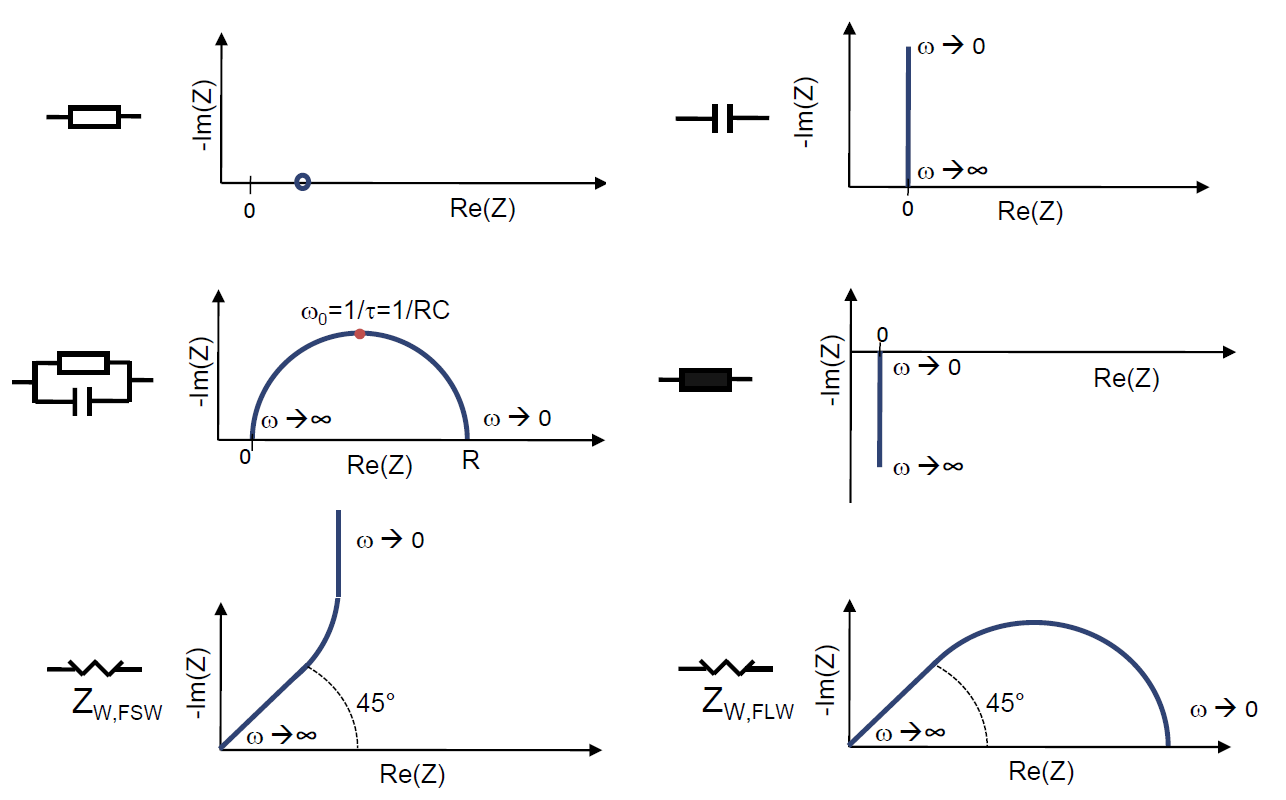
\includegraphics[width=0.9\columnwidth]{images/is_bauteile.png}
	\caption{Ideale Darstellung verschiedener elektrotechnischer Bauteile bei der Impedanzspektroskopie im Nyquist-Plot \cite{bub_skript}}
	\label{bauteile_is}
\end{figure}
\begin{figure}[b]
	\centering
	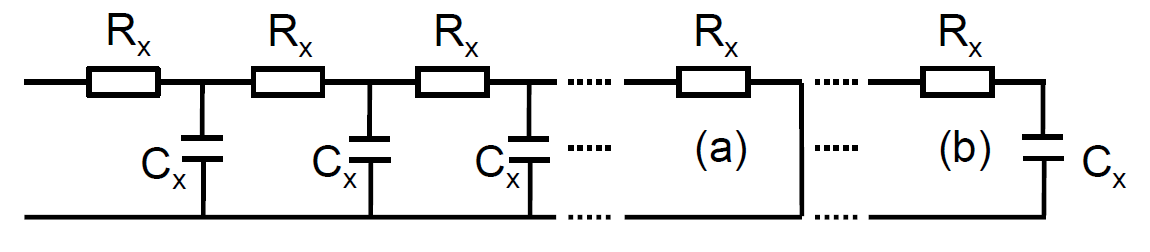
\includegraphics[width=0.8\columnwidth]{images/warburg_element.png}
	\caption{Kettenleitermodell eines Finite-Length (a) und Finite-Space (b) Warburg-Elements \cite{bub_skript}}
	\label{warburg_element}
\end{figure}
\subsubsection{Elektrochemisches Ersatzschaltbild}
Elektrotechnische Bauelemente besitzen nun unterschiedliche, charakteristische Impedanzen. Eine Verschaltung unterschiedlicher Elemente resultiert in einem Impedanzspektrum. Dargestellt werden können diese in einem Nyquist-Plot, der den Realteil gegen den Imaginärteil aufträgt \cite{Hamann2005}. Eine Übersicht über alle Bauteile und ihre korrespondierenden Nyquist-Plots findet sich in Abbildung \ref{bauteile_is}.
% Dazu schreiben, wo in einer Batterie das auftritt
\begin{description}
\item[Widerstand] Der Widerstand besitzt keinen komplexen, sondern lediglich einen realen Anteil. Dies entspricht einem Punkt auf der Realachse des Nyquist-Plots.
\item[Kondensator] Ein idealer Kondensator besitzt keinen realen Widerstand. Sein Imaginärteil konvergiert bei hohen Frequenzen gegen Null, bei niedrigen Frequenzen divergiert er ins Negative.
\item[Spule] Eine Spule besitzt ebenfalls keinen realen, sondern nur einen imaginären Widerstand. Dieser konvergiert für niedrige Frequenzen gegen Null, bei hohen Frequenzen divergiert er ins Positive
\item[RC-Glied] Grenzflächen, beispielsweise zwischen Elektrode und Elektrolyt in einer Batterie, bilden meistens sogenannte Helmholtz-Doppelschichten aus. Sie besitzen sowohl ein kapazitives Element als auch einen Durchtrittswiderstand. Dies kann als RC-Glied, also einer Parallelschaltung von Widerstand und Kondensator, dargestellt werden. Im Nyquist-Plot ergibt sich ein Halbkreis mit Radius 1/RC.
\item[Warburg-Element] Um Diffusionprozesse darzustellen, können Warburg-Elemente verwendet werden. Diese leiten sich aus den Fickschen Gesetzen her. Sie bestehen aus einem Kettenleitermodell aus Widerständen und Kondensatoren, wobei zwischen Finite-Length und Finite-Space Warburg-Elementen unterschieden werden muss (siehe Abbildung \ref{warburg_element}).
\end{description}
Das Impedanzspektrum einer Batterie kann mit Hilfe eines elektrochemischen Ersatzschaltbildes analysiert werden. Dabei versucht man für ein experimentell erhaltenes Impedanzspektrum ein plausibles Ersatzschaltbild zu finden, dessen Impedanzspektrum vom experimentell bestimmte Spektrum möglichst wenig abweicht. Ein Beispiel hierfür lässt sich in Abbildung \ref{schema_is} finden.
\\\\
Aus dem so modellierten Ersatzschaltbild lassen sich quantitative Aussagen über die einzelnen Widerstände und Grenzschichten innerhalb einer Batteriezelle treffen. Das Impedanzspektrum ist bei einer Batterie jedoch auch immer von Faktoren wie dem Ladezustand, der Temperatur oder der Anzahl an bereits erfolgter Zyklen abhängig \cite{Linden2011}.
\begin{figure}
	\centering
	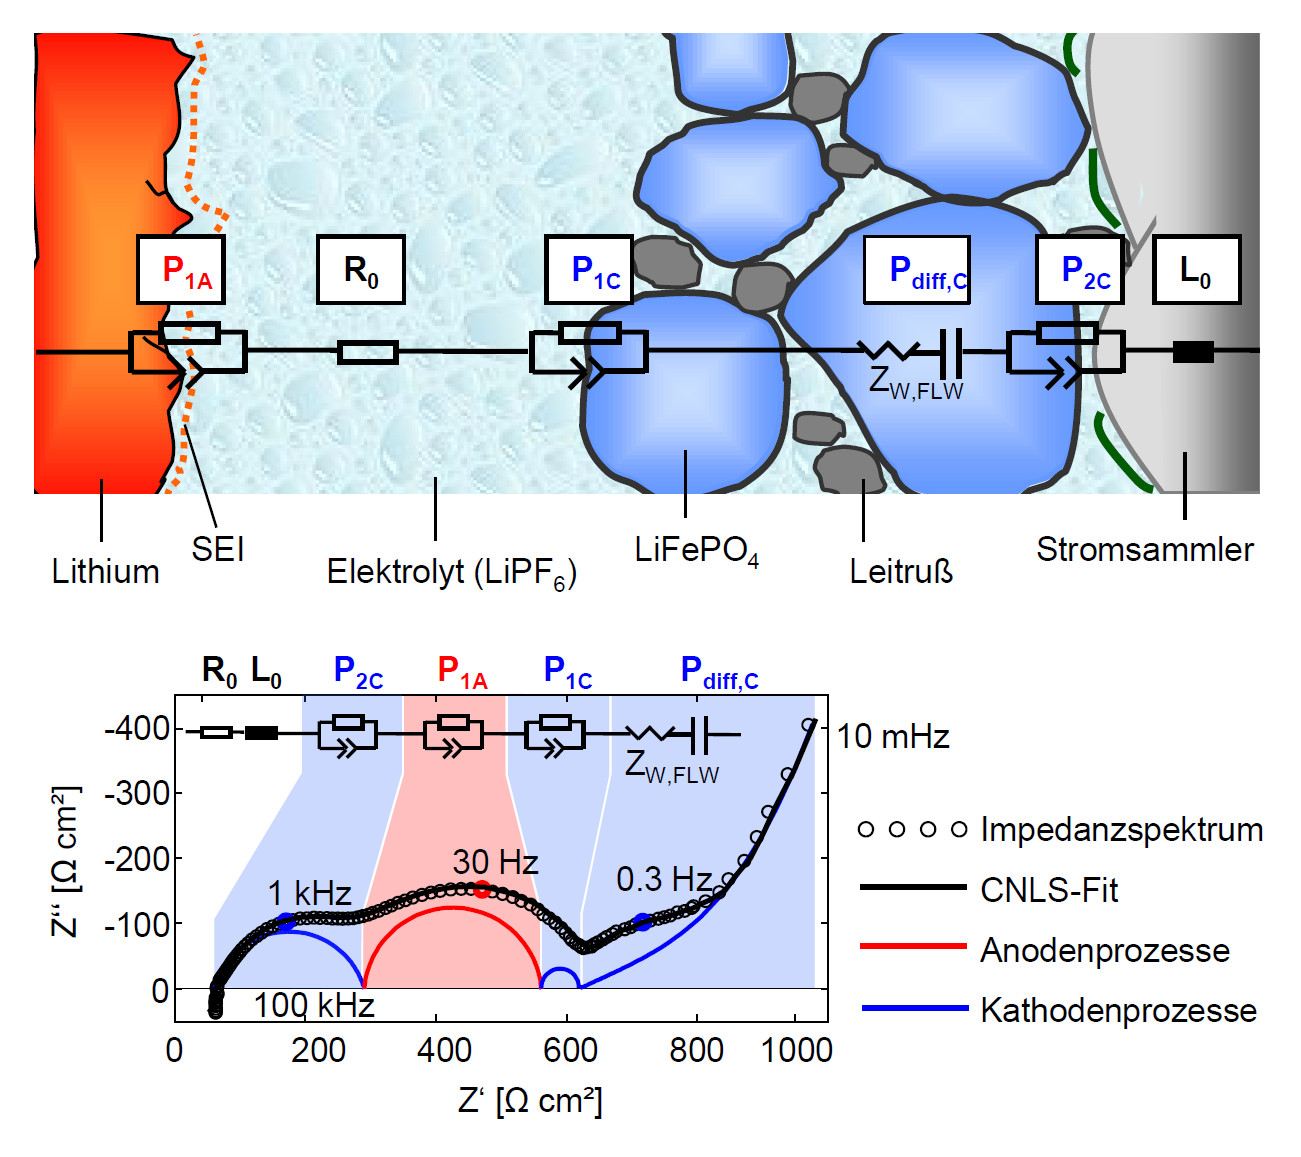
\includegraphics[width=0.8\columnwidth]{images/Schema_IS.jpg}
	\caption{Elektrochemisches Ersatzschaltbild und resultierendes Impedanzspektrum in Nyquist-Darstellung einer Li-\ce{LiFePO4}-Zelle \cite{bub_skript}}
	\label{schema_is}
\end{figure}
\section{Keramiken für den Einsatz als Festkörperelektrolyt}
\label{grundlagen_keramik}
Keramiken sind anorganische, nicht-metallische und polykristalline Werkstoffe. Es existieren verschiedene Keramiken, welche in der Lage sind Lithium-Ionen zu leiten. Grundsätzlich lassen sich dabei basierend auf der Struktur der Werkstoffe verschiedene Klassen von lithiumleitenden Keramiken identifizieren. Dazu zählen die Perowskite, Granate, keramische Gläser, amorphe Keramiken sowie die Na-Super-Ionic-Conductor (NASICON) Keramiken \cite{tatsumisago2013recent}. In dieser Arbeit werden Keramiken auf Perowskit- und NASICON-Basis untersucht.
\subsection{Perowskite}
\begin{figure}
	\centering
	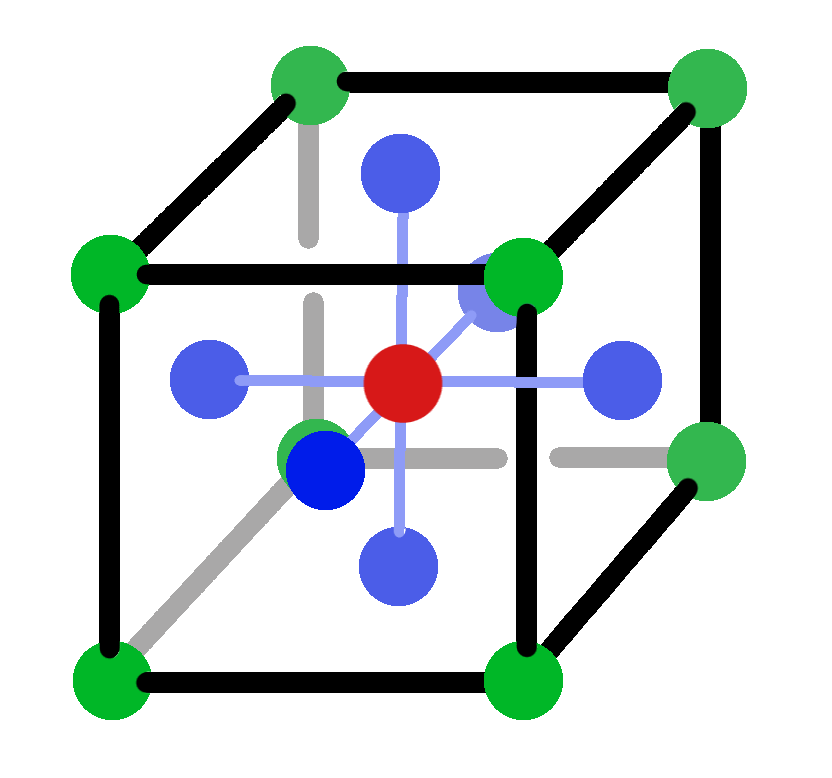
\includegraphics[width=0.45\columnwidth]{images/Perowskit-Struktur.png}
	\caption{\ce{ABO3}-Struktur eines Perowskits (blau: A, rot: B, grün: O)}
	\label{struktur-perowskit}
\end{figure}
Perowskite folgen der Struktur \ce{ABO_3}. Sie sind kubisch-flächenzentriert aufgebaut mit dem B-Element in der Mitte, den A-Elementen an den Ecken und dem Sauerstoff auf den Flächen. Der Sauerstoff ist zweifach negativ geladen. Damit ergibt sich für die Kombination aus A und B eine notwendige sechsfach positive Gesamtladung \cite{ishihara2009perovskite}.
\\\\
Ein vielversprechendes Material für den Einsatz als Festkörperelektrolyt ist hier das Lithiumlanthantitanat (\ce{LiLaTiO3}, LLTO). Das einfach positive Lithium und das dreifach positive Lanthan besetzen dabei die A-Plätze, das vierfach positive Titan den B-Platz. Mögliche Strukturen des LLTO können daher über die Formel \ce{Li_{3x}La_{2/3-x}TiO3} mit $x \in (0, 1/6)$ beschrieben werden. Der Anteil an Leerstellen in der Struktur steigt mit größerem x an \cite{chen2015lithium}.
\\\\
Durch die Leerstellen auf den A-Plätzen und durch Diffusion können Lithiumionen durch das Material wandern. Dabei bilden jeweils vier Sauerstoffionen eine Flaschenhalsformation \cite{cao2014recent}. Durch eine unterschiedliche Neigung der TiO6-Oktaeder ist der Diffusionswiderstand und die Aktivierungsenergie allerdings im Material inhomogen verteilt. Da sich im Material außerdem entlang der c-Achse lanthanreiche und lanthanarme Schichten bilden, ist die Leerstellenbewegung zwischen diesen Ebenen teilweise gehemmt \cite{jay2015genetics}.
\\\\
Für Lithiumlanthantitanat konnte eine Bulk-Leitfähigkeit von bis zu 1x$10^{-3}$ S/cm nachgewiesen werden \cite{stramare2003lithium}, weshalb eine Einsatzmöglichkeit als Festkörperelektrolyt untersucht wird.
\subsection{NASICON-Keramiken}
Das Akronym NASICON steht für \textbf{Na}-\textbf{S}uper-\textbf{I}onic-\textbf{Con}ductor und wurde ursprünglich für spezielle, natriumleitende Keramiken in Natrium-Schwefel-Batterien verwendet \cite{hagman1968crystal}. Heute steht es allerdings für eine ganze Klasse an Keramiken die für den lithiumleitenden Fall mit der allgemeinen Formel \ce{LiM2(PO4)3} beschrieben werden können. Dabei steht der Platzhalter M für ein Element aus der Gruppe Titan (Ti), Zirkon (Zr), Germanium (Ge) oder Hafnium (Hf).
\\\\
Die Struktur der NASICON-Keramiken ist aus \ce{MO6}-Oktaedern und \ce{PO4}-Tetraedern aufgebaut. Dabei verbindet sich ein \ce{PO4}-Tetraeder immer mit vier unterschiedlichen \ce{MO6}-Oktaedern, der wiederum mit sechs unterschiedlichen Tetraedern in Kontakt steht. Zwischen dieser Struktur existieren zwei Zwischengitterplätze, auf dem sich die Lithiumionen aufhalten können \cite{knauth2009inorganic}. Eine Darstellung ist in Abbildung (noch einfügen) ersichtlich.
\\\\
Der Zwischengitterplatz M1 beschreibt dabei einen Raum zwischen zwei \ce{MO6}-Oktaedern entlang der c-Achse. Die M2-Plätze sind hingegen senkrecht zur c-Achse zwischen den Bändern angeordnet. Zwischen diesen Räumen existieren außerdem noch M12 Plätze. Von entscheidender Bedeutung für die Leitfähigkeit des Materials ist nun, welche Größe die Engstelle zwischen den Gitterplätzen einnimmt. Dieser Flaschenhals kann maßgeblich durch die Ionen innerhalb der Gitterstruktur beeinflusst werden \cite{cao2014recent}.
\subsubsection{Lithiumtitanphosphat}
Wählt man als Komponente M Titan, so erhält man Lithiumtitanphosphat (\ce{LiTi2(PO4)3}). Die zueinander passenden Größen von Lithiumionen auf der einen und der Zwischengitterstruktur auf der anderen Seite sorgt für eine sehr gute Leitfähigkeit. Die Lithiumionen besetzen dabei vollständig die M1-Stellen, die M2-Stellen bleiben vollständig unbesetzt \cite{cao2014recent}. 
\\\\
Eine weitere Erhöhung der Bulk-Leitfähigkeit kann durch einen teilweisen Einbau von beweglicheren Aluminiumionen anstelle von Titanionen erzielt werden. Das entstehende Material ist Lithium-Aluminium-Titanphosphat (LATP) und kann durch die allgemeine Struktur \ce{Li_{1+x}Al_{x}Ti_{2-x}(PO4)3} beschrieben werden. Die durch die Substituierung der Titanionen zusätzlich eingebrachten Lithiumionen besetzten dabei M2-Plätze, was zu einer Steigerung der Ionenleitfähigkeit führt \cite{aono1991electrical}. Es konnten Leitfähigkeiten von $7*10^{-4}$ Scm$^{-1}$ nachgewiesen werden \cite{aono1990ionic}. 
\\\\
Die \ce{Ti^{4+}}-Ionen des LATP werden von verschiedenen Anodenmaterialien, wie Lithiummetall oder lithiierten Graphit, zu \ce{Ti^{3+}} reduziert. Diese Instabilität kann zu einem Versagen des Elektrolyts führen. Das LATP muss daher mit einem geeigneten Anodenmaterial kombiniert werden.
\subsubsection{Lithium-Aluminium-Germaniumphosphat}
Um der Reduktion der Titankationen vorzubeugen, können diese mit Germaniumkationen ersetzt werden. Das so entstehende Material ist Lithium-Aluminium-Germaniumphosphat (LAGP). Es kann mit der allgemeinen Struktur \ce{Li_{1+x}Al_xGe_{2-x}(PO4)3} beschrieben werden. LAGP besitzt eine ionische Leitfähigkeit in Höhe von $4*10^{-4}$ Scm$^{-1}$ \cite{fu1997fast}.
% Details zur Herstellung?
\subsection{Pulveranalyse mittels Röntgendiffraktion}
Die Röntgendiffraktion (X-Ray Diffraction, XRD) nutzt den Zustand der charakteristischen Beugung von Röntgenstrahlung an geordneten Strukturen wie Kristallen aus, um daraus Aussagen über diese Struktur treffen zu können. Damit ist es beispielsweise möglich, die Phasenreinheit eines Stoffes zu bestimmen.
\subsubsection{Physikalische Grundlagen der XRD}
Bei der Beugung von Röntgenstrahlen an Kristallgittern entstehen Interferenzen durch die unterschiedlich tiefe Eindringung in das Material bis zum Auftreffen auf ein Teilchen. Dieser Umstand kann mit der Bragg-Gleichung beschrieben werden:
\begin{equation}
n\lambda = 2d \sin{\theta}
\end{equation}
mit
\begin{description}\itemsep0pt
\item[n] Grad des untersuchten Maximums
\item[$\boldsymbol{\lambda}$] Wellenlänge der Röntgenstrahlung
\item[d] Abstand der Netzebenen
\item[$\boldsymbol{\theta}$] Winkel der Strahlung zur Netzebene
\end{description}
Eine schematische Darstellung ist in Abbildung \ref{bragg} gegeben.
% Weitere Beschreibung?
\begin{figure}
	\centering
	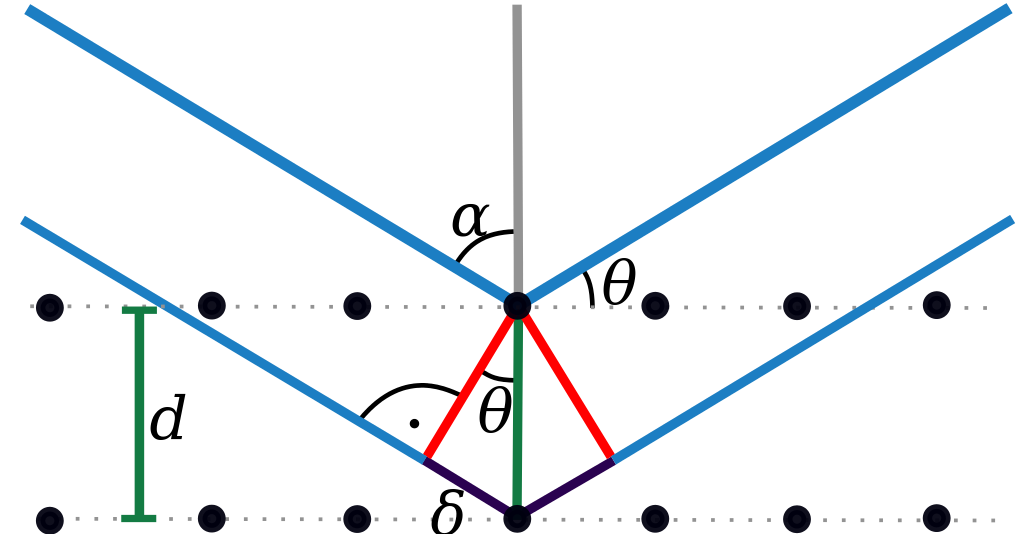
\includegraphics[width=0.6\columnwidth]{images/Bragg.png}
	\caption{Schematische Darstellung der Bragg-Reflexion \cite{wiki_bragg}}
	\label{bragg}
\end{figure}
\subsubsection{Bragg-Brentano-Diffraktometer}
Eine Bragg-Brentano-Anordunung eignet sich besonders für das Anfertigen von Pulverdiffraktogrammen. Eine ebene, flache Probe, z.B. in einen kleinen Tigel gepresstes Pulver, wird im Mittelpunkt eines Drehkreises befestigt. Der Röhrenfokus wird nun im gleichen Abstand zur Probe wie der Detektor angebracht. Beide zeigen im gleichen Winkel auf die Probe. Während der Messung wird dieser Winkel nun kontinuierlich variiert. Dazu kann entweder die Probe mit halber Winkelgeschwindigkeit des Detektors gedreht werden oder Röhre und Detektor bewegen sich mit gleicher Geschwindigkeit aufeinander zu beziehungsweise voneinander weg. Es kann nun für jeden Winkel quantitativ das Maß an Reflexion und Interferenz gemessen werden und daraus ein Diffraktogramm erstellt werden. Mittels Rietveld-Methode oder Vergleich mit einer Datenbank ist anschließend eine Analyse des Diffraktogramms möglich \cite{krischner1994}.
% Evtl. noch eine Grafik?
%\section{Analysemethoden}
%Zur Strukturaufklärung werden die Materialien mit drei unterschiedlichen Analysemethoden untersucht. Die Röntgendiffraktion misst Reflexionen und Interferenzen an Kristallgittern und ermöglicht daher eine Charakterisierung der untersuchten Stoffe über ihre kristalline Struktur. Bei der Impedanzspektroskopie wird der frequenzabhängige, komplexe Widerstand eines Materials untersucht, um dessen Leitfähigkeit genauer analysieren zu können. Die Kernspinspektroskopie ermöglicht die genaue Untersuchung der atomaren Umgebung eines speziellen Elements innerhalb einer Struktur durch gezieltes Ausrichten und Variieren der Kernspins.
\section{Kernspinresonanzspektroskopie}
%Motivation NMR
Die Grundlage der Kernspinresonanzspektroskopie (nuclear magnetic resonance spectroscopy, NMR-Spektroskopie) wurde zum Jahreswechsel 1945/1946 von zwei amerikanischen Forschungsgruppen unabhängig voneinander entwickelt. Felix Bloch und Edward M. Purcell wurden dafür 1952 mit dem Nobelpreis in Physik ausgezeichnet.
\subsection{Physikalische Grundlagen der NMR-Spektroskopie}
Die NMR-Spektroskopie nutzt die magnetischen Eigenschaften von Atomkernen und ihren Umgebungen aus, um Aussagen über Zusammensetzungen und Bindungen von Stoffen treffen zu können.
\\\\
Elektronen, Neutronen und Protonen besitzen eine Eigenrotation, den Spin s. Der Spin eines Atomkerns setzt sich aus den Spins der einzelnen Protonen und Neutronen innerhalb des Kerns zusammen. Spins sind gequantelt und können daher nur gewisse diskrete Zustände annehmen. Dies gilt auch für den resultierenden Gesamtspin des Atomkerns. Die möglichen Zustände des Kernspins eines spezifischen Isotops können beschrieben werden über seine Spinquantenzahl I. Es existieren folgende magnetische Spinquantenzahlen m, welche die möglichen Orientierungen des Spins beschreiben \cite{Gerthsen2015}:
\begin{equation}
m_I = I, I-1, I-2, ..., -I
\end{equation}
Die Gesamtzahl an möglichen Zuständen entspricht daher der Summe von 2I+1. Das Li$^7$ besitzt die Spinquantenzahl I=$\frac{3}{2}$ \cite{Fitzgerald1999}. Es gilt daher:
\begin{equation}
m_{I=\frac{3}{2}} = \frac{3}{2}, \frac{1}{2}, -\frac{1}{2}, -\frac{3}{2}
\end{equation}
Sind in einem Atomkern die Anzahl an Protonen und Neutronen beide gerade, so gilt für die Spinquantenzahl I=0. Ein solcher Nukleus besitzt keinen Kernspin und kann daher nicht mittels NMR-Spektroskopie untersucht werden.
\\\\
Ein Atomkern besitzt eine Ladung. Wenn diese durch einen Kernspin bewegt wird, so besitzt der Nukleus ein magnetisches Moment $\mu$ in Abhängigkeit zum Zustand des Spins. Der Zusammenhang zwischen einem Drehmoment P und dem magnetischen Moment kann allgemein über das gyromagnetische Verhältnis $\gamma$ beschrieben werden \cite{Guenther2013}: 
\begin{equation}
\mu = \gamma P
\end{equation}
Das Drehmoment des Kerns in Richtung z eines frei gewählten kartesischen Koordinatensystems entspricht dabei seiner magnetischen Spinquantenzahl multipliziert mit dem reduzierten Planckschen Wirkungsquantum:
\begin{equation}
P_z = m_I \hbar
\label{magnMoment}
\end{equation}
Das magnetische Moment kann also beschrieben werden mit:
\begin{equation}
\mu_z = \gamma m_I \hbar
\end{equation}
Keiner dieser möglichen Spinzustände ist energetisch günstiger als die anderen. Die Zustände liegen daher degeneriert vor. Dies kann allerdings durch das Anlegen eines starken äußeren Magnetfeldes B$_0$ in positiver z-Richtung beeinflusst werden. Es bilden sich verschiedene Energieniveaus für die unterschiedlichen Spinzustände aus. Die Potentialenergie E kann beschrieben werden als:
\begin{equation}
E = -\mu_z B_0
\end{equation}
Mit Einsetzen von Gleichung \ref{magnMoment} ergibt sich daher mit den unterschiedlichen Spinorientierungen $m_I$:
\begin{equation}
E = -m_I \gamma \hbar B_0
\label{energiezustaende}
\end{equation}
Diese Aufspaltung der Energieniveaus ist bekannt als \textit{nuclear Zeeman splitting} \cite{Guenther2013}. 
\\\\
Die Energiedifferenz zwischen den Zuständen ist dabei proportional zur Stärke des angelegten äußeren Magnetfelds. Die Spins richten sich entlang der Achse aus. Die Energiedifferenzen sind dabei für jeden Kern, der einen Spin besitzt, charakteristisch und können mit einer Frequenz in Abhängigkeit zur Stärke des äußeren Magnetfelds beschrieben werden. Mit der \textit{Bohrschen Frequenzbedingung}\cite{Gerthsen2015}:
\begin{equation}
\Delta E = hv
\end{equation}
kann die benötigte Quantenenergie bestimmt werden als: %gilt nur für den Protonenfall?
\begin{equation}
hv_0 = \gamma \hbar B_0
\end{equation}
Dargestellt als Frequenz:
\begin{equation}
\omega_0 = \gamma B_0
\end{equation}
Diese Frequenz wird als \textit{Larmor-Frequenz} bezeichnet und kann auch als Präzession des Kerns beschrieben werden \cite{Guenther2013}. 
\\\\
Wird nun eine Transmitterspule in einem äußeren Magnetfeld $B_0$ mit einer spezifischen Larmor-Frequenz betrieben, so bringt sie exakt die nötige Energiedifferenz ein, um die Spins in einen energiereicheren Zustand zu promovieren. Das dadurch entstehende NMR-Signal kann mit einer Empfängerspule aufgezeichnet werden \cite{Friebolin2011}.
\\\\
Durch chemische Verbindungen entstehen um Atomkerne herum unterschiedlich dichte Elektronenwolken. Diese schirmen den Kern etwas vom äußeren Magnetfeld $B_0$ ab. Es entsteht ein lokales Magnetfeld $B_{lokal}$ um die Kerne herum, welches sich in seiner Stärke vom globalen Magnetfeld unterscheidet. Dadurch variiert die benötigte Anregungsfrequenz je nach der Umgebung eines Kernes leicht. Dieser Effekt findet sich als \textit{chemische Verschiebung} in Gestalt von unterschiedlichen Peaks im NMR-Spektrum wieder. Mit ihr ist es möglich Strukturaussagen über ein untersuchtes Material zu treffen.
\subsection{Aufbau eines NMR-Spektrometers}
\begin{figure}
	\centering
	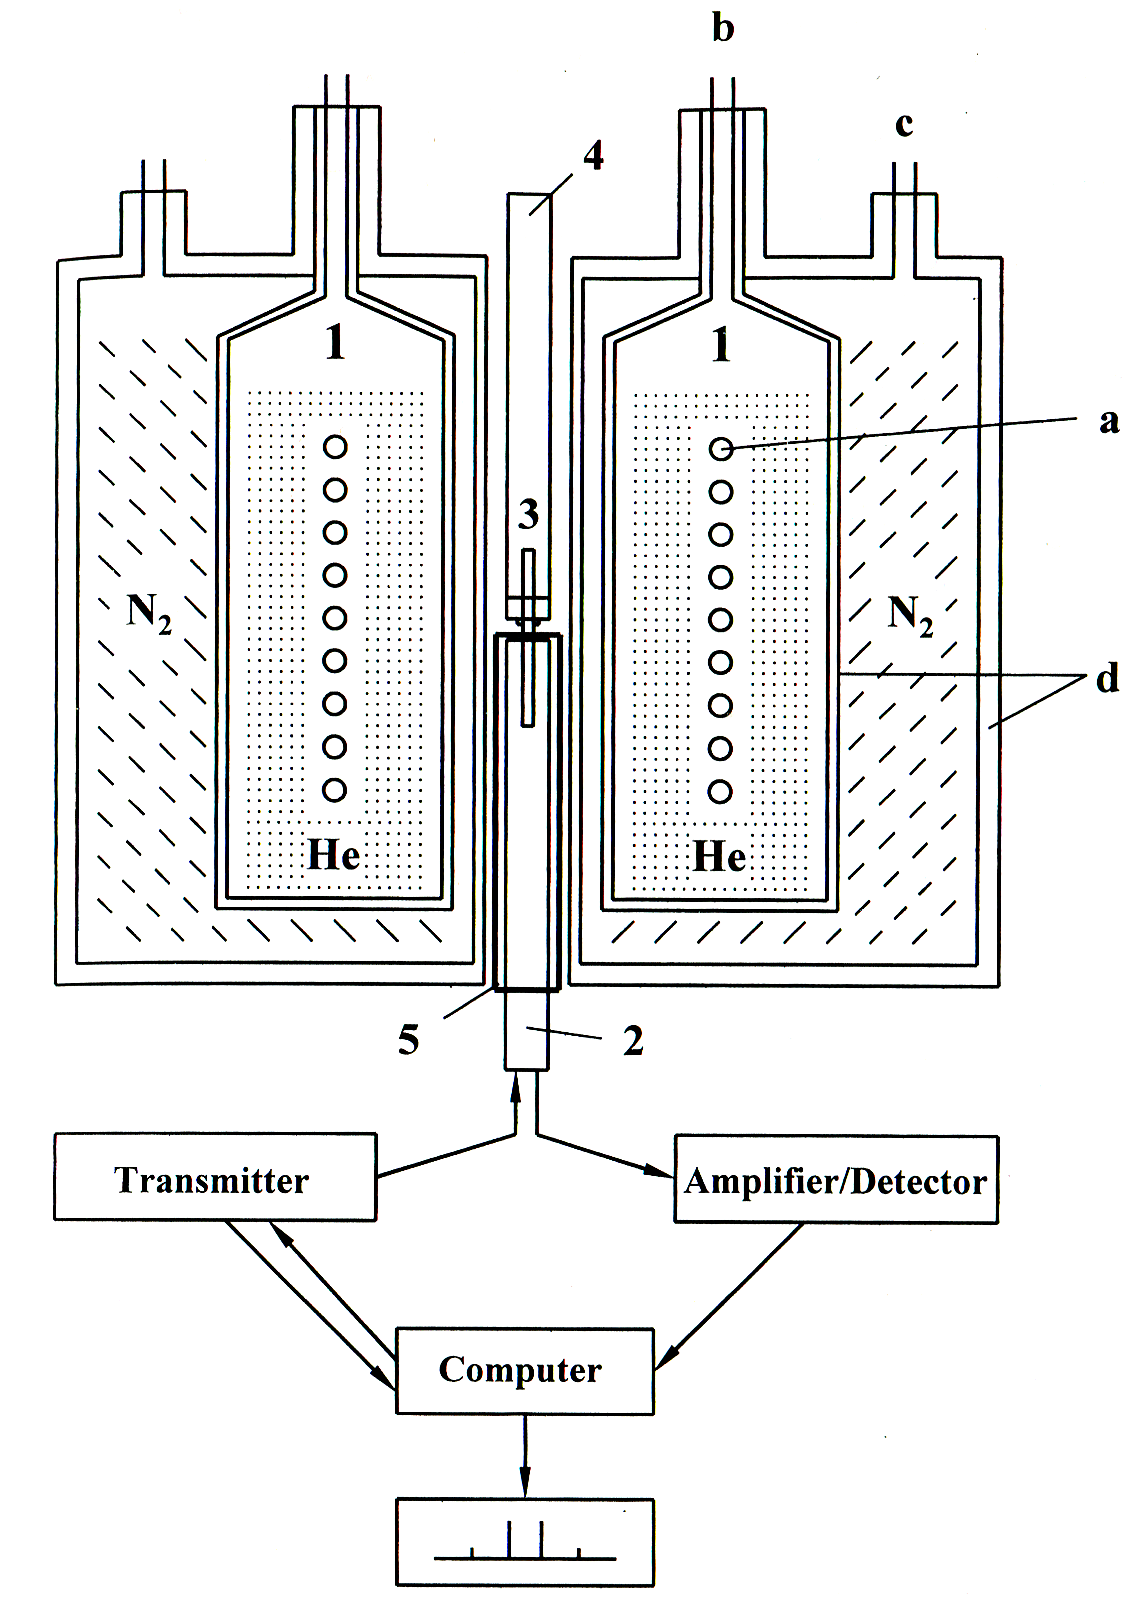
\includegraphics[width=0.9\columnwidth]{images/Aufbau_NMR.png}
	\caption{Schematischer Aufbau eines NMR-Spektrometers. Der Kryomagnetaufbau (1) mit Spule (a), Einfüllstutzen (b, c) und Vakuummänteln (d), Probenkopf (2), Probe (3), Probenwechsler (4) sowie Shim-Einheit (5). }
	\label{aufbau_nmr}
\end{figure}
Aus Gleichung \ref{energiezustaende} wird klar, dass die Größe der Potentialdifferenz zwischen energiereichen und -armen Zuständen mit der Stärke des Magnetfelds $B_0$ ansteigt. Die Kerne liegen dabei in Abhängigkeit zur Energiedifferenz $\Delta E$ boltzmannverteilt im energiereichen und -armen Zustand vor \cite{Guenther2013}:
\begin{equation} %auch hier: Hinterer Teil gilt nur für den Protonenfall
\frac{N_{reich}}{N_{arm}} = \exp{\frac{-\Delta E}{kT}}=\exp{\frac{-\gamma h B_0}{2\pi k T}} \approx 1-\frac{\gamma h B_0}{2 \pi k T}
\end{equation}
Im Falle von H$^1$-NMR liegt die Energiedifferenz bei 0.04 J/mol. Bei Raumtemperatur und einer Magnetfeldstärke von 2,35 T ergibt sich damit eine Übergangswahrscheinlichkeit in den energiereichen Zustand von nur 0,002 \%. Um eine ausreichend gute Sensitivität zu gewährleisten, ist daher ein sehr starkes äußeres Magnetfeld $B_0$ nötig. Dies ist lediglich mit Kryomagneten zu erreichen.
\\\\
Der schematische Aufbau eines NMR-Spektrometers wird in Abbildung \ref{aufbau_nmr} dargestellt. Der Kryomagnetaufbau (1) besteht aus den Spulen (a), welche mit Flüssighelium gekühlt werden. Dieser wird wiederum mit Flüssigstickstoff umspült. Die Kühlflüssigkeiten können über spezielle Einlässe eingefüllt werden (b, c) und befinden sich in Vakuummänteln (d).
\\\\
 Der Probenkopf (2) wird von unten eingeführt und an eine Ansteuerungseinheit angeschlossen, welche die Transmitter- und die Empfängerspule ansteuert sowie das Signal aufzeichnet und ggf. verstärkt. Die Transmitter- und Empfängerspule kann meistens als eine Spule realisiert werden, welche beide Funktionen übernimmt. Sie ist im Probenkopf montiert, genauso wie die Entkoppler- Lock- und Gradientenspulen. Die Probe (3) wird von oben eingeführt, was durch einen Probenwechsler (4) passieren kann. Das äußere Magnetfeld $B_0$ liegt damit in Längsrichtung zur Probe. 
\\\\
Um die Feldhomogenität des eingepulsten Signals zu optimieren kann mit einer Shim-Einheit (5) ein \textit{Shimming} durchgeführt werden. Dieses besteht aus einem \textit{Tuning} und einem \textit{Matching}. Mit dem Tuning wird die durch die eingeführte Probe gedämpfte Empfindlichkeit des Probenkopfes auf die Resonanzfrequenz des zu untersuchenden Kerns eingestellt, um die höchstmögliche Empfindlichkeit zu gewährleisten. Das Matching besteht aus einer Impedanzanpassung, um die maximale Leistung am Probenkopf anliegen zu haben. Der gesamte Aufbau wird von einem Computer gesteuert und überwacht, welcher auch die Signalverarbeitung übernimmt \cite{Friebolin2011}.
\subsection{Betriebsmodi eines NMR-Spektrometers}
% Das hier ist schon arg rudimentär
% Beschreibung der Relaxationsmechanismen?
Es existieren zwei unterschiedliche Verfahren, um ein NMR-Spektrum zu messen. Das ältere von beiden ist das Continuous-Wave-Verfahren (CW). Beim CW-Verfahren wird eine monochromatische Strahlung in die Probe emittiert. Diese wird kontinuirlich variiert und die entsprechende Resonanz gemessen. Problematisch ist dabei vor allem die durch das Abfahren unterschiedlicher Frequenzen sehr lange Messzeit.
\\\\
Heute kommt nahezu ausschließlich das Puls-Fourier-Transform-Verfahren (PFT) zum Einsatz. Hierbei wird ein starker Frequenzpuls über einen Wellenlängenbereich auf die Probe abgegeben. Als Resonanz erhält man dabei einen \textit{Free Induction Decay} (FID), der als eine über den Zeitverlauf geschehende Einpendelbewegung in Larmor-Frequenz der angeregten Kerne beschrieben werden kann. Die sich dabei überlagernden Resonanzen können anschließend über eine Fourier-Transformation zum eigentlichen NMR-Spektrum zurückgerechnet werden \cite{Guenther2013}.
\subsection{Magic Angle Spinning}
Festkörper haben im Vergleich zu Flüssigkeiten eine starrere Orientierung zu ihren Nachbarn und auch zum äußeren Magnetfeld $B_0$. Dies kann beispielsweise über die \textit{Dipolare Kopplung} eines Kerns zu einem magnetischen Moment $\mu$ in einer Entfernung $r$ unter einem Winkel $\theta$ gezeigt werden. Die Variation $\Delta B$ des lokalen Magnetfeld kann dann mit der Permeabilität des freien Raumes bestimmt werden zu \cite{Guenther2013}:
\begin{equation}
\Delta B = \frac{\mu_0}{4\pi}(3\cos^2\theta - 1)\mu r
\end{equation}
Für Flüssigkeiten geht der Effekt der Diploaren Kopplung  durch thermische Bewegung und Rotation gegen Null, bei Feststoffen nicht. Er führt zu einer Verbreiterung der Peaks im Spektrum, was diese schwerer zu analysieren macht. Es gilt jedoch weiterhin:
\begin{equation}
3\cos^2\theta-1 = 0 \;\; \forall \;\; \theta = 54.7^\circ
\end{equation}
Dieser Winkel wird als \textit{magischer Winkel} (magic angle) bezeichnet. Wenn eine feste Probe also in einem speziellen Probengefäß (\textit{Spinner}) im magischen Winkel durch das Magnetfeld rotiert wird, so kann der Effekt der Dipolaren Kopplung auch bei Festkörpern verhindert werden. Diese Form der Kernspinresonanzspektroskopie nennt sich Magic-Angle-Spinning-NMR (MAS-NMR).
\chapter{Konstruktion der in-situ NMR-Batterietestzelle}
Um genauere Aussagen über die innerhalb eines Festkörperelektrolyts ablaufenden Reaktionen und Diffusionsbewegungen reffen zu können, bietet sich die Analyse mittels Kernspinresonanzspektroskopie an. Für diese existiert jedoch momentan keine Batterietestzelle, die den Anforderungen an eine in-situ-Messung von Zellen mit Festkörperelektrolyt gerecht wird. Daher musste ein spezieller Testaufbau geplant und kostruiert werden. Es war nötig sowohl den Probenkopf des NMR-Spektrometers anzupassen, als auch eine komplett neue Batterie-Testzelle zu bauen.
\section{Aufbau einer Batterie}
Es gibt verschiedene Bauformen für Batteriezellen \cite{tarascon2001issues}:
\begin{figure}
	\centering
	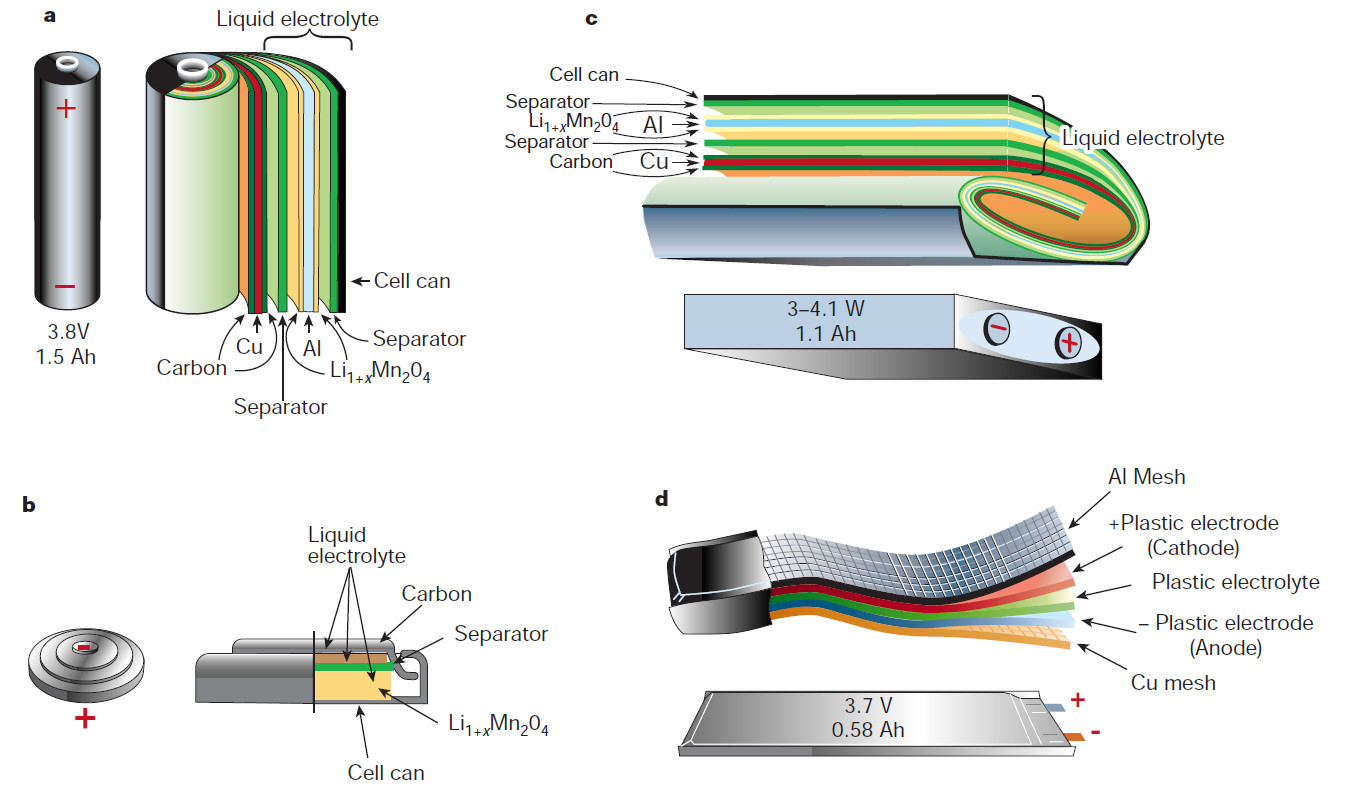
\includegraphics[width=1.0\columnwidth]{images/uebersicht_bauformen.jpg}
	\caption{Vergleich möglicher Bauformen: (a) Rundzelle, (b) prismatische Zelle, (c) Knopfzelle, (d) Pouch-Zelle \cite{tarascon2001issues}}
	\label{vergleich_zellform}
\end{figure}
\begin{figure}
	\centering
	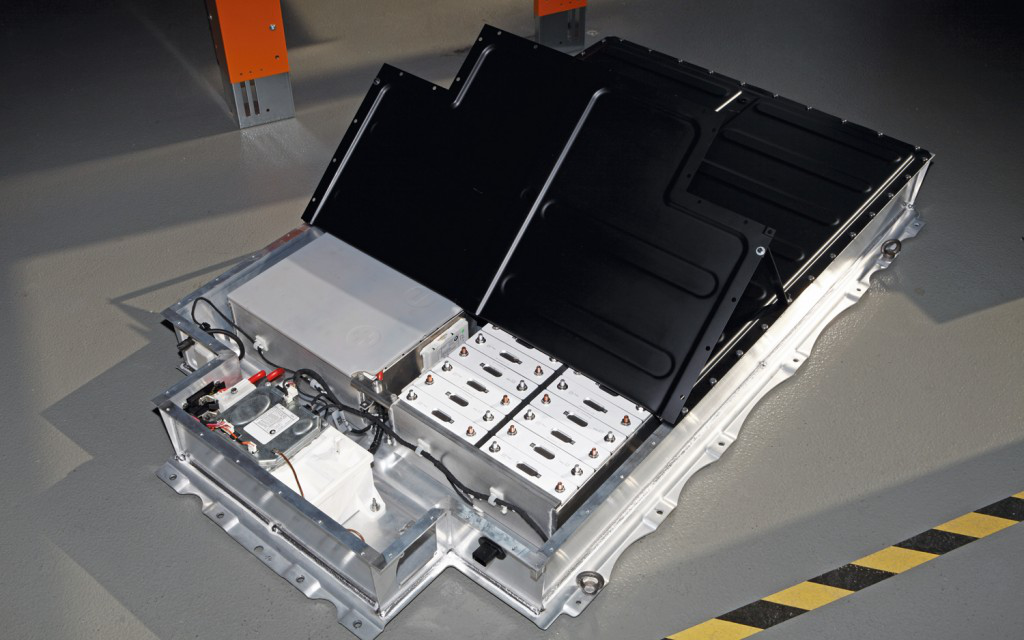
\includegraphics[width=0.9\columnwidth]{images/bmw-i3-battery-pack.png}
	\caption{Battery-Pack des BMW i3 bestehend aus zwei Batteriemodulen und einem Batteriemanagement \cite{bmwblog}}
	\label{battery_pack}
\end{figure}
\begin{description}
\item[Rundzellen] Bei der Rundzellen werden die Stromkollektoren jeweils doppelseitig mit einem Elektrodenmaterial beschichtet und dann abwechselnd aufeinander gestapelt. Anschließend wird die Batteriezelle zu einem Zylinder aufgewickelt.
\item[Prismatische Zellen] Die prismatische Zelle ähnelt im Aufbau der Rundzelle, wird jedoch rechteckig gewickelt und ist so besser schichtbar.
\item[Pouch-Zellen] In diesen Zellen werden meist nur wenige Schichten von Elektroden übereinander gewickelt und anschließend in einer dünnen Hülle gasdicht verschweißt. Ein vor dem Einschweißen durchgeführtes Anbringen eines Vakuums garantiert das Entfernen überflüssiger Gase innerhalb der Zelle.
\item[Knopfzellen] In einer Knopfzelle werden die Elektroden, Elektrolyt und Separator jeweils rund geformt auf einem Boden gestapelt und anschließend mit einem Deckel verschlossen. Eine zusätzlich eingebrachte Feder zwischen Zelle und Deckel sorgt für den notwendigen Anpressdruck, um eine gute Kontaktierung zu gewährleisten.
\end{description}
Eine Übersicht über die verschiedenen Bauformen wird in Abbildung \ref{vergleich_zellform} gezeigt. Batteriezellen können zu Batteriemodulen zusammengeschlossen werden, die dann über ein externes Batteriemanagement gezielt angesprochen und kontrolliert werden können. Ein solcher Aufbau ist in Abbildung \ref{battery_pack} zu sehen.
\\\\
Am IAM-KWT kommen spezielle Testzellen zum Einsatz, deren Aufbau dem von Knopfzellen ähnelt. Die beiden Elektroden und der Elektrolyt werden in eine Glasröhre übereinander montiert. Die Röhre ist über zwei Edelstahlstopfen mit Dichtungsringen nach außen hin abgedichtet. Eine Druckfeder sorgt für den nötigen Anpressdruck, zwei Edelstahlplättchen für eine homogene Kraftverteilung und Kontaktierung. Verschlossen wird die Zelle mittels Plastikverschlüssen, welche die Stopfen am Verrutschen hindern. Über einfache 2mm-Bohrungen in den Stopfen kann die Zelle mit Bananensteckern an Geräte angeschlossen werden. Die Abbildung \ref{schema_zelle} zeigt die Testzelle schematisch.
\begin{figure}
	\centering
	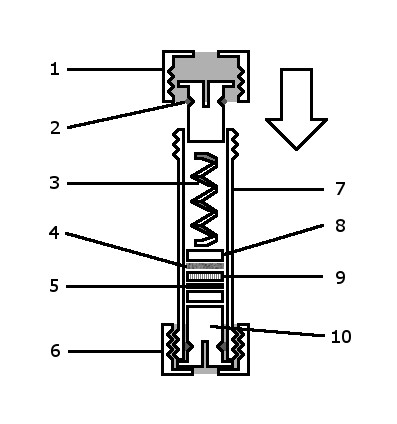
\includegraphics[width=0.55\columnwidth]{images/Schema_Zelle.jpg}
	\caption{Schema der IAM-KWT-Testzelle; 
			1: Plastikkappe,
			2: Dichtungsring,
			3: Edelstahlfeder,
			4: Kathode,
			5: Anode,
			6: Plastikkappe,
			7: Glaszylinder,
			8: Kontaktierplättchen,
			9: Separator,
			10: Edelstahlstopfen.
			}
	\label{schema_zelle}
\end{figure}
\section{Anforderungen an die in-situ Testzelle}
Ziel ist die Konstruktion einer Testzelle, in welcher sowohl herkömmliche Batterien als auch Festkörperelektrolyt-Batterien eingebaut werden können. Für den Einsatz von reinem Lithium\-metall und Flüssigelektrolyten muss die Testzelle gasdicht gebaut werden können. Die eingesetzten Materialien müssen alle ausreichend amagnetisch sein, um die empfindlichen Kernspinresonanzmessungen der NMR-Spektroskopie nicht zu sehr zu stören. Sie sollte möglichst ähnlich wie die bereits am IAM-KWT im Einsatz befindliche Zelle aufgebaut sein, um eine Vergleichbarkeit zwischen beiden Zellen zu gewährleisten und einen Einsatz auch außerhalb der NMR-Anlage zu ermöglichen. 
\\\\
Der Außendurchmesser der Zelle ist durch den Aufbau des NMR-Probenkopfes auf maximal 10mm festgesetzt. Eine Ausnahme stellt hier der Zellabschluss dar, da dieser über die Teflonhülle der Spule des Probenkopfes reichen kann und daher lediglich durch die Öffnung der Kupferabschirmung des Probenkopfes beschränkt ist. Diese hat einen Durchmesser von 16,5mm. Der relevante Messbereich der Spule befindet sich auf einer Höhe von 22mm bis 32mm. Ein Anschluss an den externen Stromkreis zum Laden und Entladen der Zelle kann nur nach oben hin erfolgen.
\\\\
In der Literatur lassen sich unterschiedliche Umsetzungen von in-situ-Testzellen für NMR-Spektroskopie finden. Die Arbeitsgruppe von Silvio Indris am IAM-ESS sowie Zhou et al. \cite{zhou2013paramagnetic} und Key et al. \cite{key2009real} benutzen dafür Pouch-Zellen, die gerollt oder gefaltet in den NMR-Aufbau eingebracht werden können. Dies ist jedoch mit Festkörperelektrolyten wegen des starren Aufbaus der Zelle nicht möglich, weshalb dieser Ansatz nicht verfolgt wurde.  Poli et al. \cite{poli2011new} und Gerald et al. \cite{gerald2001situ} implementieren beide einen Knopfzellenaufbau. Beide Lösungen sehen aber einen umfangreichen Umbau des NMR-Probenkopfes vor. Die angestrebte Lösung soll jedoch eine weitere Verwendung des Probenkopfes für andere NMR-Experimente im gewohnten Messaufbau und damit einhergehend schnelles Umrüsten des Probenkopfes ermöglichen.
\section{Planung und Anfertigung der Teile}
\begin{figure}
	\centering
	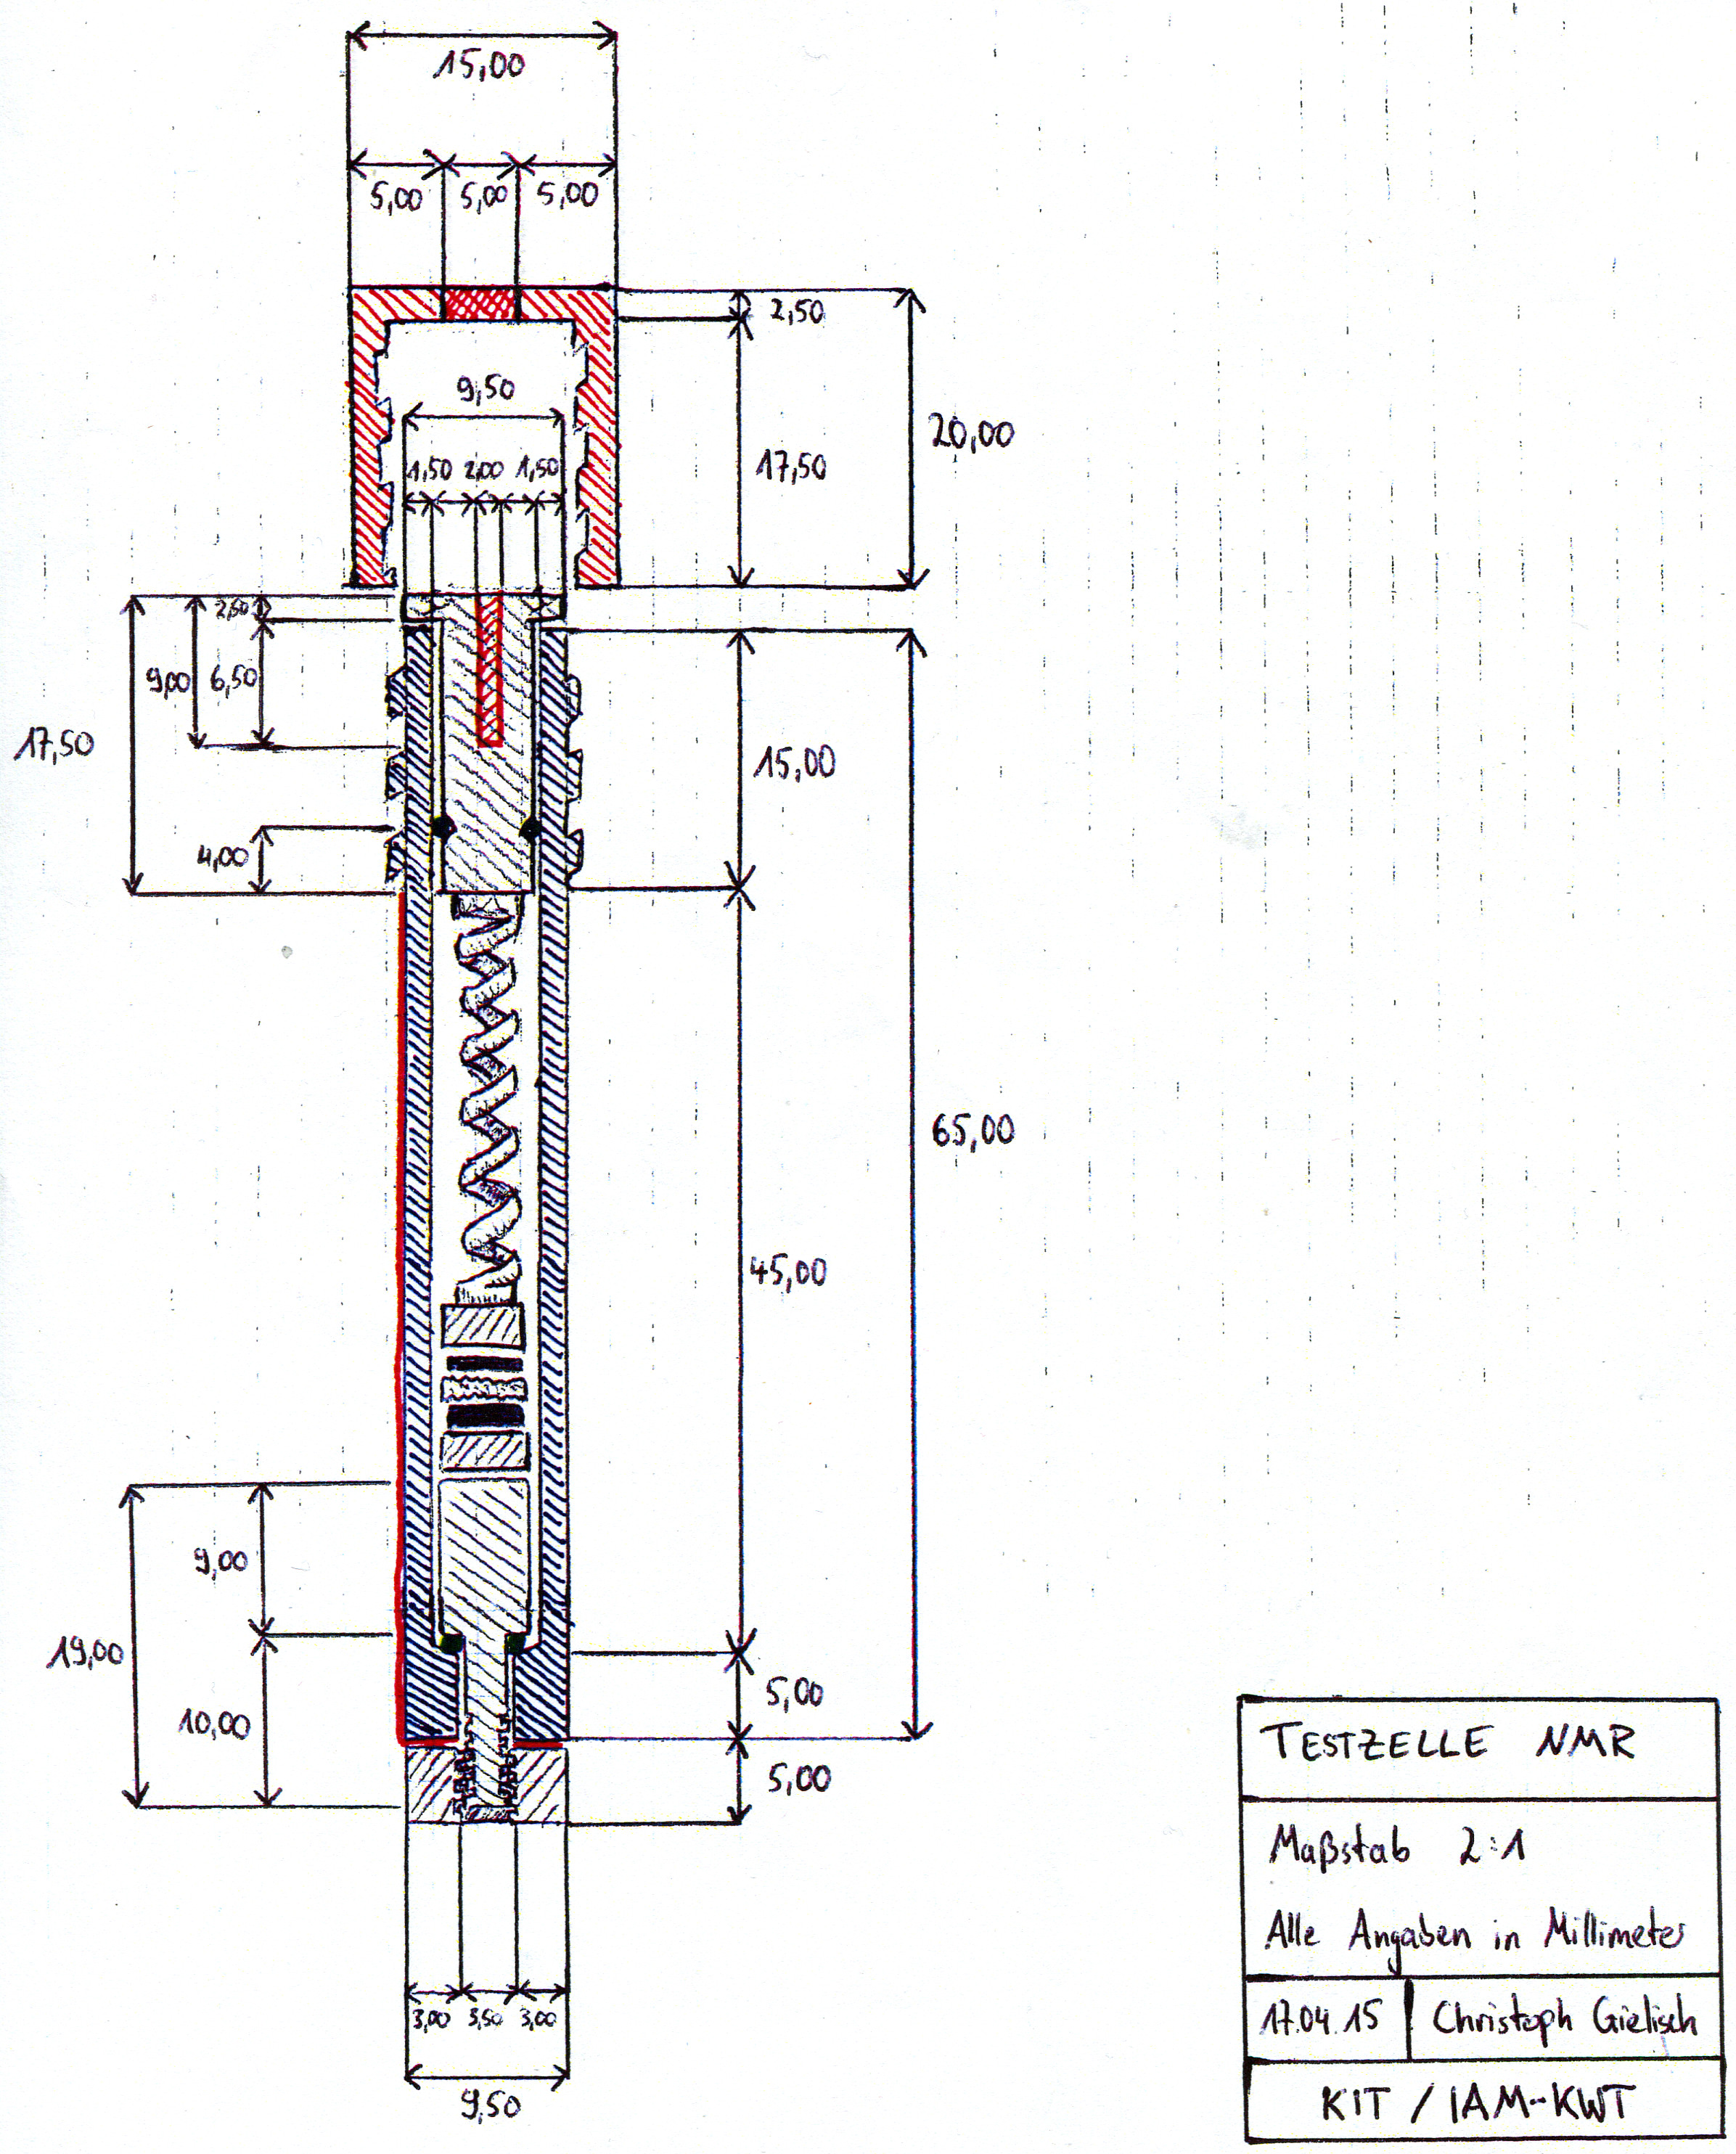
\includegraphics[width=1.0\columnwidth]{images/Skizze_Testzelle.jpg}
	\caption{Skizze der Testzelle}
	\label{skizze_testzelle}
\end{figure}
Der Aufbau des NMR-Spektrometers gibt eine zylindrische Form der einzuführenden Probe vor. Da die gewickelte Zellen für Festkörperelektrolytbatterien nicht geeignet sind, wird ein Knopfzellenaufbau gewählt. Für die einfachere Handhabung wird ein länglicheres Design mit einer normalen Druckfeder, ähnlich der bereits am IAM-KWT im Einsatz befindlichen Testzelle, umgesetzt. Jedoch musste der bisherige Abschluss der Zelle umgestaltet werden. Um in den Probenkopf eingeführt werden zu können, muss der Boden der neuen Zelle bündig mit der restlichen Zelle abschließen und darf nicht auskragen. Dies würde den optimalen Sitz der Spule verhindern. Der Verschluss kann daher nicht außenliegend erfolgen. Die Kontaktierung kann nicht nach unten hinweg erfolgen, weshalb an der Außenseite der Zelle nach oben hin eine Leitung existieren muss. Beide Maßnahmen erfordern ein neues Design des unteren Stempels sowie der äußeren Hülle. Der obere Stempel und die Feder müssen sowohl auf den kleineren Durchmesser hin angepasst werden, als auch aus amagnetischen Materialien gefertigt werden. Abbildung \ref{skizze_testzelle} zeigt skizzenhaft die Planung der neuen Testzelle.
\subsection{Die Glaszelle}
Als Material für die Zellhülle wurde Glas ausgewählt. Glas bietet den Vorteil einer optischen Kontrolle der Zelle während des manuellen Einbaus der verschiedenen Komponenten. Es ist auch bei dünnen Wandstärken ausreichend fest, womit der Innendurchmesser maximiert werden konnte. Glas ist ausreichend amagnetisch und kann gut bearbeitet werden.
\\\\
Die Glaszelle wurde von einem Glasbläser der Laborhandelsgesellschaft GmbH (Karlsruhe) aus einem Glasrohr gefertigt, welches unten nach innen verdickt und durchstochen worden ist und an das nach oben mit einem Standardgewindeteil (GL14) versehen worden ist.
\\\\
Die mitgelieferten Plastikdeckel mussten auf den maximalen Durchmesser der Kupferabschirmung von 16,5mm abgeschliffen werden. Dies erfolgte händisch auf einer Schleifmaschine des Typs DAP-V der Firma Struers.
\subsection{Die Stempel}
Die beiden Stempel wurden jeweils als CAD-Modell mit der Software Creo Parametric der Firma PTV geplant. Die Zeichnungen sind in Abbildung \ref{stempel_oben} und \ref{stempel_unten} dargestellt. Der obere Stempel entspricht dabei dem Stempel aus der existierenden Zelle mit angepasster Höhe, Durchmesser und Nut für den Dichtungsring. Die 2mm-Bohrung zur Kontaktierung bleibt erhalten. Der untere Stempel wurde komplett neu gestaltet. Er besteht aus einem Kopf mit einer Nut für den Dichtungsring, welcher für die Dichtigkeit der Zelle sorgt. Von ihm abgehend ist ein Stab mit einem M3-Isogewinde. Dieser passt durch die Aussparung der Glaszelle und ermöglicht das Befestigen des Stempels mit einer außenliegenden Mutter. Als Material kommt eine Messinglegierung zum Einsatz (\ce{CuZn39Pb3}), welche ausreichend amagnetisch (Suszeptibilität X $=\;-$0,173 · 10$^{-6}$ cm$^3$/g) ist. 
\\\\
Die Stempel wurden an einer CNC-Drehmaschine von Technikern der Technologiefabrik Karlsruhe gedreht. %Typ der Drehmaschine?
\begin{figure}
%mit Subfigures machen?
	\centering
	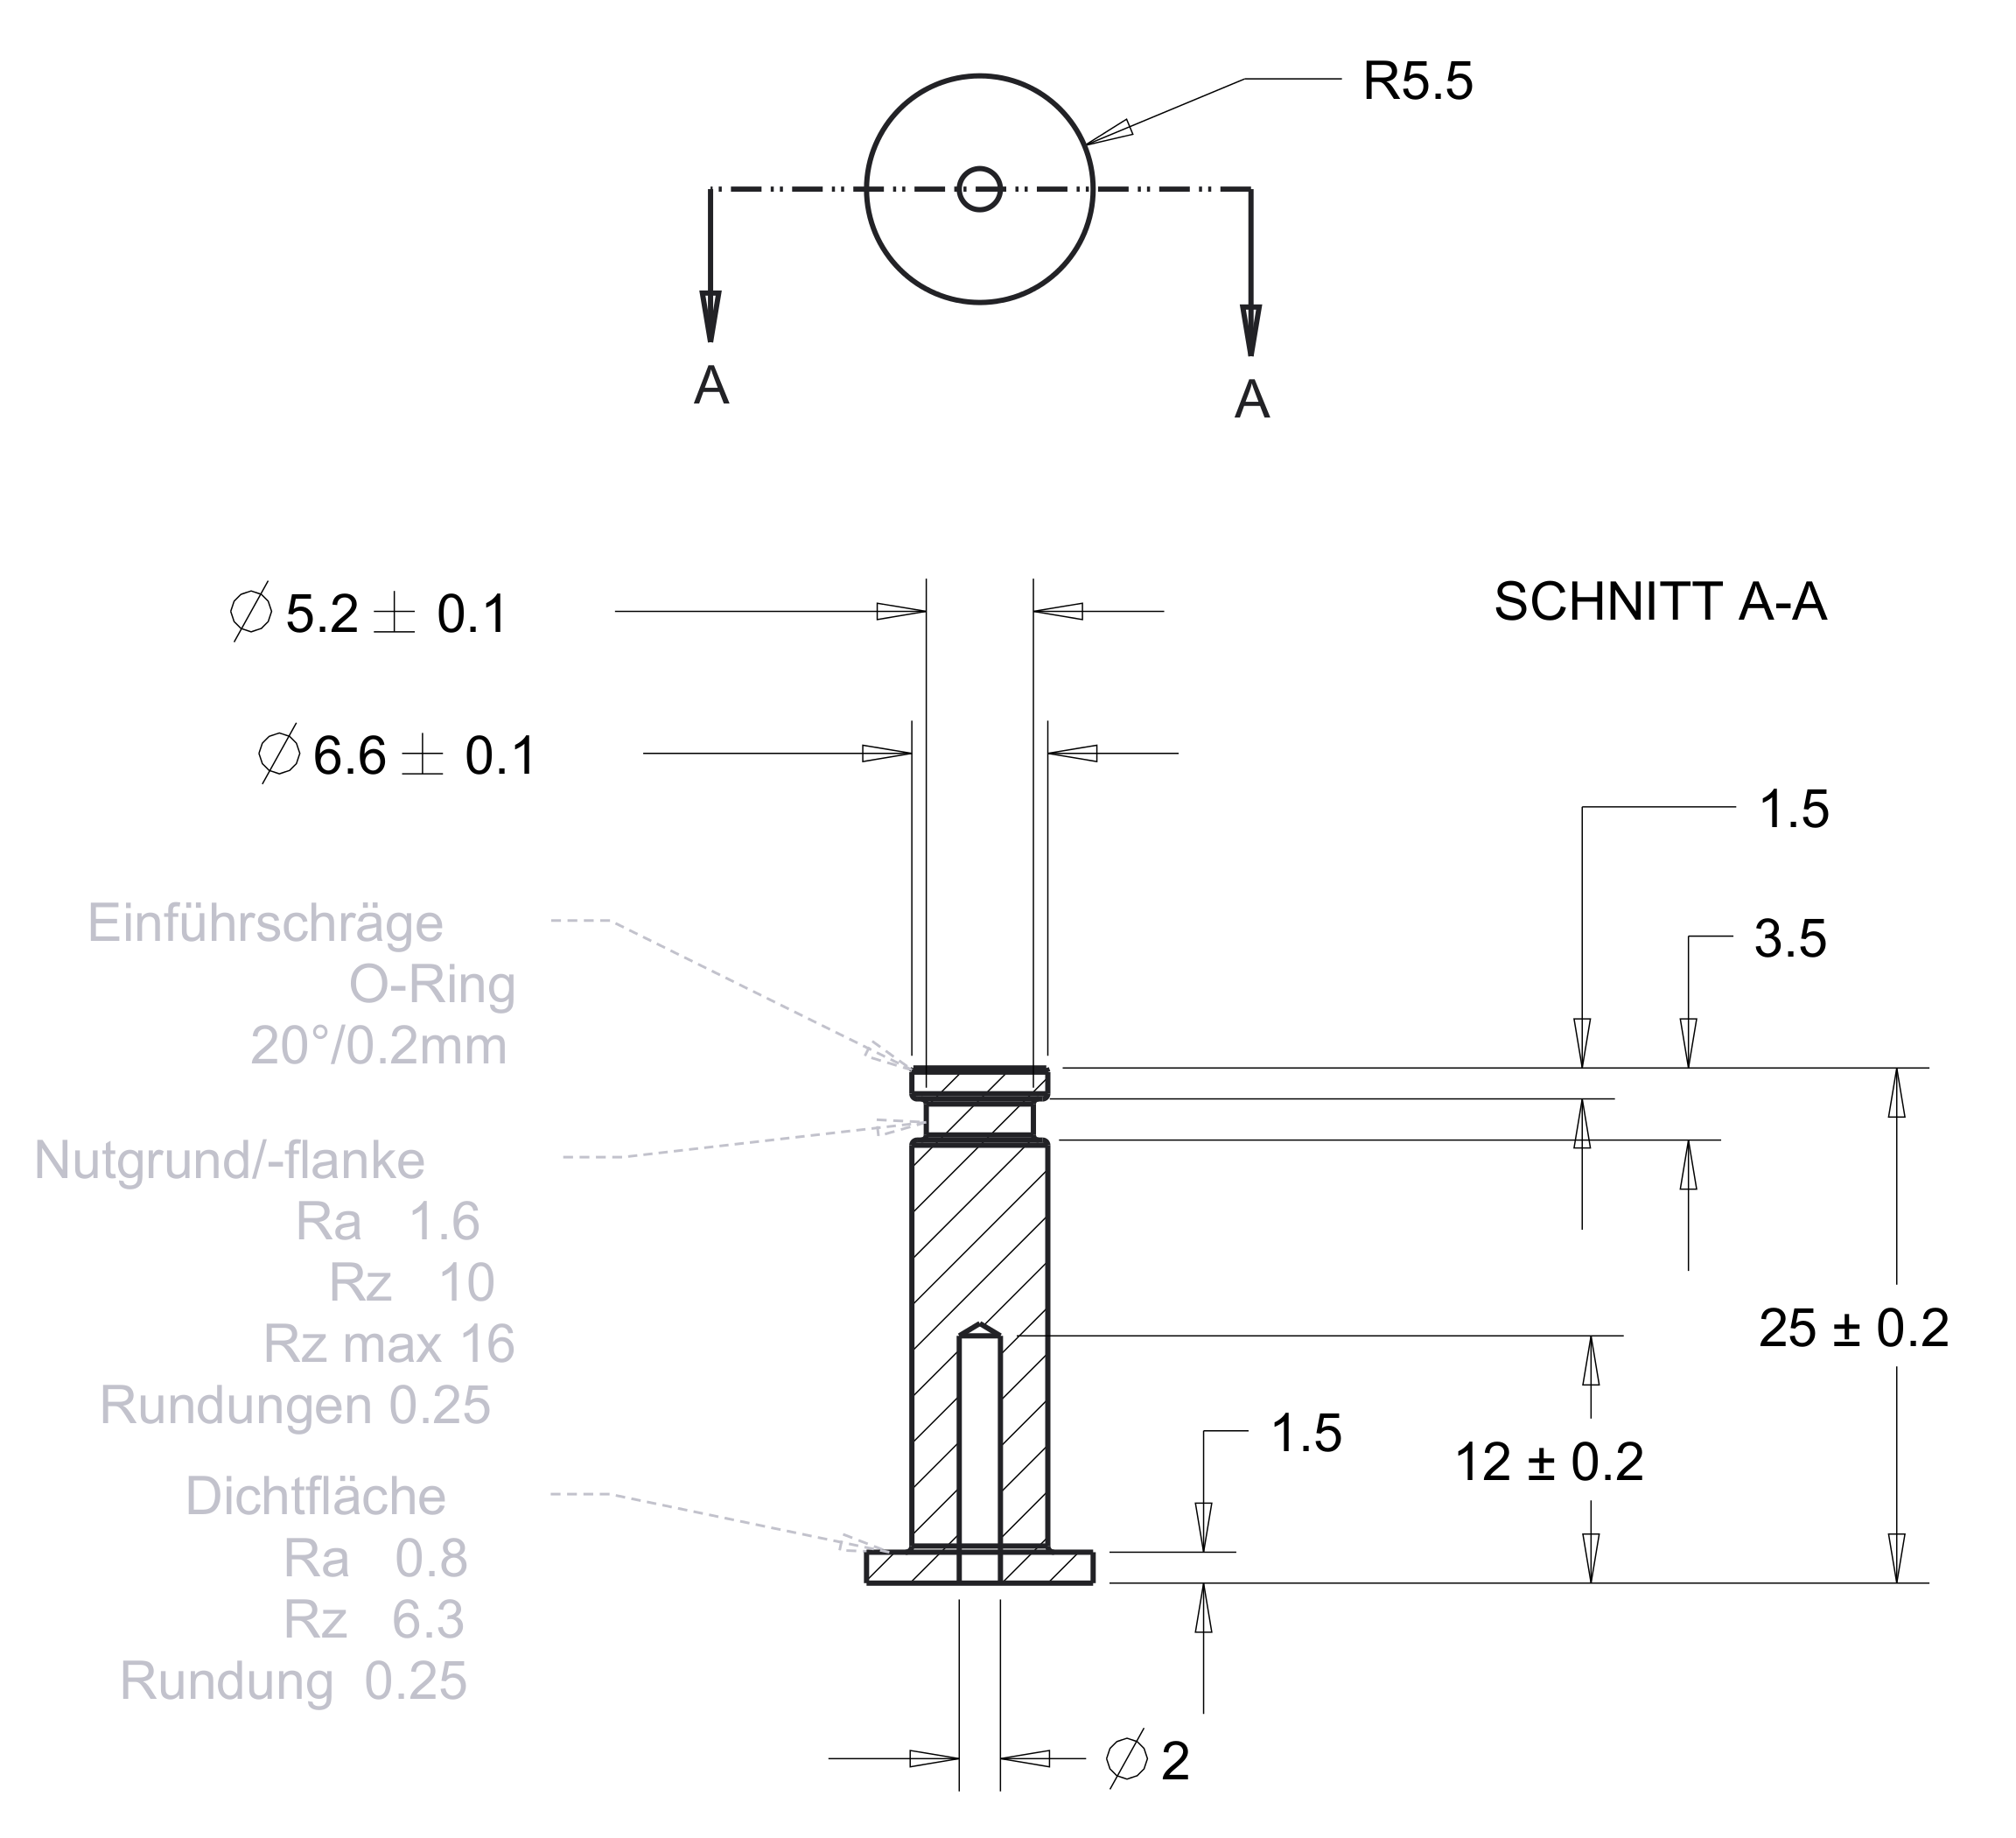
\includegraphics[width=0.7\columnwidth]{images/stempel_oben.png}
	\caption{Stempel oben}
	\label{stempel_oben}
\end{figure}
\begin{figure}
	\centering
	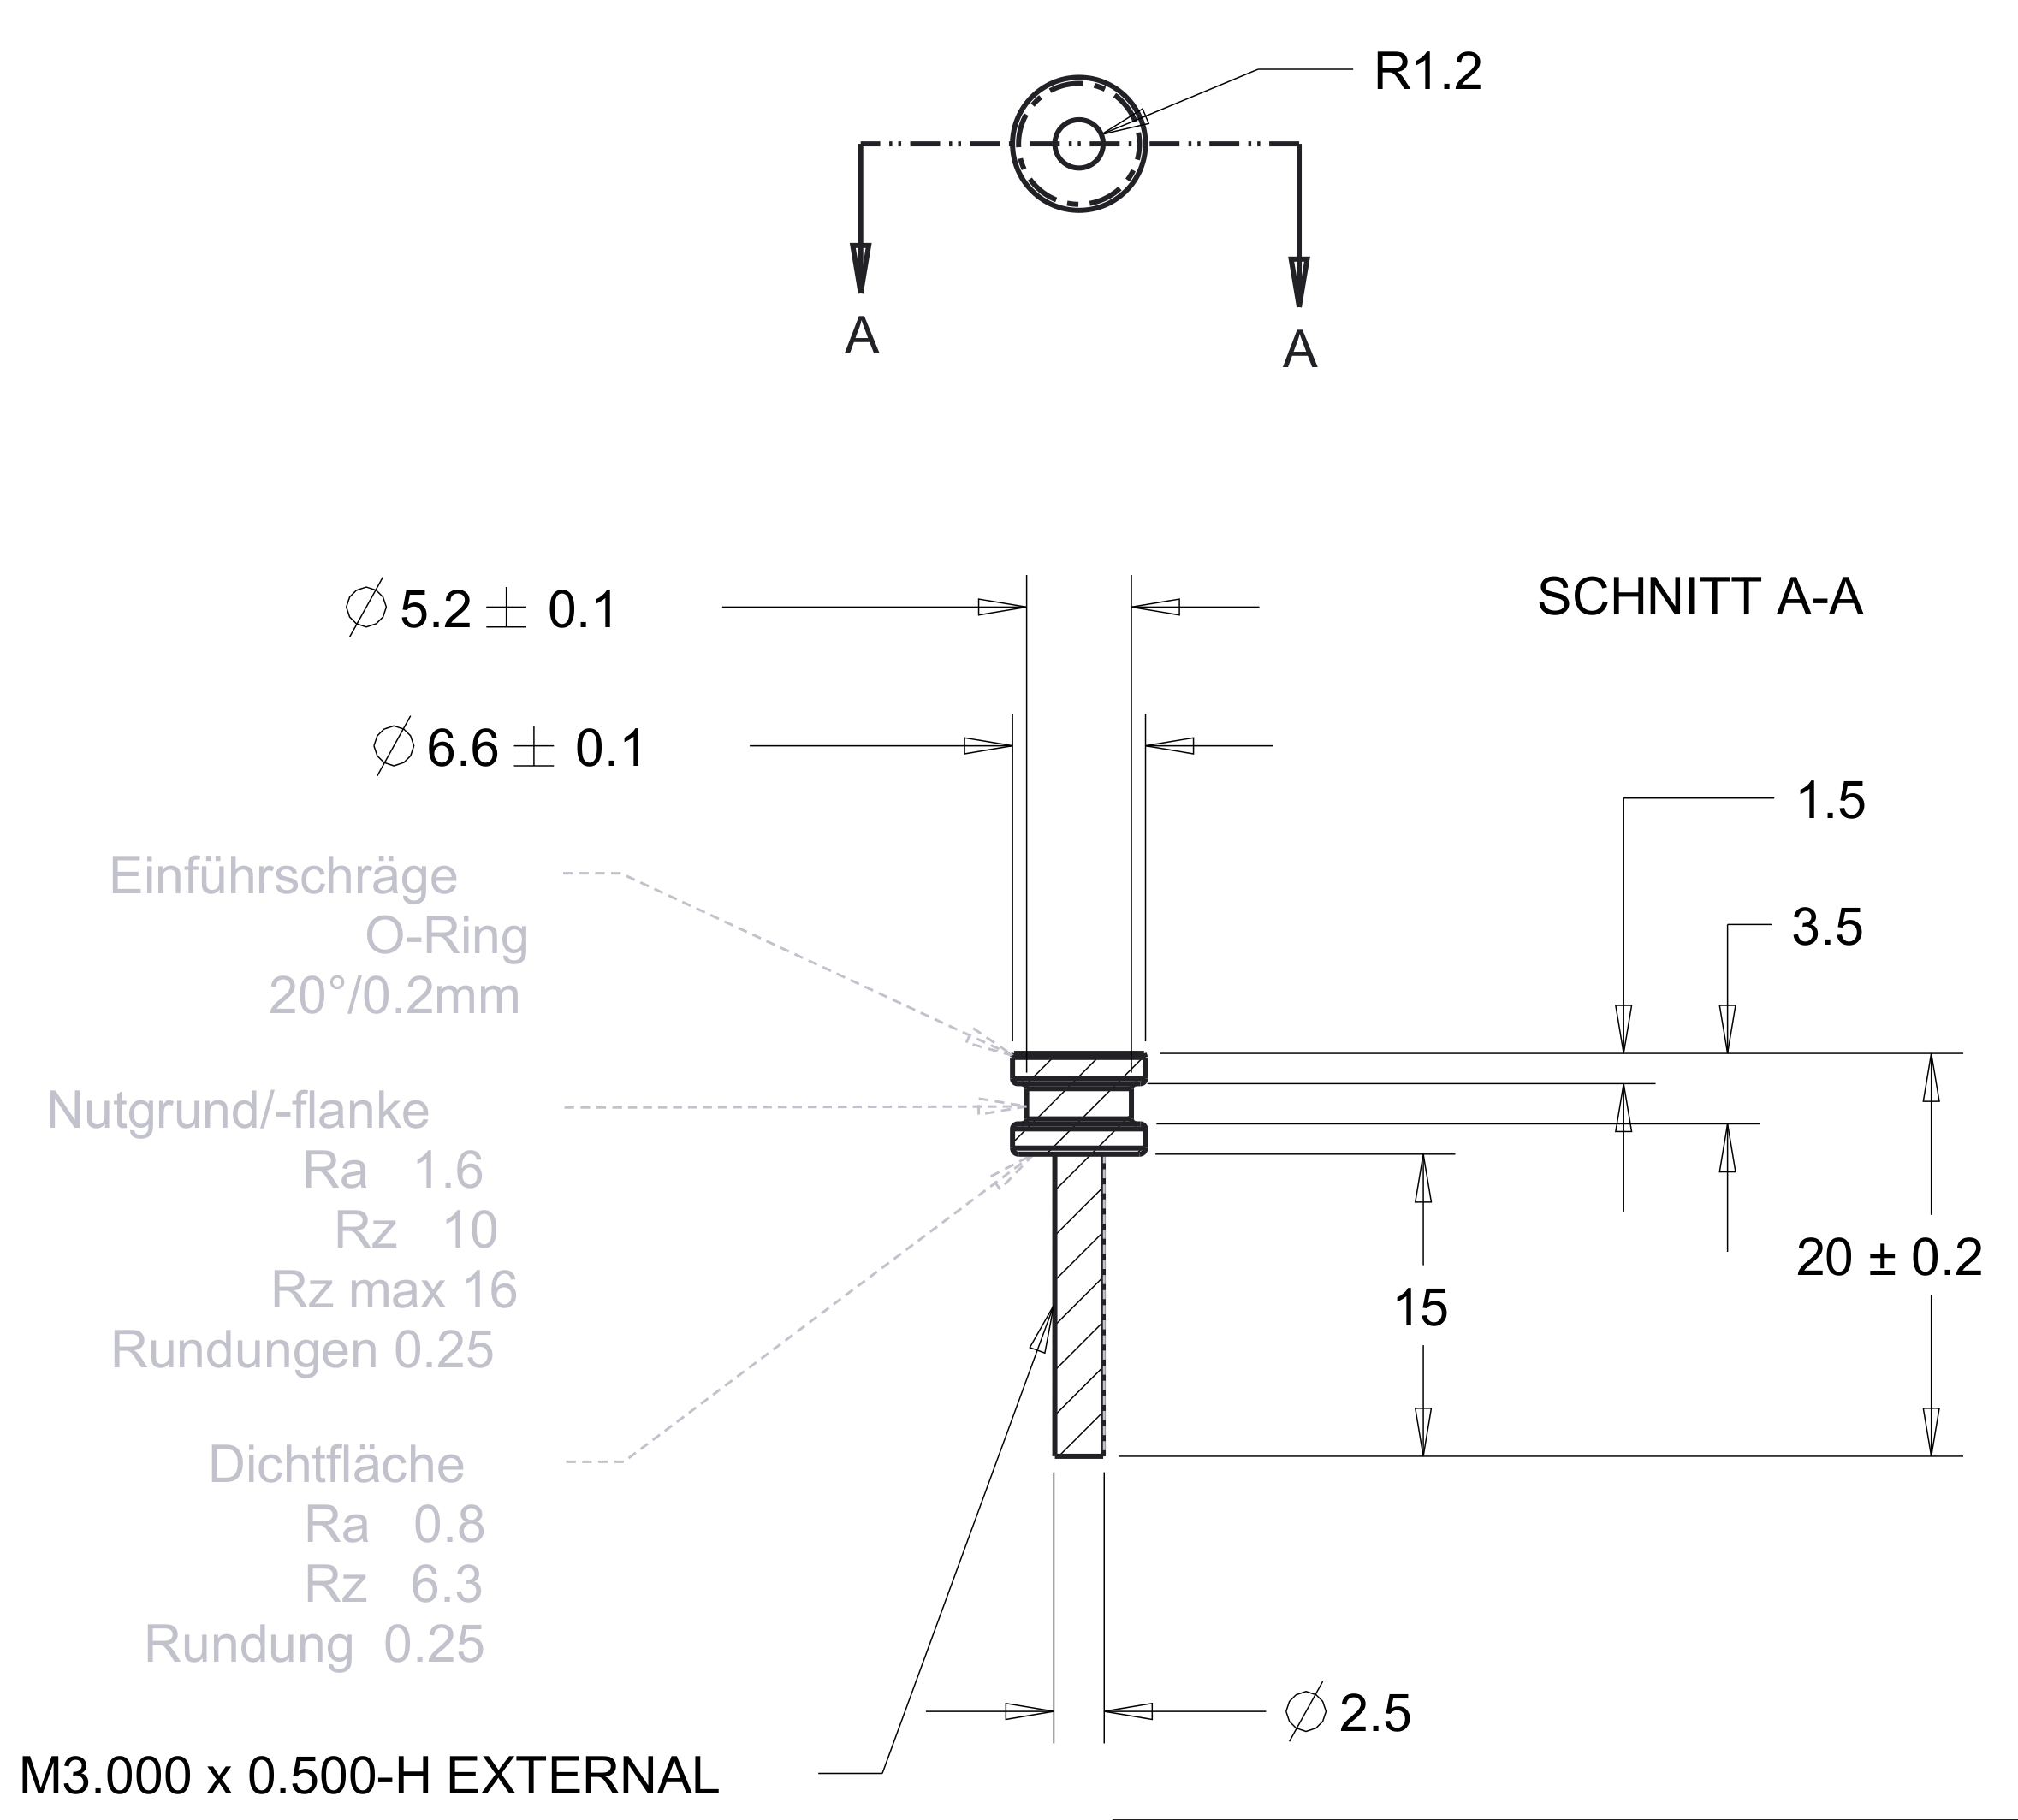
\includegraphics[width=0.7\columnwidth]{images/stempel_unten.png}
	\caption{Stempel unten}
	\label{stempel_unten}
\end{figure}
\begin{figure}
	\centering
	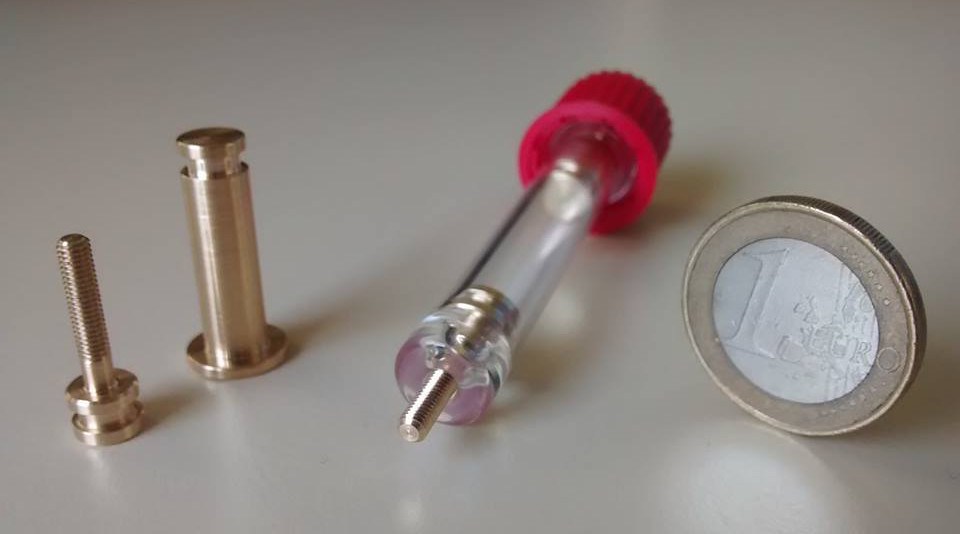
\includegraphics[width=1.0\columnwidth]{images/Stempel_Foto_cutted.jpg}
	\caption{Übersicht über die verschiedenen Teile des in-situ-Testzelle (besseres Foto machen!)}
	\label{uebersicht_teile}
\end{figure}
\subsection{Die Mutter}
Durch den Einsatz des M3-Standardgewindes bei den Stempeln, konnte bei der Mutter ein Standardmodell aus Messing aus dem Fachhandel eingesetzt werden.
\subsection{Die Feder}
Die Feder stellte besondere Herausforderungen an die Materialauswahl. So musste neben der amagnetischen Eigenschaft auch eine gute elastische Verformbarkeit und eine gute Leitfähigkeit für den elektrischen Strom gegeben sein. Neben Messing wurde daher auch Federbronze (\ce{CuSn6}) und Kupferberyllium (\ce{CuBe2}) als mögliche Materialien betrachtet.
% Tabelle mit Übersicht?
\\\\
Die Feder wird dabei so ausgelegt, dass der Anpressdruck auf die Zelle möglichst gleich ist, wie bei der bereits am IAM-KWT existierenden Zelle. Diese baut bei einem Federweg von 25 mm und einer Federrate von 0,541 N/mm eine Kraft von 13,525 N auf. Bei einer Fläche von 93,3 mm$^2$ entspricht dies einem Anpressdruck von 0,145 N/mm$^2$. Die Höhe der neuen Feder wurde auf 30 mm festgelegt, der zu absolvierende Federweg bei Einbau beträgt 10 mm. Die Fläche auf der die Kraft aufgebracht wird beträgt 36,32 mm$^2$. Um den gleichen Anpressdruck zu gewährleisten, benötigt die neue Feder daher eine Kraft von 5,266 N, was einer Federrate von 0,527 N/mm entspricht.
\\\\
Die Feder wurde von Febrotec Federn (Halver) aus Kupferberyllium gefertigt. Der Drahtdurchmesser beträgt 0,75 mm, der Federnaußendurchmesser 6,5 mm. Ungespannt hat die Feder eine Höhe von 30mm. Die Zahl an Windungen beträgt 20, die Enden der Feder sind angelegt und geschliffen. % Federrate?
\subsection{Die Positionsplättchen}
Die Positionsplättchen sorgen dafür, dass sich die eigentliche Batteriezelle, also die Elektroden und der Elektrolyt, im sensitiven Bereich der Spule befindet. Da sie sich selbst dadurch unmittelbar im Messbereich aufhalten, wird auf eine vollständige Metallfertigung verzichtet, um die dämpfende Wirkung zu minimieren. Stattdessen werden von einem Teflonstab passende Scheiben abgeschnitten und plan geschliffen. Anschließend werden die beiden Grundflächen mit Kupferklebeband abgeklebt. Die beiden Seiten sind über einen dünnen Kupferstreifen an der Seite miteinander verbunden. 
\\\\
Eine Übersicht über alle konstruierten und gebauten Teile der in-situ NMR-Batterietestzelle findet sich in Abbildung \ref{uebersicht_teile}.
\section{Anpassung des NMR-Probenkopfes}
\label{anpassung_probenkopf}
\begin{figure}
	\centering
	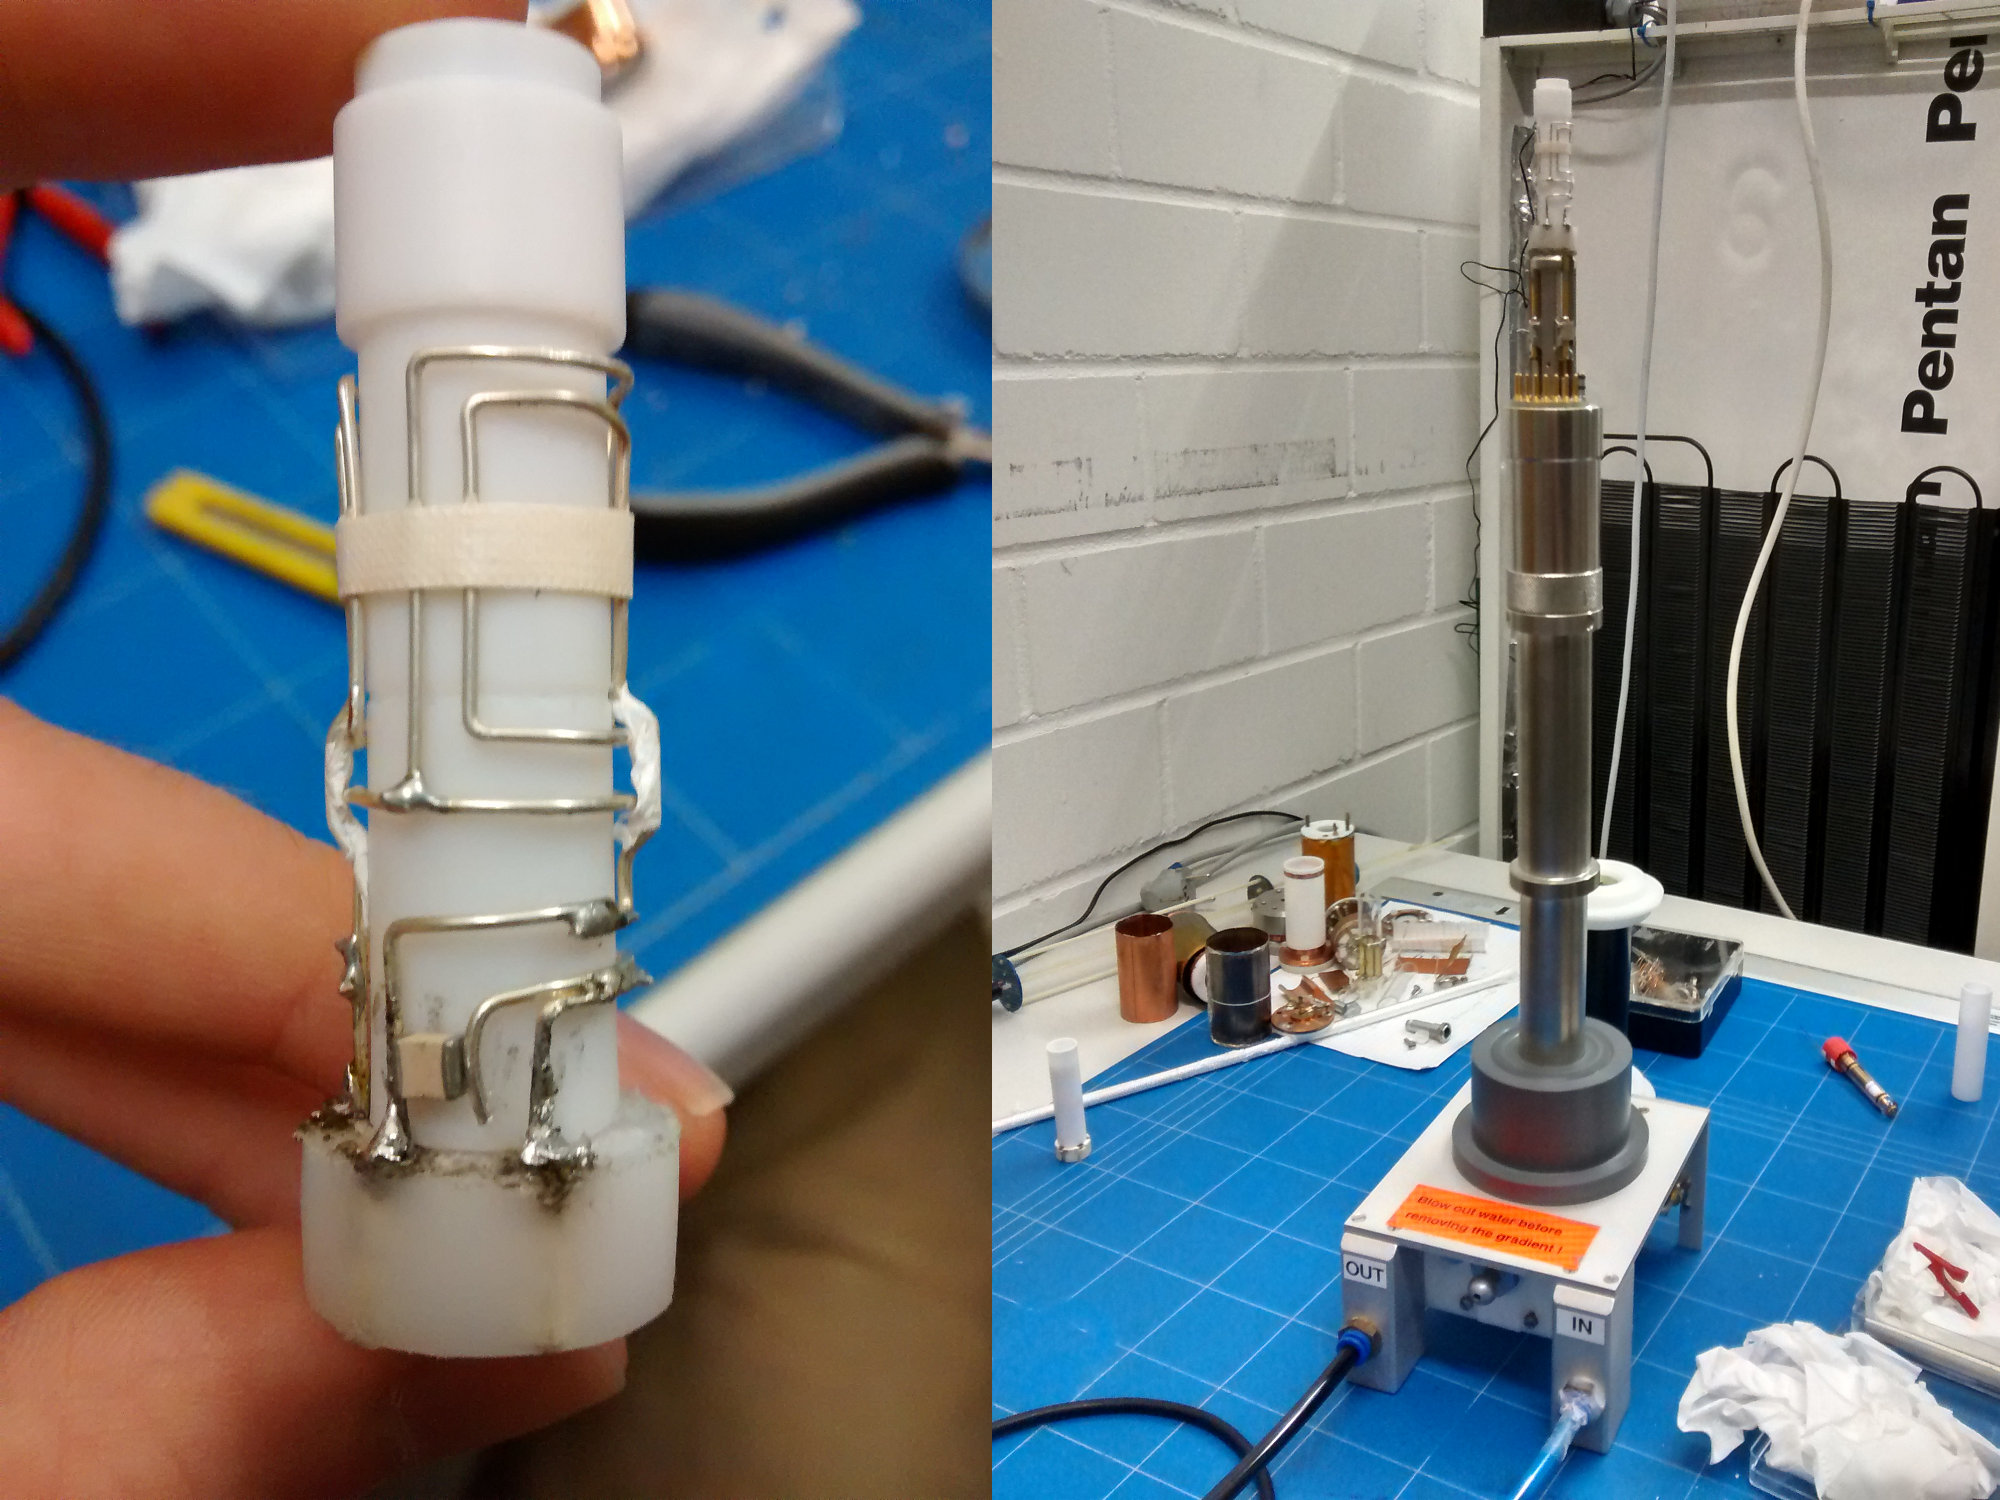
\includegraphics[width=0.85\columnwidth]{images/Platzhalter_Spule.jpg}
	\caption{Spule mit Kondensator (links) und eingebaut in den Probenkopf (rechts)}
	\label{spule}
\end{figure}
Die in-situ-Testzelle kommt im 200MHz-NMR-Spektrometer der Firma Bruker am Institut für Mechanische Verfahrenstechnik und Mechanik (MVM) zum Einsatz. Dafür wurde der Probenkopf entsprechend angepasst. Es wurde eine neue Sattelspule um ein Teflonrohr mit Innendurchmesser von 10mm gewickelt. Diese musste anschließend mit dem Anschlussstempel des Probenkopfes verlötet werden. Damit die Spule auf der richtigen Resonanzfrequenz von 77,7MHz für Li$^7$-NMR arbeitet, wurde ein 5pF-Kondensator in den Spulen-Schwingkreis eingebaut. Die Spule und der Probenkopf werden in Abbildung \ref{spule} dargestellt. Um einen Kurzschluss der Spule durch die massive Kupferabschirmung nach außen hin zu vermeiden, wird eine zweite Teflonröhre über die Spule gestülpt.

%%%%%%%%%%%%%%%%% 4. PROBENPRÄPERATION %%%%%%%%%%%%%%%%%

\chapter{Probenpräperation}
Zuerst wird die Herstellung der in Kapitel \ref{grundlagen_keramik} vorgestellten NASICON-Keramiken LATP und LAGP sowie des Perowskiten LLTO beschrieben. Zusätzlich wird das Standardelektrodenmaterial LTO sowie zu Zwecken der Charakterisierung auch die im LATP häufig vorkommende Fremdphase \ce{LiTiPO5} in Reinfrom hergestellt. Anschließend erfolgt die Beschreibung der Mischung der Keramiken zu Elektrodensuspensionen und der Folienguss dieser. Im dritten Abschnitt wird die Konstruktion und der Bau einer neuen in-situ NMR-Testzelle beschrieben. Im letzten Abschnitt wird der Bau der unterschiedlichen Batterie-Testzellen aus den Elektrodenfolien dargestellt. 
\section{Pulverherstellung}
Die Herstellung der Pulver erfolgte bei LATP, LAGP und dem \ce{LiTiPO5} mit dem patentierten Sol-Gel-Verfahren des IAM-KWT. Für die beiden Perowskite LTO und LLTO wurde ein Mischoxiod-Verfahren ausgewählt.
\subsection{Herstellung des LATP-Pulvers}
\label{praep_LATP}
Bei der Herstellung des LATP kommt das Sol-Gel-Verfahren zum Einsatz. Als Ausgangsmaterial werden drei Stoffe verwendet: Aluminiumnitrat (\ce{Al(No3)3 \; 9H2O}, EMSURE), Lithiumacetat (\ce{LiCOOCH3 \; 2H2O}, Reagent Grade, Alfa Aesar) und Tetra\-iso\-propyl\-ortho\-titanat (\ce{C12H28O4Ti}, Merck). Die Einwaage der Stoffe erfolgt stöchiometrisch. Alle werden jeweils in Wasser gelöst und anschließend miteinander vermengt. Danach wird Phosphorsäure (\ce{H3PO4}, Merck) zugegeben. Auf Grund der dabei entstehenden Reaktionswärme erfolgt dies in einem Wasserbad unter kontinuierlichen Rühren.
\\\\
Um die organischen Anteile des Gels zu entfernen, wird dieses zunächst für acht Stunden bei 400$^\circ$C wärmebehandelt. In einem zweiten Schritt kann dann mit einem weiteren Glühschritt bei 900$^\circ$C für acht Stunden die gewünschte LATP-Struktur erzeugt werden. Um feinere Agglomerate zu erhalten wird das Pulver noch mit einem Mörser zerkleinert.
% Hinweis auf Paul?
\subsection{Herstellung des LAGP-Pulvers}
\label{praep_LAGP}
Die Herstellung von LAGP erfolgt ebenfalls über den Sol-Gel-Prozess, der auch schon bei LATP angewendet wurde. Anstatt Titanphosphat wird Germaniumoxid ($>99\%$, Aldrich) verwendet. Dieses bildet mit Wasser allerdings keine homogene Lösung, weshalb der Ansatz mittels kontinuierlichem Rühren am Sedimentieren gehindert werden muss. Überschüssiges Wasser wird noch vor dem Kalzinierschritt verdampft.
\subsection{Herstellung des LLTO-Pulvers}
\label{praep_LTO}
Bei der Herstellung des LTO kommt ein Mischoxid-Prozess zum Einsatz. Lithiumcarbonat (\ce{Li2CO3}, 99,998\%, Alfa Aesar) und Titandioxid (\ce{TiO2}, Titanium(IV) oxide, $>99.9\%$, Aldrich) werden in Isopropanol dispergiert und in einem Attritor deagglomeriert sowie homogenisiert. Das Isopropanol wird mit einem Rotationsverdampfer und mit einer eintägigen Lagerung in einem Vakuumtrockenschrank bei 60$^\circ$C entfernt. Als letzter Schritt wird das Pulver bei 800$^\circ$C für 12 Stunden kalziniert.
\subsection{Herstellung des LTO-Pulvers}
\label{praep_LLTO}
Die Herstellung von LLTO erfolgt analog zu der des LTO. Es wird jedoch noch zusätzlich Lanthanoxid (\ce{La3O2}, 99,99\%, Aldrich) mit in Isopropanol dispergiert. Weiterhin wird ein Lanthanüberschuss von 2,5 m\% vorgelegt. Die Kalzinierung findet für acht Stunden bei 950$^\circ$C statt.
\subsection{Herstellung des \ce{LiTiPO5}-Pulvers}
\label{praep_LiTiPO5}
\begin{figure}
	\centering
	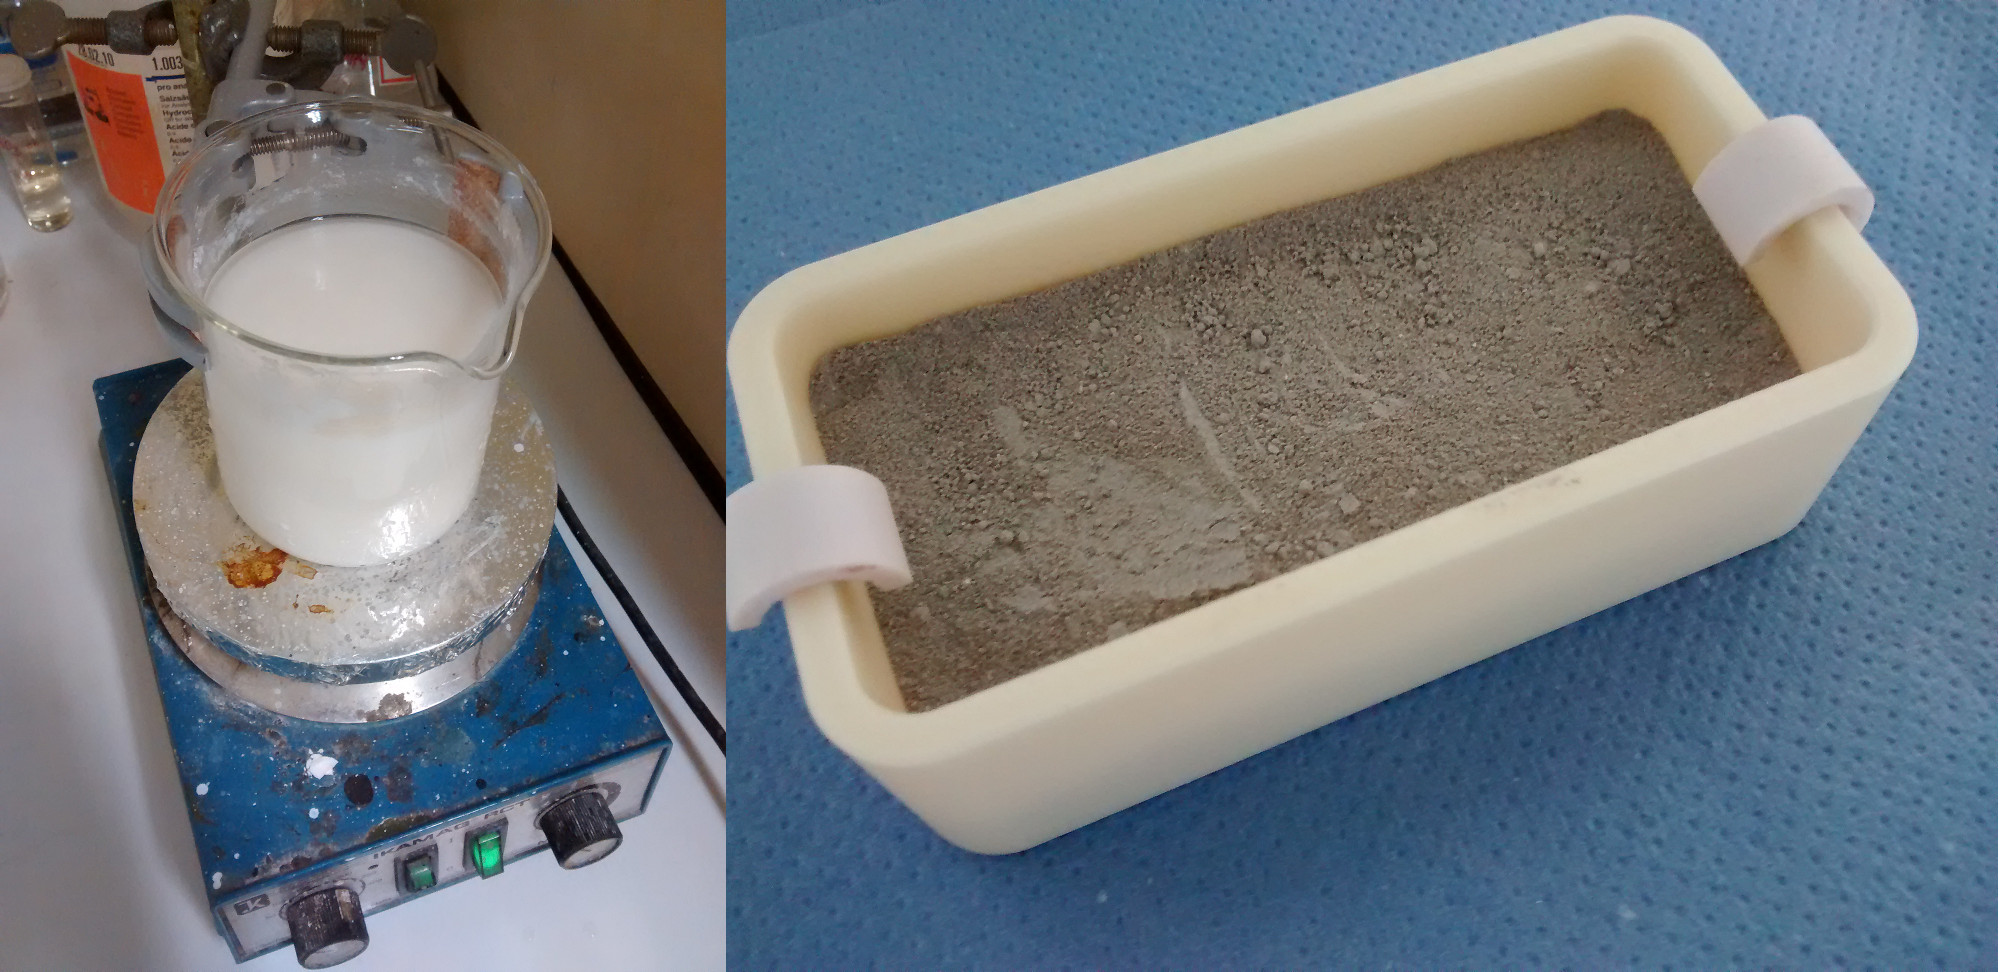
\includegraphics[width=1.0\columnwidth]{images/SolGel.jpg}
	\caption{Herstellung von \ce{LiTiPO5} über einen Sol-Gel-Prozess}
	\label{sol_gel}
\end{figure}
Die Herstellung des \ce{LiTiPO5} erfolgt analog zur Herstellung des LATP im Sol-Gel-Verfahren. Es wird jedoch auf das Aluminiumnitrat verzichtet.
\\\\
Zur Befreiung des Gels von unerwünschten organischen Bestandteilen wird dieses für acht Stunden bei 400$^\circ$C ausgebrannt. Anschließend erfolgt eine Wärmebehandlung bei 900$^\circ$C. Abschließend wird das Pulver noch mit einem Mörser zerkleinert. Abbildung \ref{sol_gel} zeigt die Herstellung des Gels sowie das Pulver nach dem Ausbrennen.
\section{Herstellung der Elektrodenfolien}
Die hergestellten und ausgewählten Pulver werden anschließend zu Elektroden weiterverarbeitet. Dazu müssen Elektrodenslurries hergestellt werden und auf Folien gegossen werden. Alternativ erfolgt die Sinterung eines Gefüges aus Elektrode und Elektrolyt.
\subsection{Herstellung verschiedener Elektrodensuspensionen}
Es wurden aus den keramischen Pulvern LATP, LAGP, LLTO und LTO  Elektrodensuspensionen hergestellt. Zusätzlich wurden aus den herkömmlichen Aktivmaterialien \ce{LiCoO2} und Schwefel Elektrodensuspensionen produziert. Dabei wurde jeweils der gleiche Prozess verwendet. 
\\\\
Zunächst wird das ausgewählte Pulver als Aktivmaterial in N-Methyl-2-pyrrolidon (NMP, \ce{C5H9NO}, 99,5\%, Alfa Aesar) gelöst. Anschließend wird masseäquivalent zum Aktivmaterial das Leitruß Super C65 (TIMCAI), falls nötig unter Zugabe von weiterem NMP, beigemengt. Das Gemisch wird mit einem Ultraschallstab homogenisiert. Dies geschieht wegen der Wärmeentwicklung im Wasserbad. Abschließend wird ein NMP-Binder-Gemisch (Masseverhältnis $19:1$) zugegeben. Als Binder kommt Solef PVDF (Polyvinylidenfluorid, \ce{C2H2F2}, Solvay) zum Einsatz. Der Anteil an Binder im Gesamtgewicht wird dabei auf 10m\% eingestellt. Da das PVDF durch eine Ultraschallbehandlung Schaden nehmen würde, erfolgt das Vermischen für eine Stunde mittels eines Rührfisches unter einer Vakuumglocke.
\subsection{Foliengießen der Elektrodensuspensionen}
Als Stromkollektor wird handelsübliche Aluminiumfolie zurechtgeschnitten. Diese wird mit der rauen Seite nach oben auf das Foliengussgerät AB3320 der Firma TQC aufgelegt. Das Gerät zieht die Folie mittels Vakuum an, ein händisches Glattstreichen verhindert Falten. Anschließend wird ein Aluminiumschuh auf die Folie aufgelegt und mit Elektrodensuspension befüllt. Der Schuh bestimmt die Schichtdicke der Elektrode über die Schlitzhöhe an seinem Boden. Dicken über 300$\mu$m zeigten eine unzureichende Trocknung und Haftung, weshalb alle Folien mit einer Höhe von 200$\mu$m gegossen wurden.
\\\\
Die Folien werden anschließend zur Trocknung und Ausdampfung des NMP für mehrere Tage in einen Vakuumtrockenschrank bei 80$^\circ$C gelegt. Die fertigen Elektrodenfolien werden in Klarsichthüllen trocken gelagert.
\begin{figure}
	\centering
	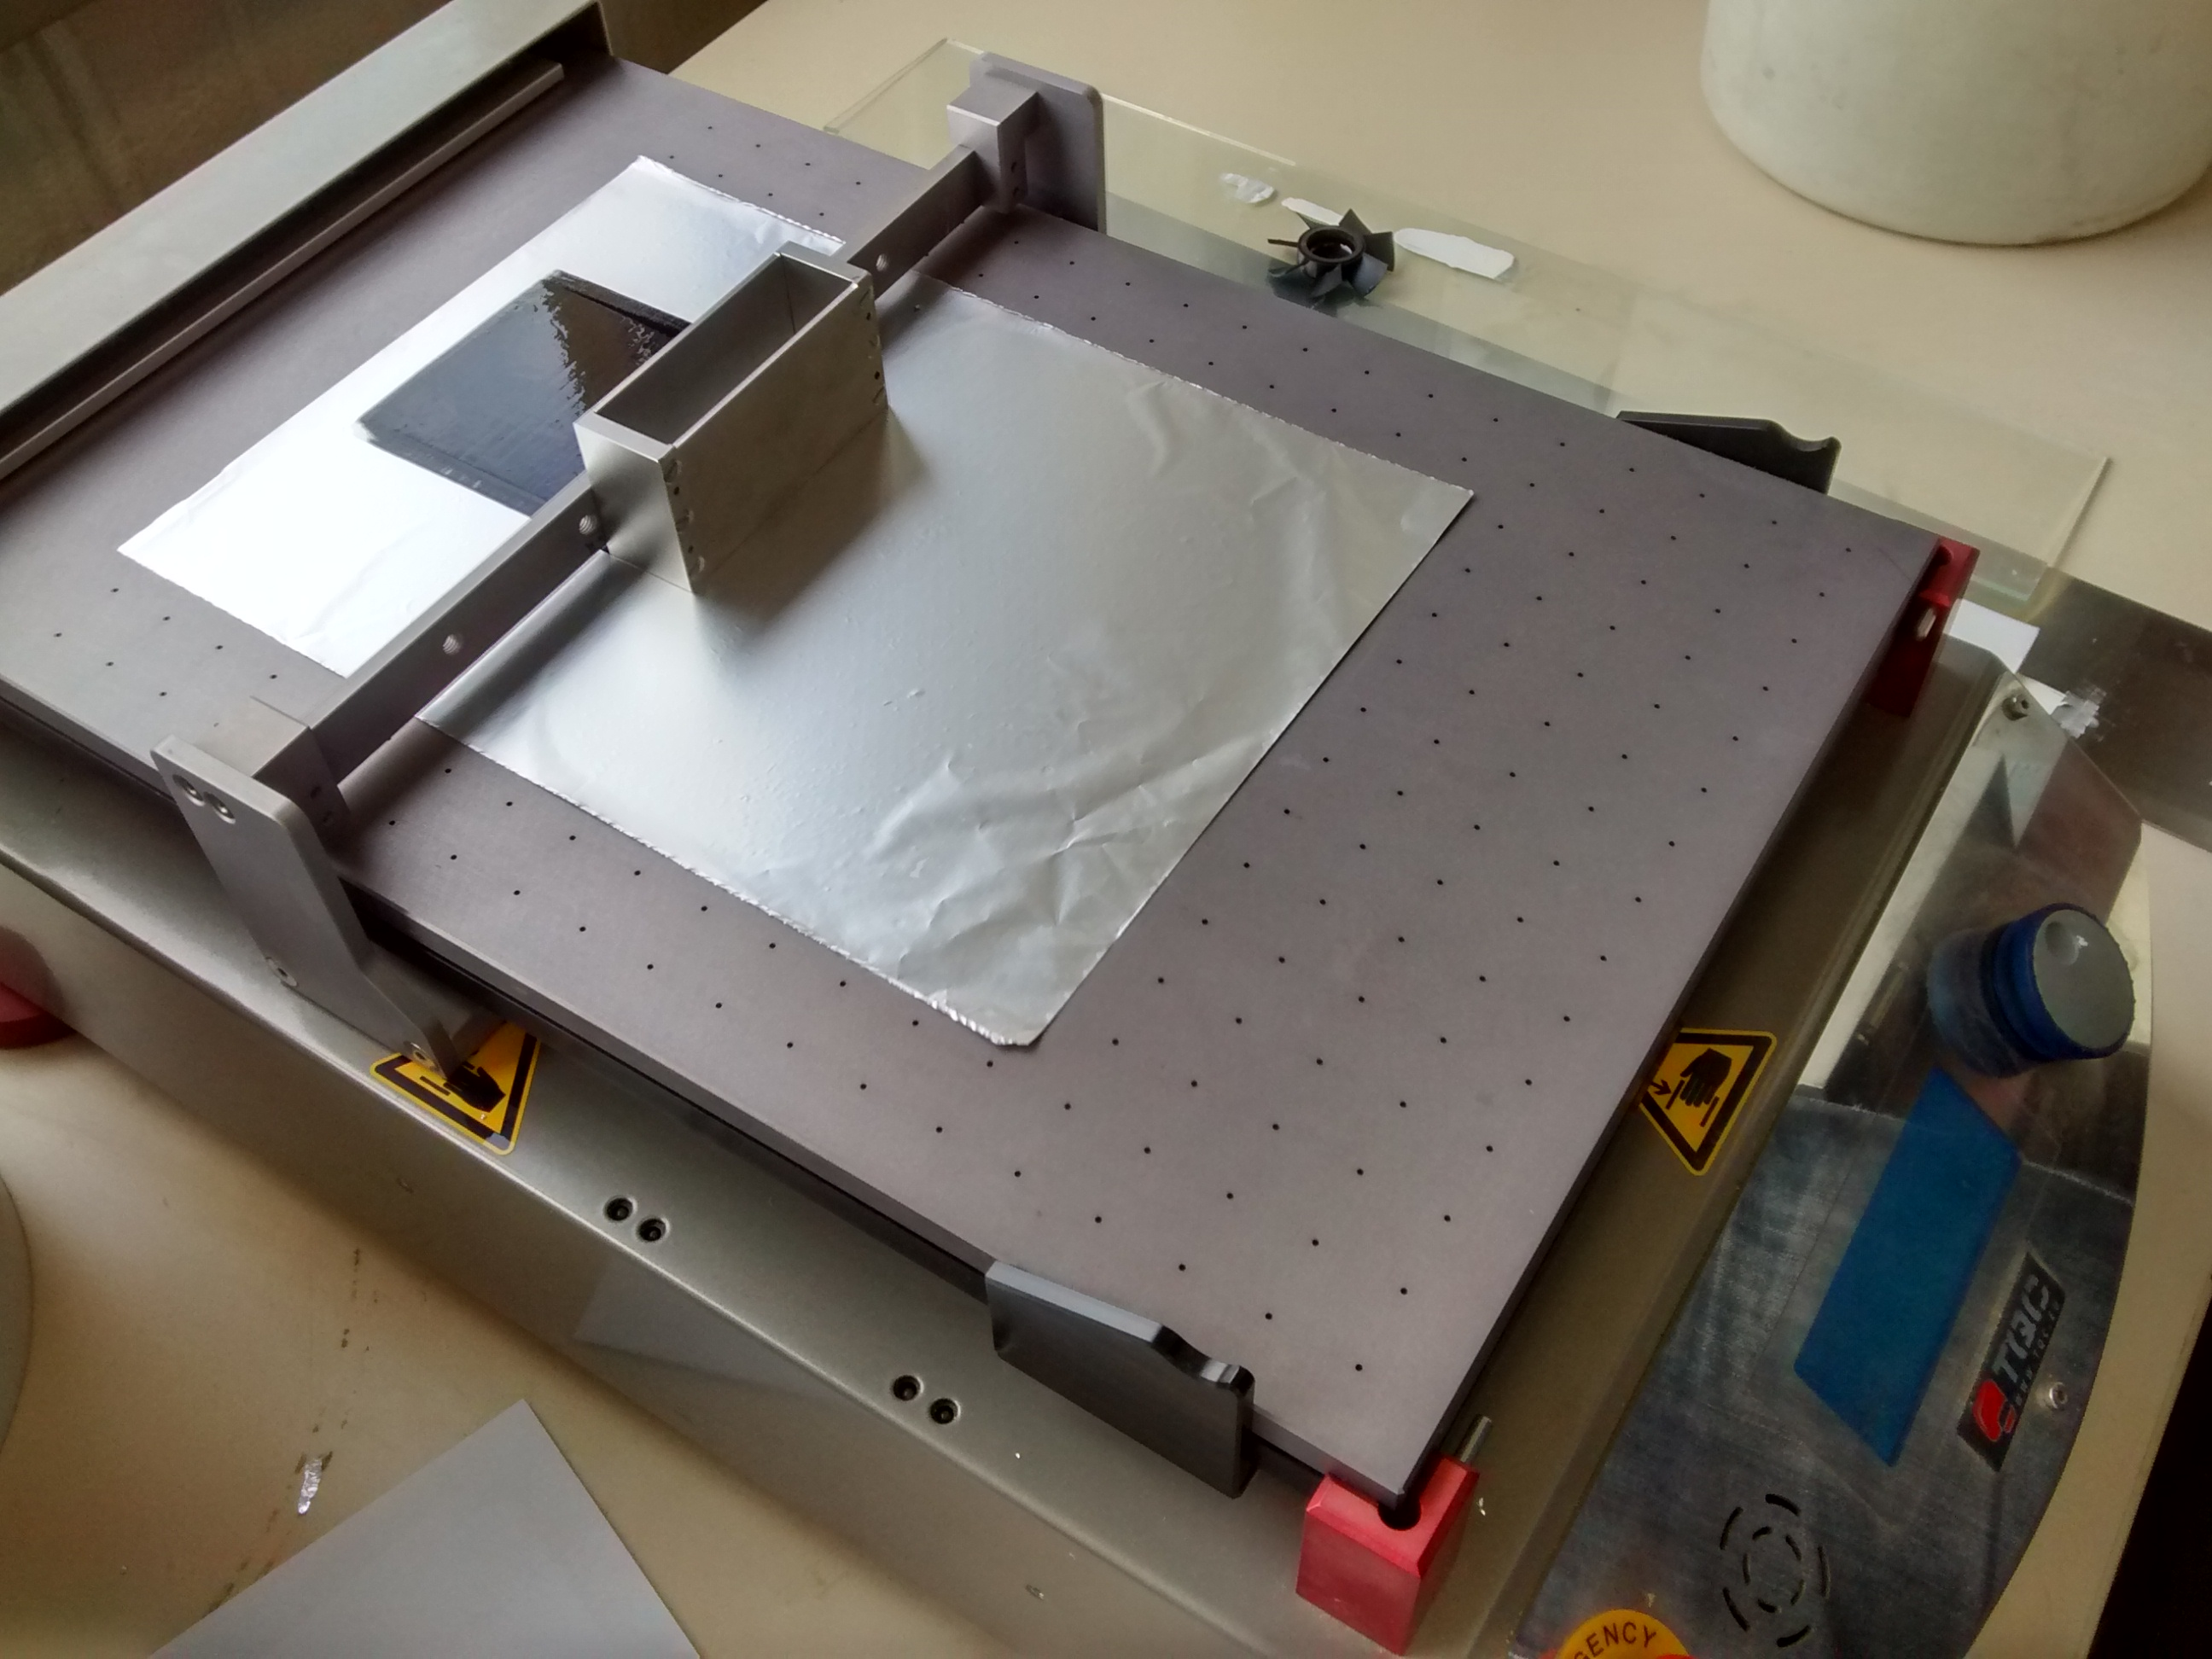
\includegraphics[width=0.82\columnwidth]{images/folienguss.jpg}
	\caption{Folienguss einer Elektrode auf Aluminiumfolie}
	\label{folienguss}
\end{figure}
\section{Sintern eines Elektrode-Elektrolyt-Gefüges}
Für die Herstellung eines Elektrode-Elektrolyt-Gefüges wird zunächst 1,2g LTO in eine Matrize für das Spark-Plasma-Sintern (SPS) mit einem Durchmesser von 20mm verteilt. Darauf werden 1,5g LLTO aufgebracht. Die Pulver werden mit einer Handpresse mit 3kN vorgepresst. Anschließend wird die Matrize in die SPS-Anlage eingebaut. 
\\\\
Die SPS-Anlage legt nach Einbau erstmal einen Druck von 5kN auf die Matrize auf. Der Druck wird dann auf 7,8kN erhöht, bevor die Temperatur mit 50$^\circ$C/min auf 900$^\circ$C angepasst wird. Diese Temperatur wird eine Minute gehalten, bevor der Druck für fünf Minuten auf 15kN gesteigert wird. Anschließend wird die Probe bei 7,8kN abgekühlt. 
%Eine Übersicht über den Prozess findet sich in Abbildung (noch einfügen).
\section{Bau und Betrieb der Batterie-Testzellen}
\label{bau_zellen}
\begin{figure}
	\centering
	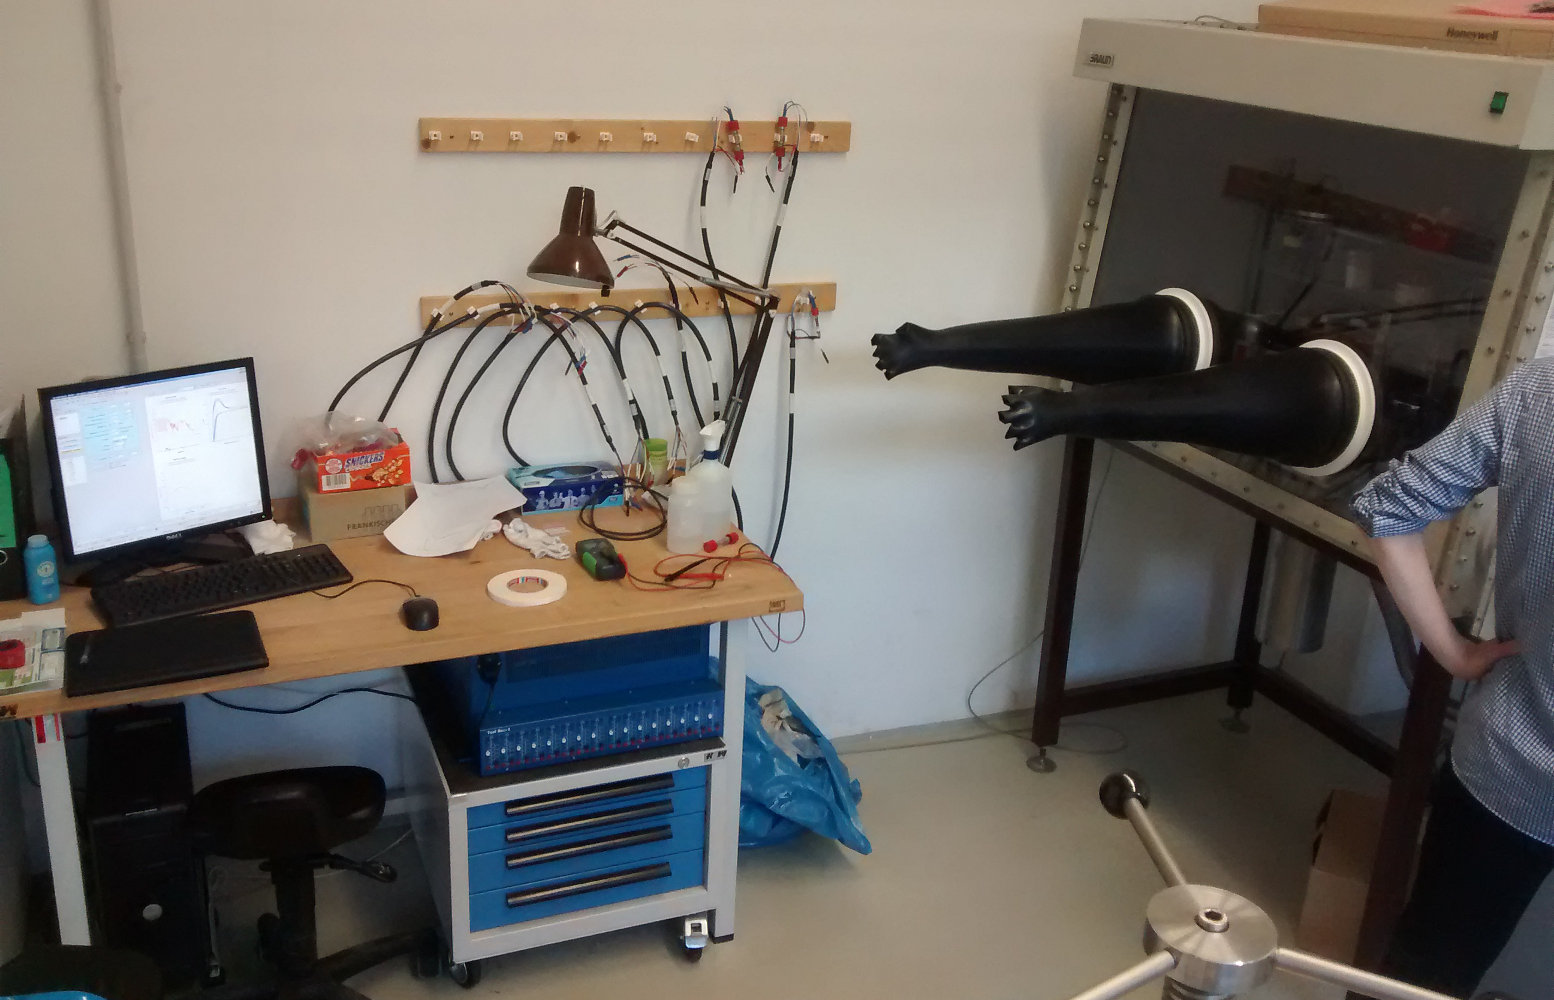
\includegraphics[width=0.95\columnwidth]{images/Messplatz.jpg}
	\caption{Messplatz für Batteriezellen mit Handschuhbox zum Bau (rechts), Ansteuerungselektronik und Aufbewahrung (mitte) sowie Kontrolle und Aufzeichnung durch Computer (links). --> Besseres Foto}
	\label{messaufbau}
\end{figure}
Zunächst werden aus den gegossenen Elektrodenfolien Proben entnommen. Dies geschieht händisch mit einem 10mm-Stanzeisen. Die Proben werden anschließend in eine Handschuhbox der Firma MBraun eingeschleust. Der Zusammenbau der Testzellen erfolgt dort unter Argonatmosphäre. Die Proben werden dabei jeweils als Kathode verbaut. Als Anode kommt Lithiummetall (99,9\%, Aldrich) zum Einsatz. Von diesem wird die äußerste Schicht abgetragen, um mögliche passivierte Stellen zu entfernen. Anschließend wird das Lithium mit einer Handwalze auf einen halben Millimeter gewalzt, wodurch seine Oberfläche geglättet wird. Danach kann mit einem 10mm-Stanzeisen die Lithium-Elektrode hergestellt werden.
\\\\
Der Zusammenbau besteht aus dem Einsetzen des unteren Stempels sowie eines Positionsplättchens in die Zelle. Darauf wird zunächst die Kathodenprobe gelegt und mit zwei Separatoren abgedeckt. Durch die zweifache Bedeckung führt ein Defekt eines Separators nicht zum Ausfall der Zelle. Die Separatoren werden mit 80$\mu$l Elektrolyt benetzt. Auf die Separatoren wird die Lithium-Anode und ein weiteres Positionsplättchen gelegt. Um einen Anpressdruck der Teile zu gewährleisten wird nun die Feder eingebaut und die Zelle mit dem oberen Stempel verschlossen. Beide Stempel können nun mit Mutter und Deckel fixiert werden. Danach kann die Zelle ausgeschleust und an das Messsystem angeschlossen werden.
% Was genau ist der Separator, was genau der Schwefel-Elektrolyt
\\\\
\subsection{Untersuchungsroutine der Batterietestzellen} %Evtl. in die Ergebnisse
Die Batteriezellen werden mit dem Messsystem VMP3 der Firma BioLogic untersucht. Dieses wird mit der Software ECLab in der Version 10.33 angesteuert und ermöglicht die Zyklierung der Zellen, zyklische Voltametrie sowie Impedanzmessungen. Die aufgezeichneten Daten können als zView-Datei exportiert und weiterverarbeitet werden.
% ECLab-Programme?

%%%%%%%%%%%%%%%%% 5. ERGEBNISSE %%%%%%%%%%%%%%%%%

\chapter{Ergebnisse}
Die angefertigten Pulver werden mittels Röntgendiffraktion untersucht. Für das LATP-, LAGP- und \ce{LiTiPO5}-Pulver werden außerdem noch Ergebnisse der Untersuchung mit der MAS-NMR-Spektroskopie vorgestellt.
\\\\
Für die hergestellten Batterieproben werden Ladekennlinien erstellt. Außerdem werden sie mittels zyklischer Voltametrie und Impedanzmessungen analysiert. Die Funktionalität der in-situ-Testzelle wird mit einer Lithium-Schwefel-Zelle gezeigt. Dazu erfolgt eine elektrochemische Voruntersuchung.
\section{Pulveranalyse}
Die Röntgenbeugungsexperimente wurden am Röntgendiffraktometer D500 der Firma Siemens durchgeführt. Dieses besitzt einen Bragg-Brentano-Aufbau. Abgefahren wurden in Gradschritten Winkel von 12 - 72$^\circ$. Die Verweilzeit in einer Stellung betrug fünf Sekunden. Die Analyse erfolgte durch Vergleich der erhaltenen Spektren mit einer Computerdatenbank.
\\\\
Die MAS-NMR-Spektroskopie wurde an einem Bruker-Spektroskopen mit einer H$^1$-Larmor\-frequenz von 400 MHz durchgeführt. Dies entspricht einer Stärke des äußeren Magnetfelds von 9,39 Tesla. Die Frequenz der Transmitterspule wurde deswegen für Li$^7$-Messungen auf 155,4 MHz eingestellt. Anschließend wurde der Nullpunkt der Messung mit einem Lithiumchlorid-Pulver (FIRMA) kalibriert. Der Spinner wurde mit vier unterschiedlichen Umdrehungsgeschwindigkeiten betrieben. Die Geschwindigkeit wurde dabei in 2 kHz-Schritten von 0 Hz auf 6kHz erhöht.
\newpage
\subsection{Pulvercharakterisierung des LATP}
\begin{figure}
   \centering
      \subfloat[Röntgendiffraktionsspektrum]{
	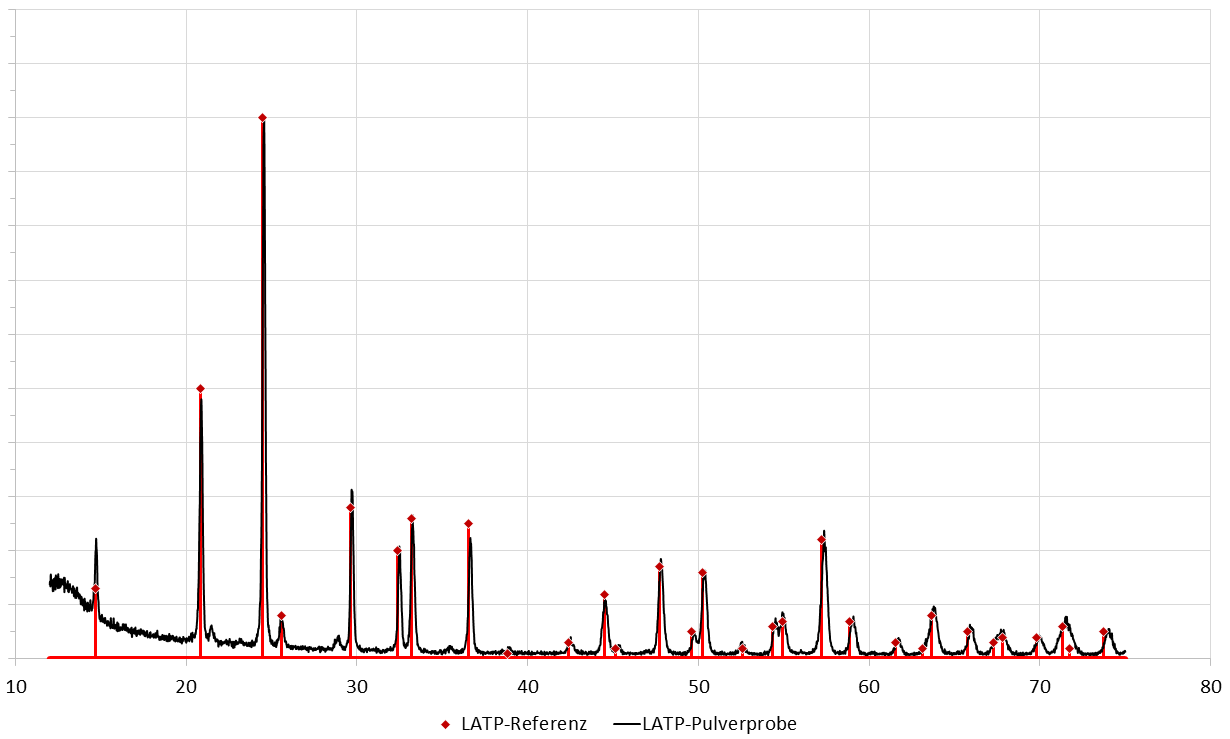
\includegraphics[width=1.0\columnwidth]{images/XRD_LATP.png}
	\label{xrd_LATP}
	} \vspace{6mm}
      \subfloat[MAS-NMR-Spektrum]{
	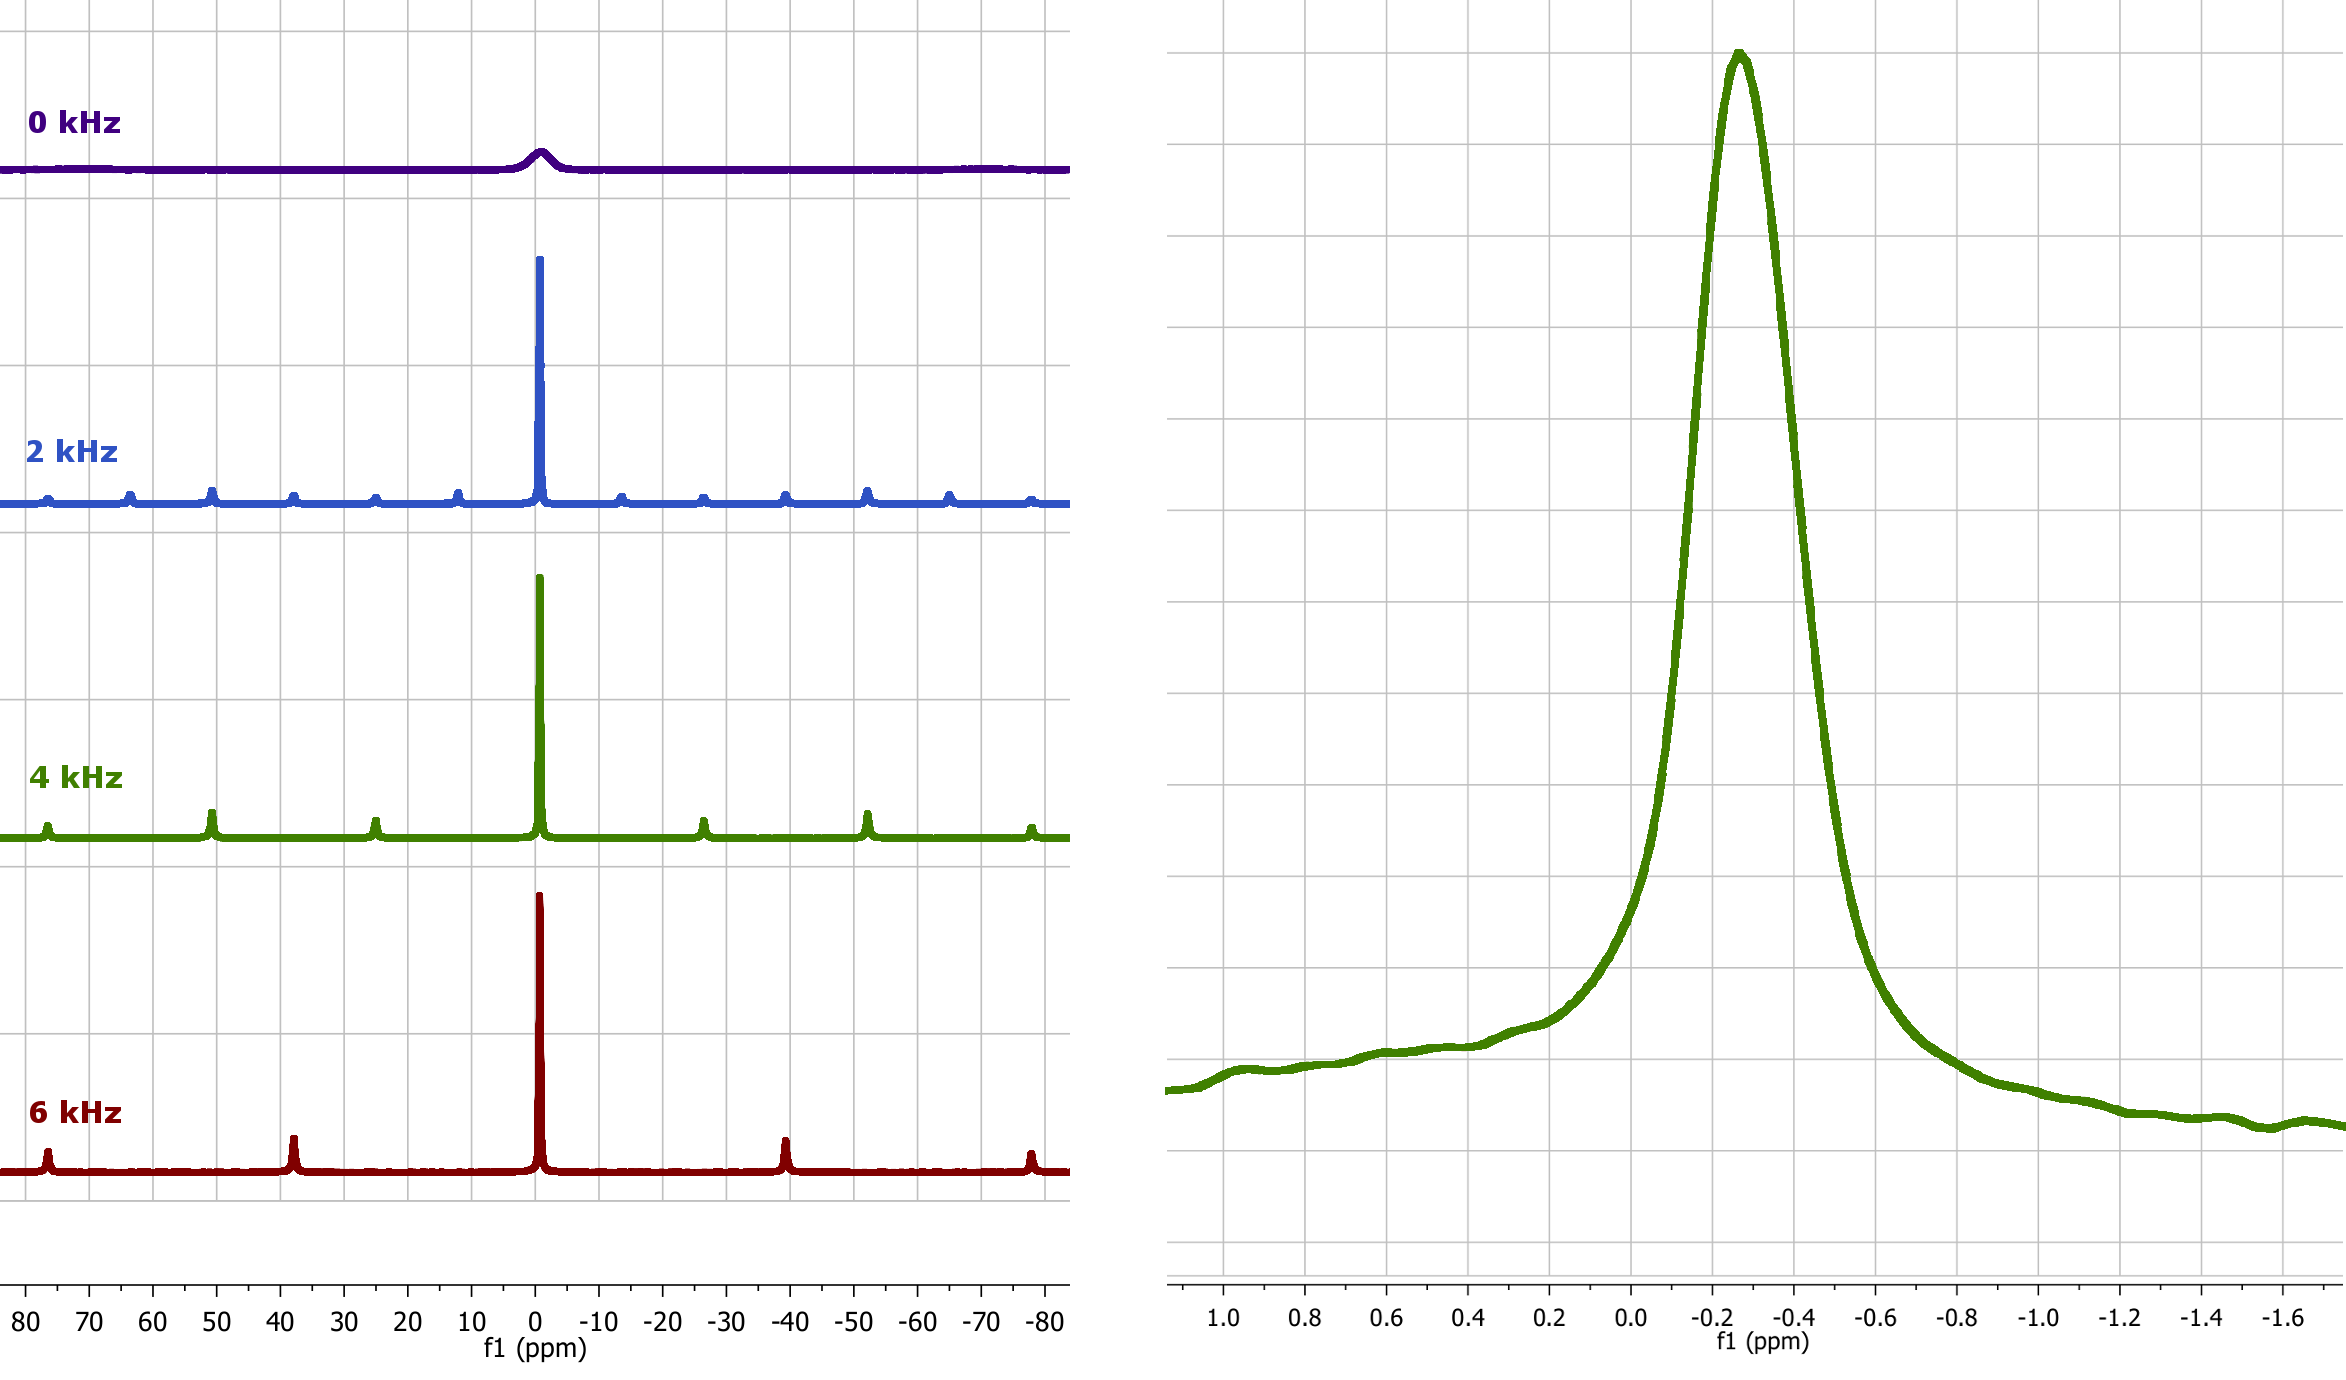
\includegraphics[width=1.0\columnwidth]{images/MAS_LATP.png}
	\label{mas_LATP}
      	} \vspace{3mm}
	\caption{Charakterisierung des LATP-Pulvers mit (a)~Röntgen\-diffraktionsspektrum und (b)~MAS-NMR-Spektrum (links Übersicht über verschiedene Umdrehungsgeschwindigkeiten, rechts Nahaufnahme des Hauptpeaks bei 4kHz)}
   	\label{pulver_LATP}
\end{figure}
Die Pulveranalyse erfolgte an einer LATP-Probe mit der in Kapitel \ref{praep_LATP} vorgestellten Sol-Gel-Routine.
\subsubsection{XRD-Analyse}
Die XRD-Analyse des LATP-Pulvers in Abbildung \ref{xrd_LATP} zeigt eine gute Übereinstimmung zwischen Referenz und Probe. Lediglich in den niedrigen Winkelberreichen kommt es zu einer leichten, systematischen Fehldetektierung. Es kann von einer hohe Phasenreinheit des eingesetzten Pulvers ausgegangen werden.
\subsubsection{MAS-NMR-Analyse}
Das MAS-NMR-Spektrum des LATP-Pulvers bei unterschiedlichen Umdrehungsgeschwindigkeiten wird in Abbildung \ref{mas_LATP} links dargestellt. Zu erkennen ist ein deutlicher Peak am geeichten Nullpunkt der Messung. Bei nicht vorhandener Umdrehung (0kHz) besitzt dieser noch eine sehr schwache Intensität und ist sehr breit. Bei den Messungen mit Rotation des Spinners ist ein deutlicher und intensiver Peak zu erkennen. Außerdem gibt es jeweils Seitenbänder, deren Abstand zum Hauptpeak proportional zur Umdrehungsgeschwindigkeit zunimmt.
\\\\
Der rechte Teil der Abbildung \ref{mas_LATP} zeigt eine höher aufgelöste Darstellung des Hauptpeaks. Es ist eine leichte Verschiebung des Peaks auf -0,3ppm zu erkennen. Der Peak ist nahezu symetrisch. 
\newpage
\begin{figure}
	\centering
	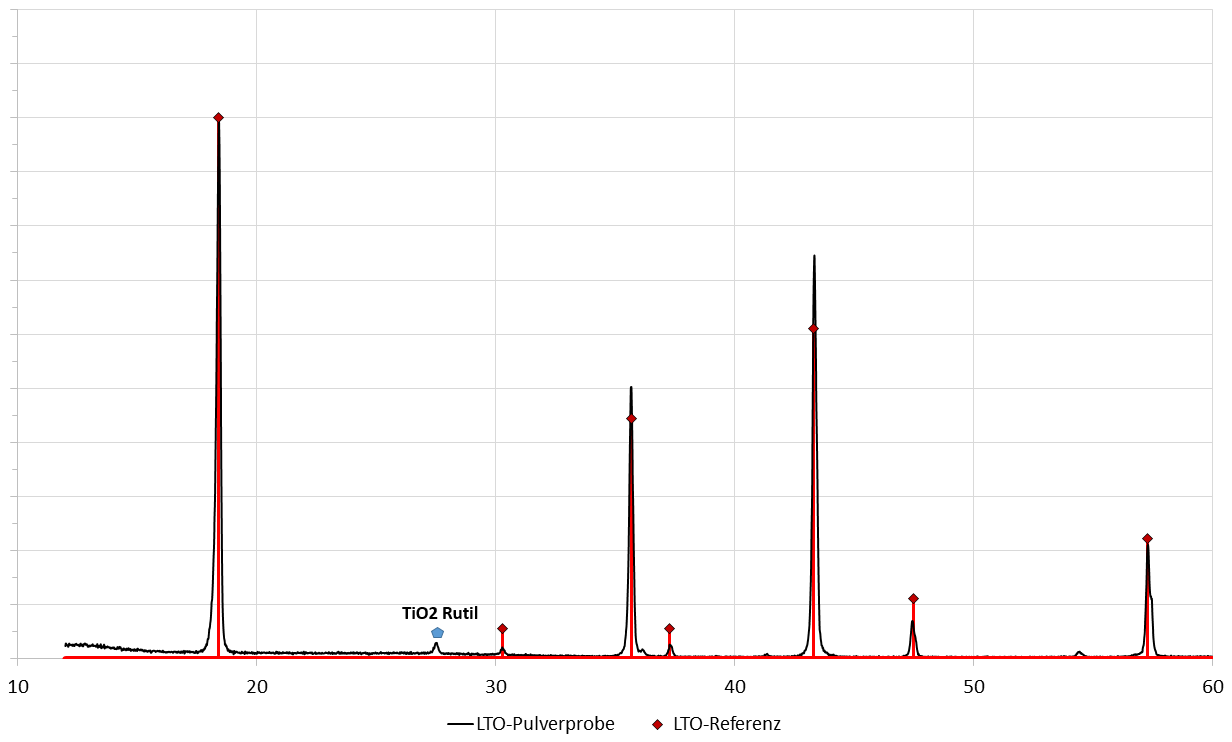
\includegraphics[width=1.0\columnwidth]{images/XRD_LTO.png}
	\caption{Röntgendiffraktionsspektrum der LTO-Probe}
	\label{xrd_LTO}
\end{figure}
\begin{figure}
   \centering
      \subfloat[Röntgendiffraktionsspektrum]{
	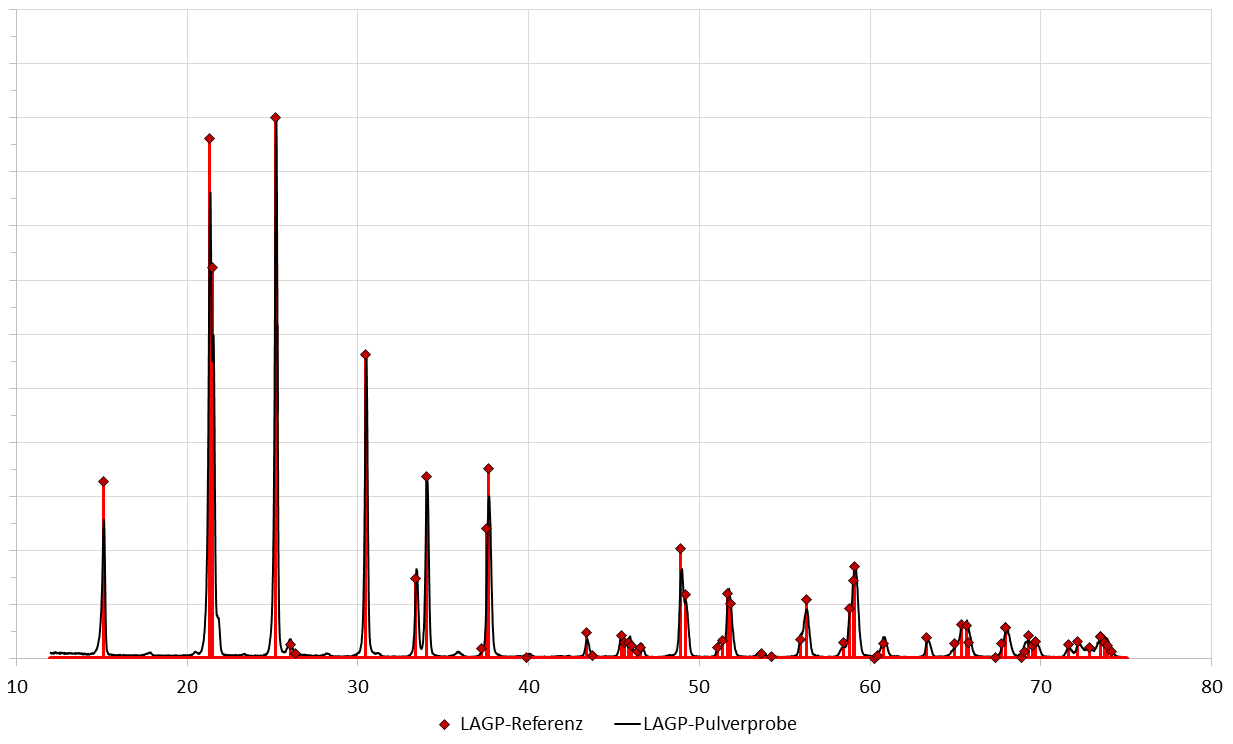
\includegraphics[width=1.0\columnwidth]{images/XRD_LAGP.png}
	\label{xrd_LAGP}
	} \vspace{6mm}
      \subfloat[MAS-NMR-Spektrum]{
	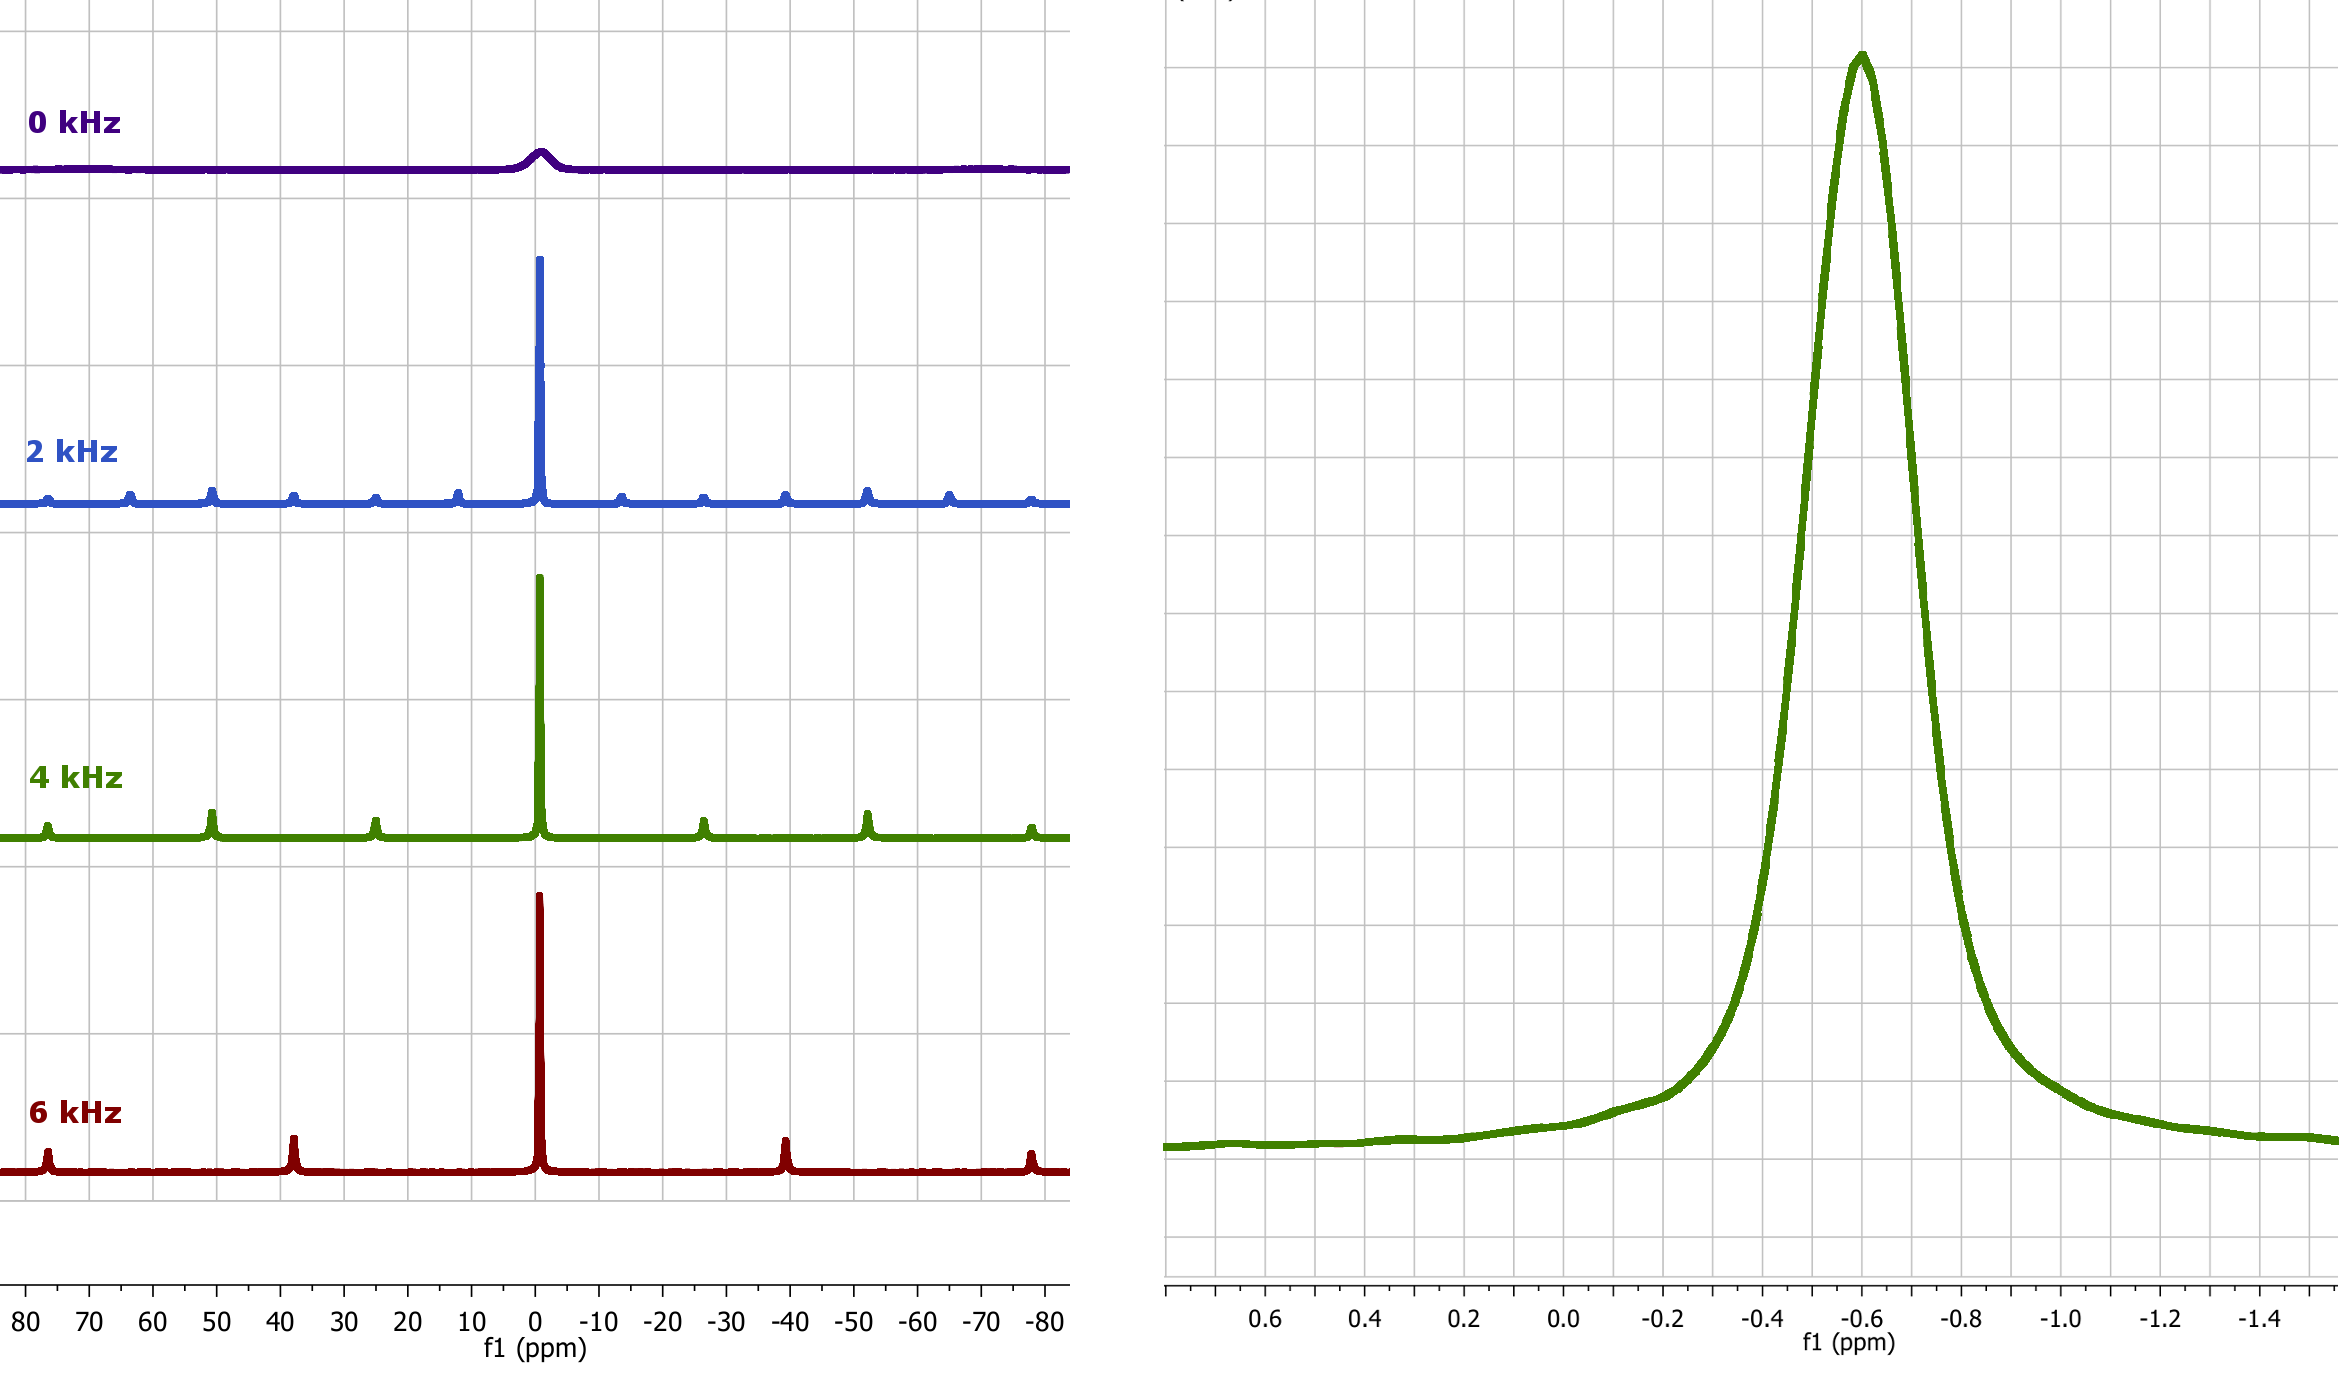
\includegraphics[width=1.0\columnwidth]{images/MAS_LAGP.png}
	\label{mas_LAGP}
      	} \vspace{3mm}
	\caption{Charakterisierung des LAGP-Pulvers mit (a)~Röntgen\-diffraktionsspektrum und (b)~MAS-NMR-Spektrum (links Übersicht über verschiedene Umdrehungsgeschwindigkeiten, rechts Nahaufnahme des Hauptpeaks bei 4kHz)}
   	\label{pulver_LAGP}
\end{figure}
\subsection{Pulvercharakterisierung des LTO}
Die Untersuchung der mit dem Mischoxid-Verfahren hergestellten LTO-Pulverprobe mittels XRD (Abbildung \ref{xrd_LTO}) ergibt eine gute Phasenreinheit des Pulvers. Bei \SI{27.5}{\degree} ist eine leichte Rutil (\ce{TiO2}) Fremdphase zu erkennen, die so allerdings auch im kommerziellen Produkt der Firma Sigma-Aldrich detektierbar ist. 
\subsection{Pulvercharakterisierung des LAGP}
Bei der LAGP-Probe erfolgte die Herstellung der Probe über den in Kapitel \ref{praep_LAGP} beschriebenen Sol-Gel-Prozess. 
\subsubsection{XRD}
Das Spektrum der röntgendiffraktometrische Untersuchung des LAGP-Pulvers in Abbildung \ref{xrd_LAGP} zeigt keine Zweitphasenanteile. Das verwendete Pulver ist daher phasenrein.
\subsubsection{MAS-NMR}
In Abbildung \ref{mas_LAGP} ist das MAS-NMR-Spektrum des LAGP-Pulvers zu sehen. Im linken Teil der Abbildung kann man dabei, äquivalent zu den bereits untersuchten Materialien, einen Hauptpeak bei etwa 0ppm mit von der Umdrehungsgeschwindigkeit abhängigen Seitenbändern erkennen. In der rechts abgebildeten Nahaufnahme des Peaks lässt sich dieser auf -0,6ppm bestimmen. Der Peak ist scharf und symetrisch.
\newpage
\begin{figure}
	\centering
	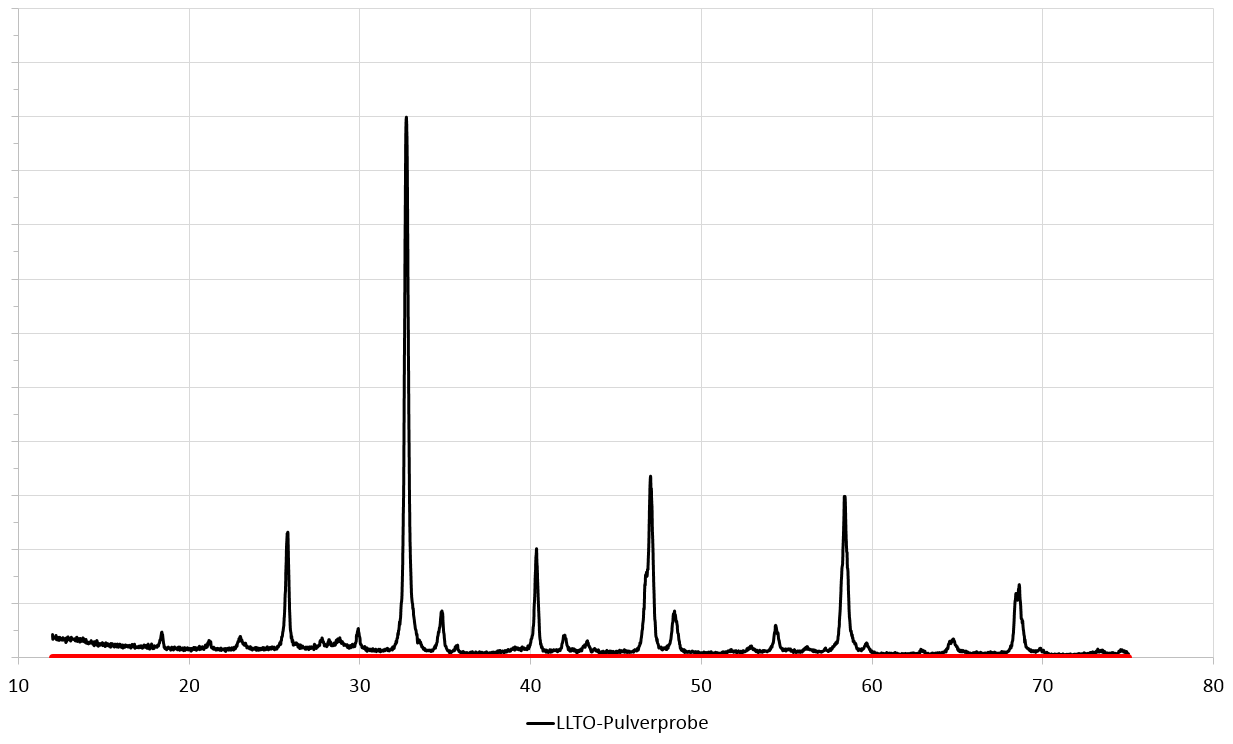
\includegraphics[width=1.0\columnwidth]{images/XRD_LLTO.png}
	\caption{Röntgendiffraktionsspektrum der LLTO-Probe}
	\label{xrd_LLTO}
\end{figure}
\begin{figure}
   \centering
      \subfloat[Röntgendiffraktionsspektrum]{
	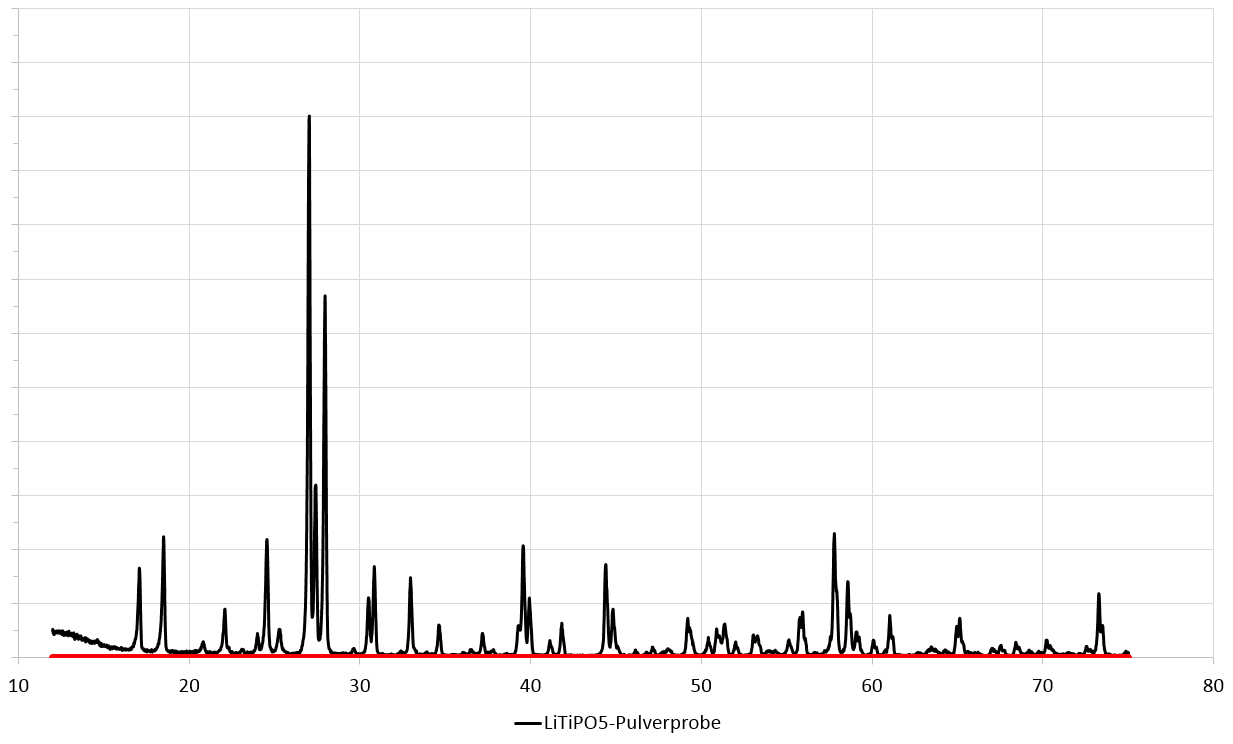
\includegraphics[width=1.0\columnwidth]{images/XRD_LiTiPO5.png}
	\label{xrd_LiTiPO5}
	} \vspace{6mm}
      \subfloat[MAS-NMR-Spektrum]{
	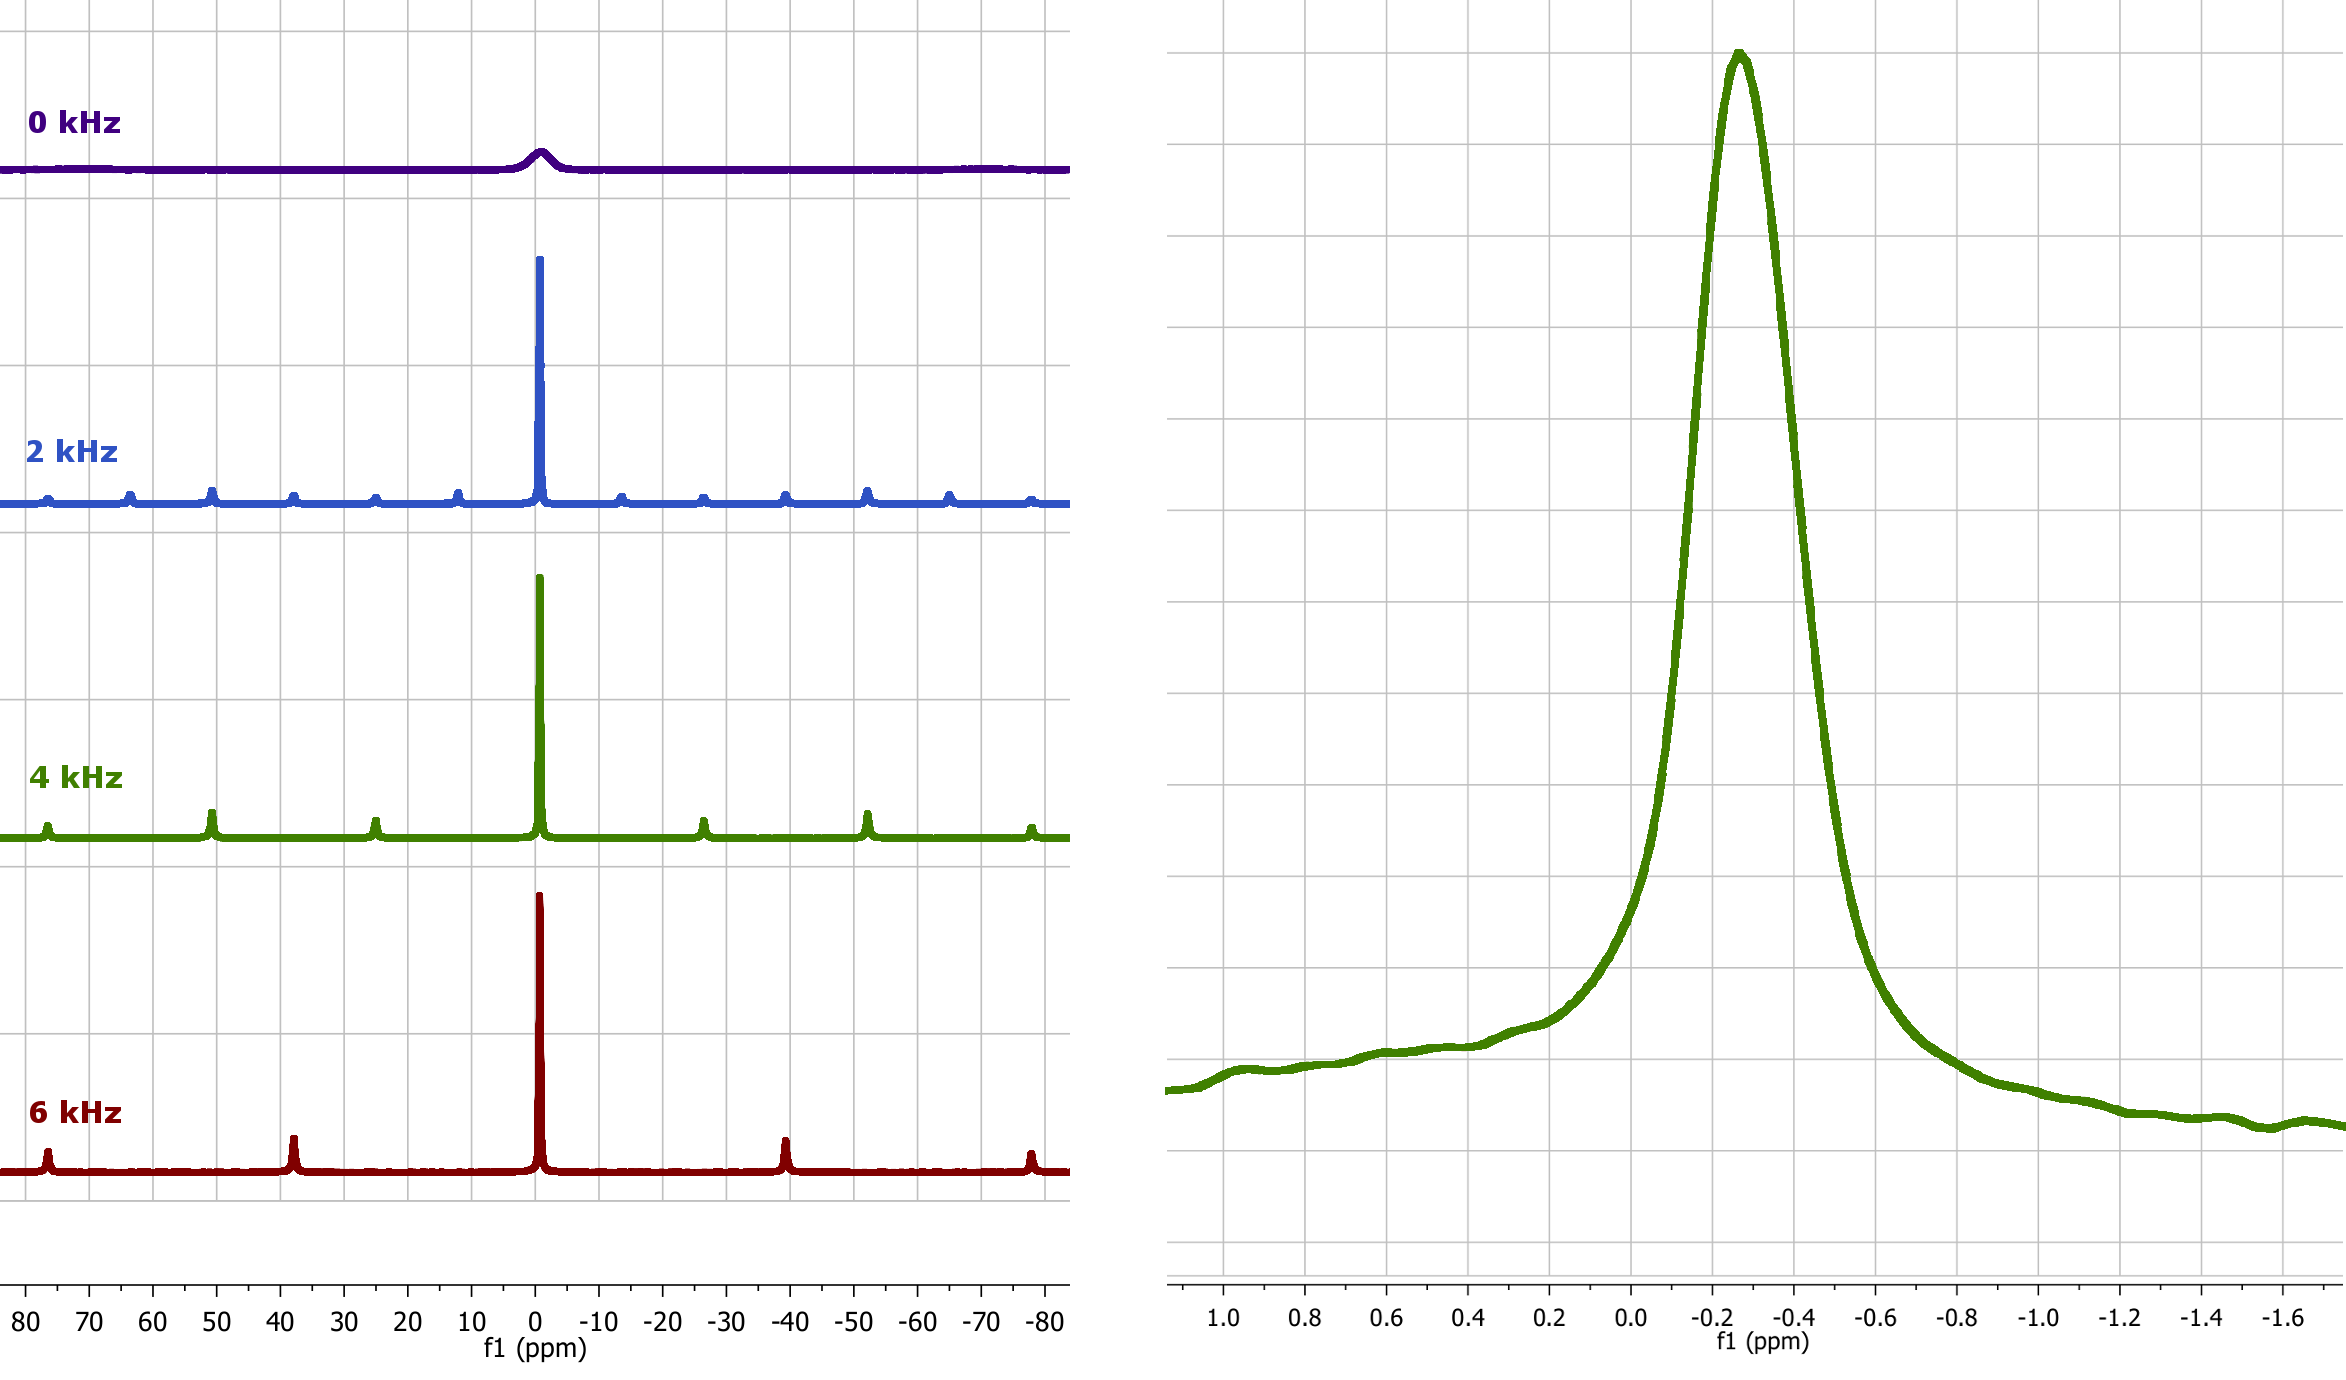
\includegraphics[width=1.0\columnwidth]{images/MAS_LATP.png}
	\label{mas_LiTiPO5}  
      	} \vspace{3mm}
	\caption{Charakterisierung des \ce{LiTiPO5}-Pulvers mit (a)~Röntgen\-diffraktionsspektrum und (b)~MAS-NMR-Spektrum (links Übersicht über verschiedene Umdrehungsgeschwindigkeiten, rechts Nahaufnahme des Hauptpeaks bei 4kHz)}
   	\label{pulver_LiTiPO5}
\end{figure}
\subsection{Pulvercharakterisierung des LLTO}
.
\subsection{Pulvercharakterisierung des \ce{LiTiPO5}}
Untersucht wird das im Sol-Gel-Prozess hergestellte \ce{LiTiPO5}. Die genaue Prozessierung über einen Sol-Gel-Prozess findet sich in Kapitel \ref{praep_LiTiPO5}.
\subsubsection{XRD-Analyse}
Im XRD-Spektrum, dargestellt in Abbildung \ref{xrd_LiTiPO5}, sieht man eine gute Übereinstimmung zwischen Referenz und gemessenen Werten. Es ist daher von einer hohen Phasenreinheit des untersuchten Pulvers auszugehen.
\subsubsection{MAS-NMR-Analyse}
.
\newpage
\section{Untersuchung der Elektrodenfolie mittels REM/EDX}
Die Beschaffenheit der gegossenen Elektrodenfolien wurde mit Aufnahmen des Rasterelektrodenmikroskops (REM) und an ausgewählten Stellen mittels einer energiedispersiven Röntgenspektroskopie (energy dispersive X-ray-spectorscopy, EDX) untersucht.
\subsubsection{REM}
Eine Übersicht  über die REM-Aufnahmen der unterschiedlichen Folien ist in Abbildung \ref{uebersicht_rem} dargestellt. Zu erkennen sind helle Partikel, welche das Aktivmaterial innerhalb der Probe sind. Die Aluminiumfolie ist als helle, massive  und klar abgetrennte Schicht sichtbar, während der Leitruß eine poröse, dunkle Struktur bildet. Das Aktivmaterial ist in allen Folien gut über die gesamte Höhe der Elektrode verteilt und liegt weder sedimentiert noch stark agglomeriert vor. Es ist jedoch eine gewisse Neigung zur Agglomeration zu erkennen, die vor allem bei der LAGP-Probe zu einigen größeren Agglomeraten führt. Bei der Struktur des Leitrußes lässt sich eine im Nanometerbereich fein verästelte und hochporöse Struktur ausmachen, in die sich das Aktivmaterial einbaut. Die Höhe der Elektrodenschicht lässt sich mit den Aufnahmen auf 40$\mu$m bestimmen, die der Aluminiumfolie auf 7,5$\mu$m.
\subsubsection{EDX}
Für eine genauere Materialuntersuchung wurden anschließend noch EDX-Aufnahmen angefertigt, die in Abbildung \ref{edx_gesamt} dargestellt werden. Mit diesen konnten die bisher gemachten Aussagen über die beteiligten Materialien bestätigt werden. Eine Verunreinigung der Suspensionen durch andere Partikel kann ebenfalls ausgeschlossen werden. Lediglich in der Aufnahme des LTO in \ref{edx_LTO} sind vereinzelt Aluminiumpartikel auf der Elektrodenfolie zu erkennen. Diese dürften ihren Ursprung im nicht perfekten Zuschnitt der Folie haben.
\begin{figure}
	\centering
	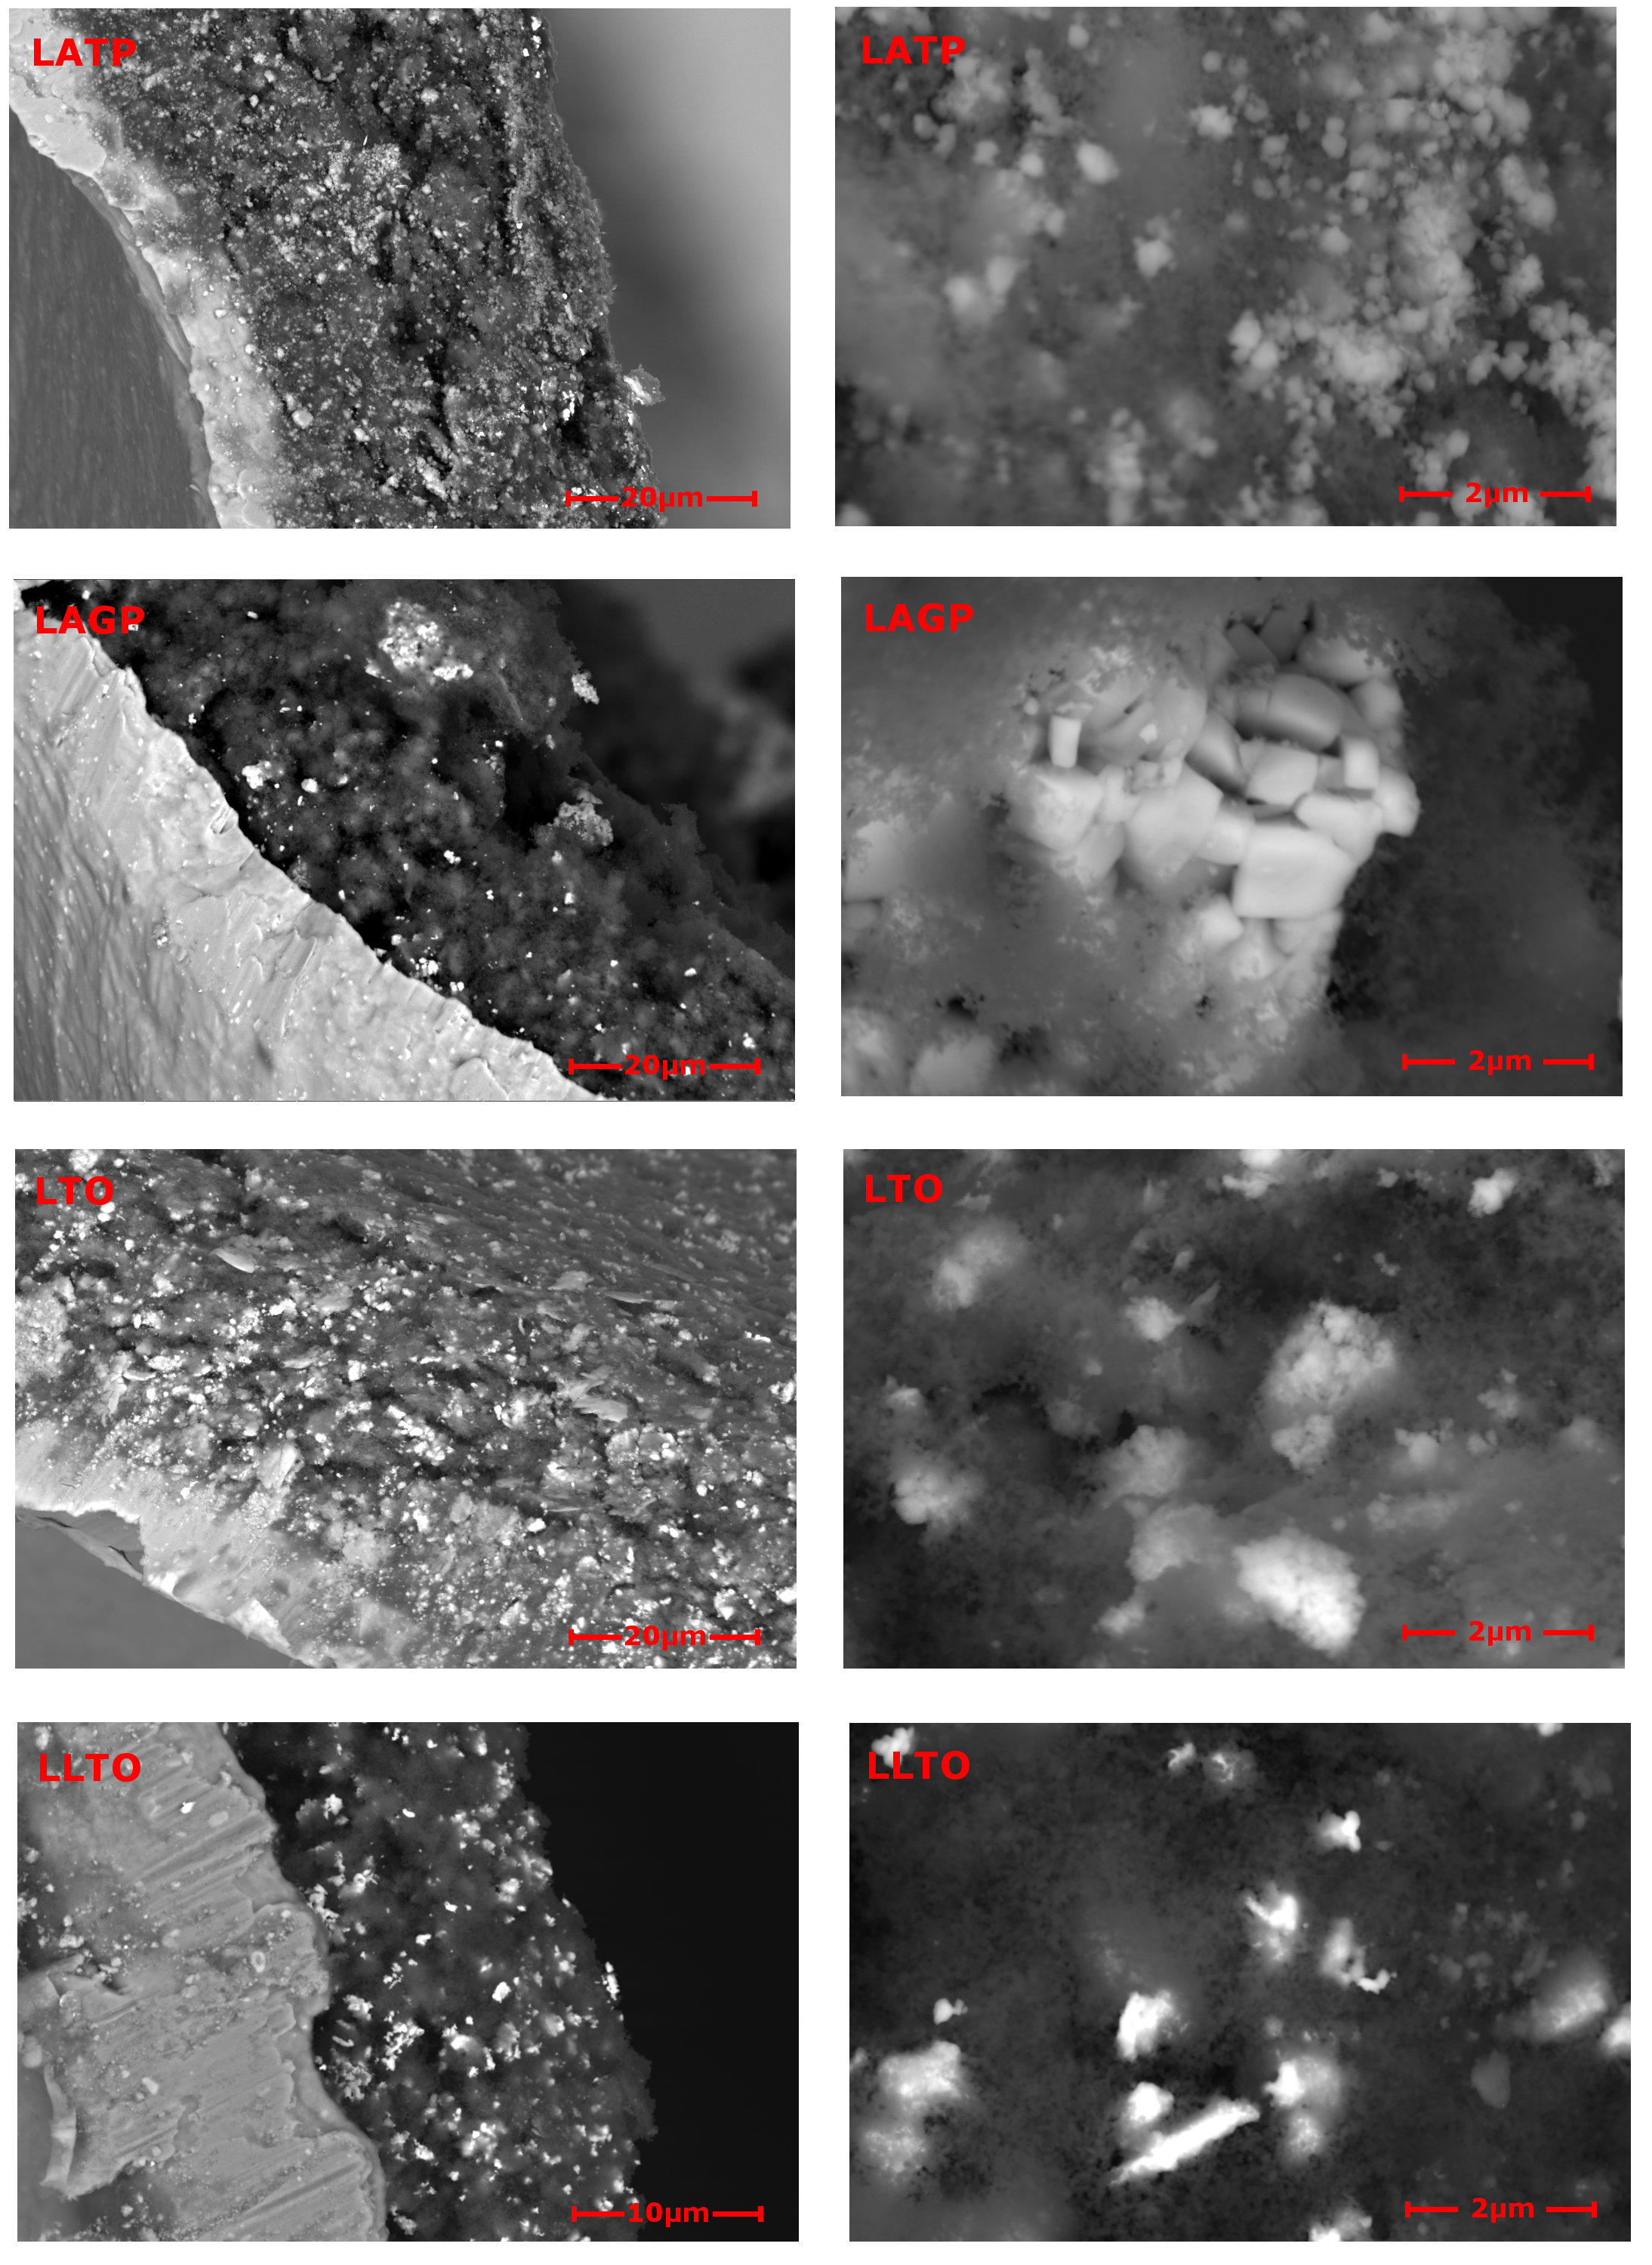
\includegraphics[width=1.0\columnwidth]{images/Uebersicht_REM.jpg}
	\caption{REM-Aufnahmen der verschiedenen Elektrodenfolien bei unterschiedlichen Vergrößerungsgraden}
	\label{uebersicht_rem}
\end{figure}
\begin{figure}
   \centering
      \subfloat[LATP]{
	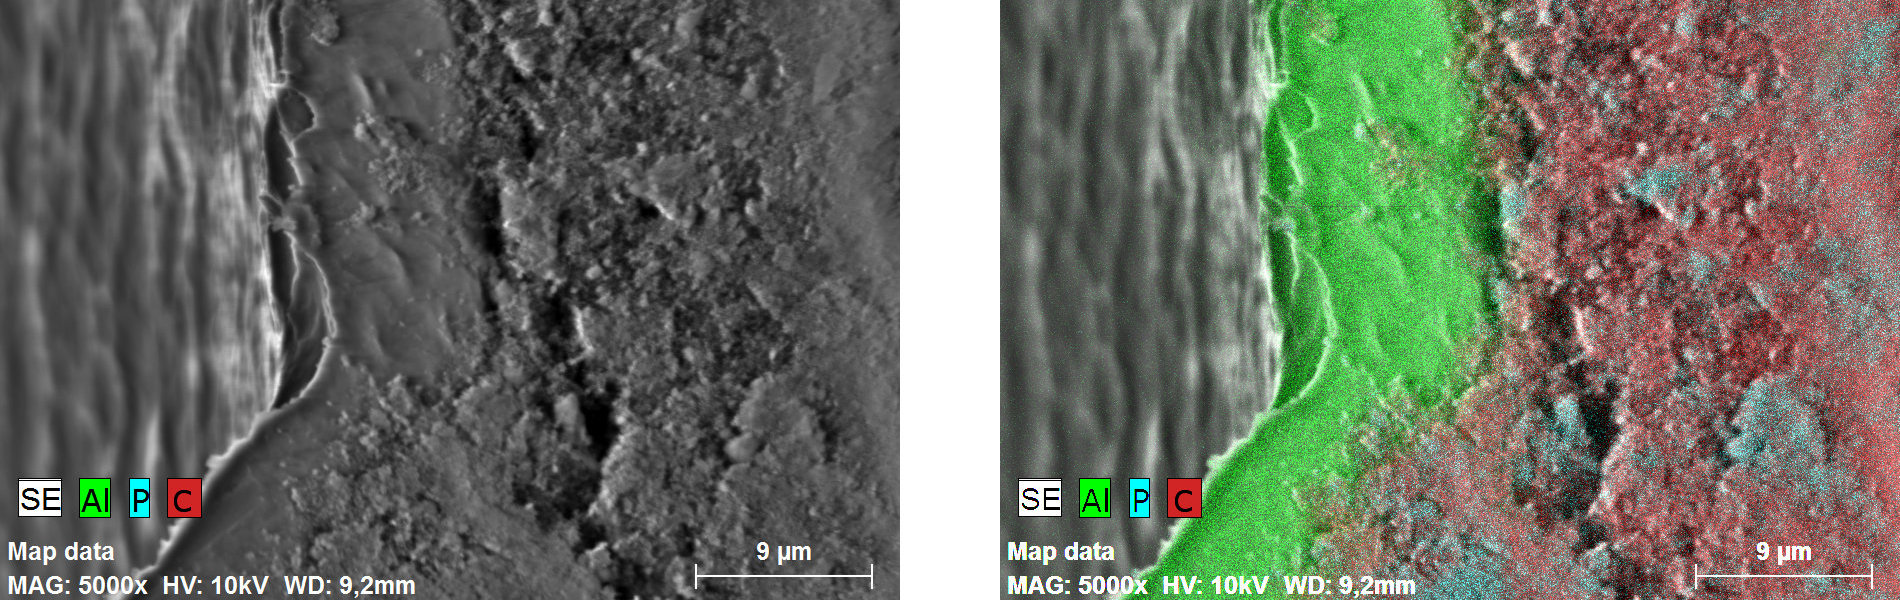
\includegraphics[width=1.0\columnwidth]{images/EDX_LATP.jpg}
	\label{edx_LATP}
	} \vspace{3mm}
      \subfloat[LAGP]{
	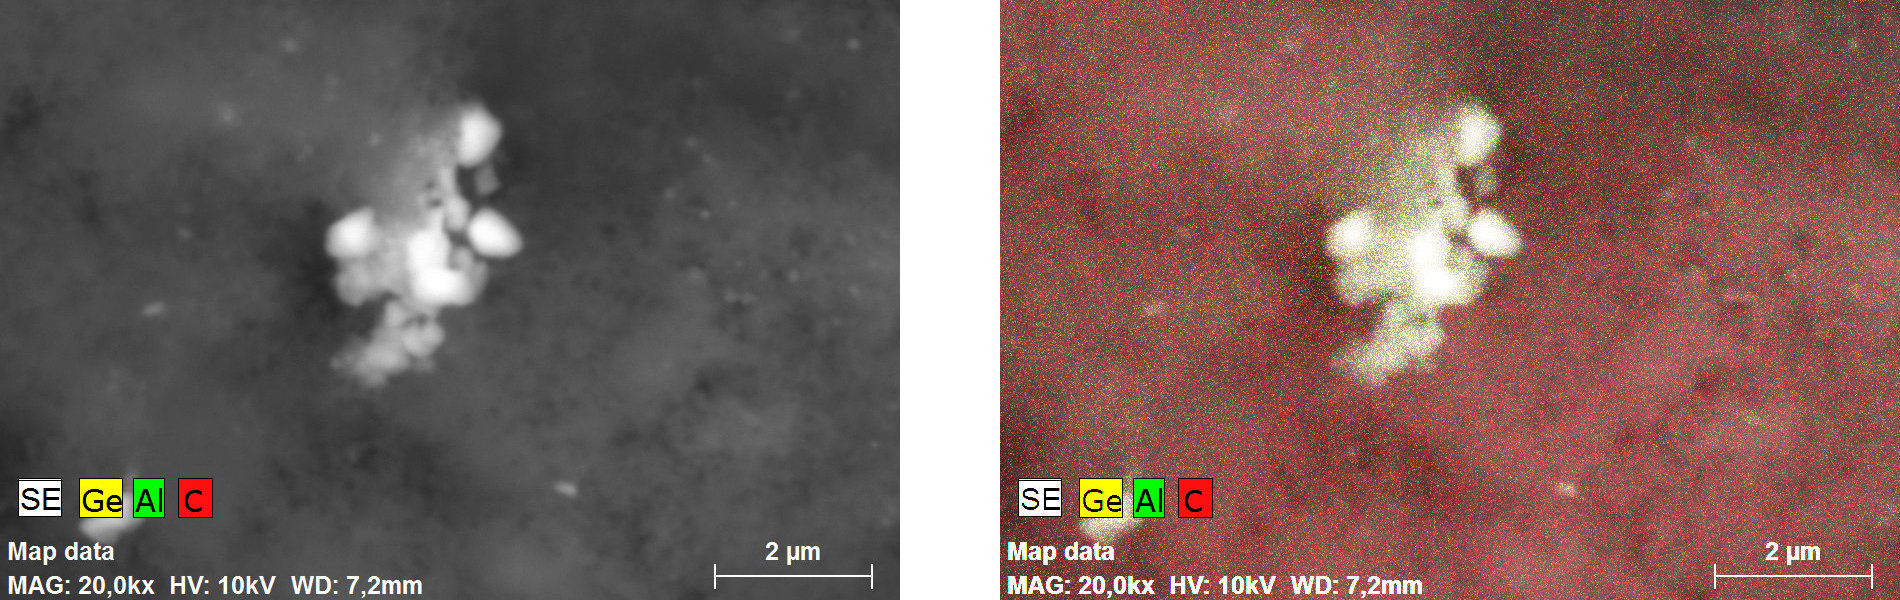
\includegraphics[width=1.0\columnwidth]{images/EDX_LAGP.jpg}
	\label{edx_LAGP}   
      	} \vspace{3mm}
      \subfloat[LTO]{
	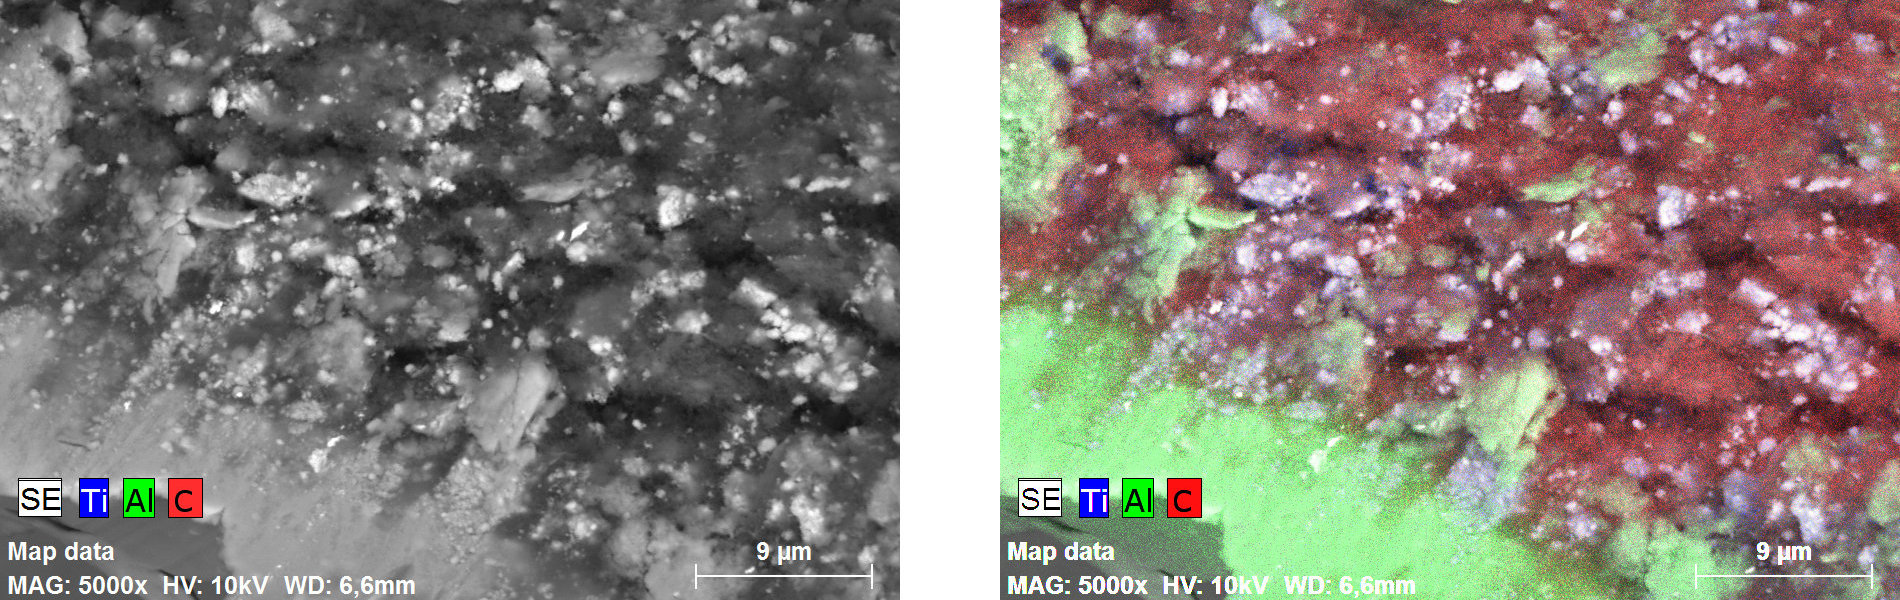
\includegraphics[width=1.0\columnwidth]{images/EDX_LTO.jpg}
	\label{edx_LTO}
	} \vspace{3mm}
      \subfloat[LLTO]{
	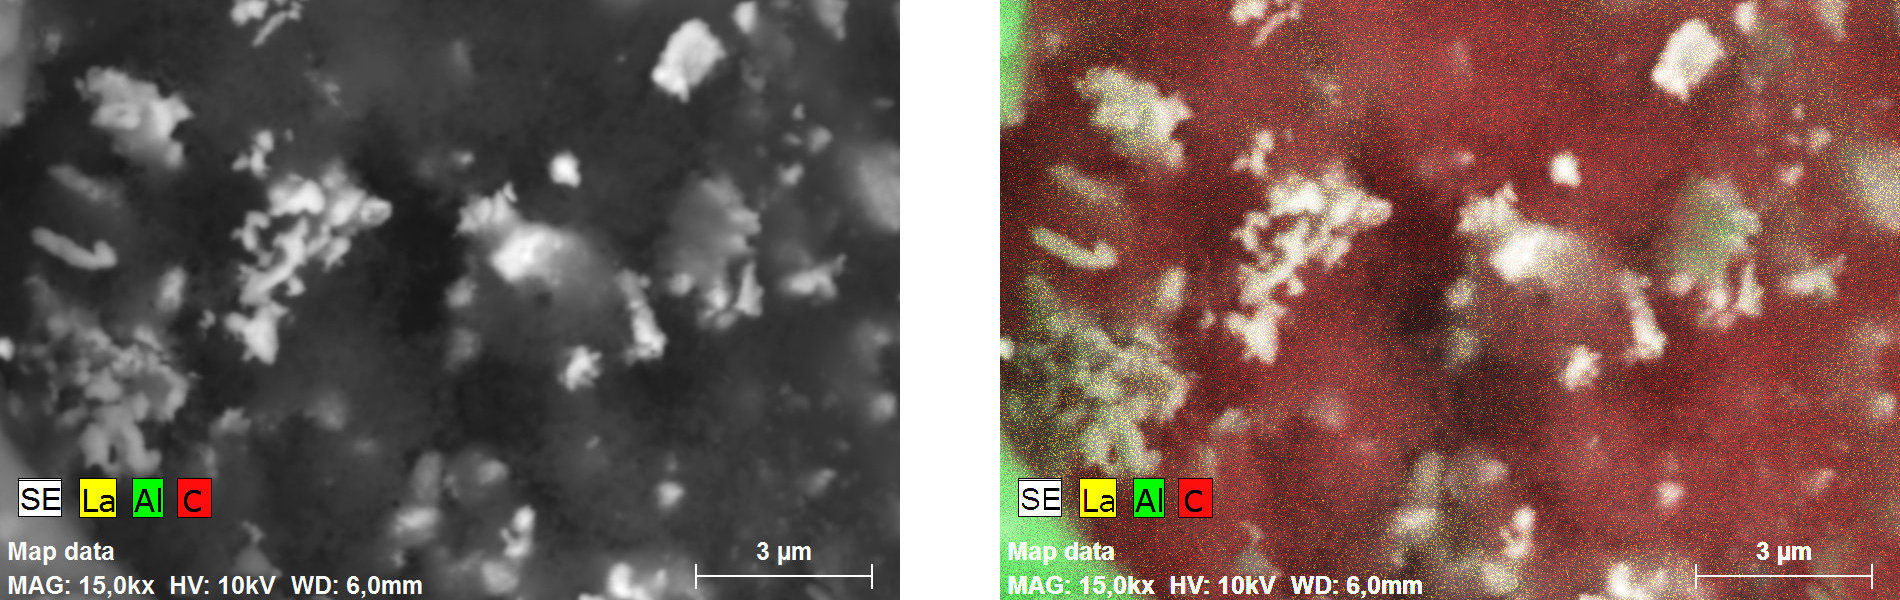
\includegraphics[width=1.0\columnwidth]{images/EDX_LLTO.jpg}
	\label{edx_LLTO}  
      	} \vspace{3mm}
	\caption{EDX-Aufnahmen der unterschiedlichen Folienproben}
   	\label{edx_gesamt}
\end{figure}
\newpage
\section{Bestimmung der Masse des Aktivmaterial}
Um das Gewicht des Aktivmaterials einer gestanzten Elektrodenprobe zu bestimmen, wurden jeweils fünf Proben aus der gegossenen und getrockneten Elektrodenfolie sowie auch aus der unbehandelten Aluminiumfolie gestanzt. Diese Proben wurden anschließend abgewogen und das resultierende Gewicht gemittelt. Die Masse der unbehandelten Aluminiumfolie wurde so zu 2,93mg bestimmt. Aus der Differenz aus Gesamtmasse und dem Gewicht der Aluminiumfolie konnte dann die Masse des Elektrodenmaterials der Probe bestimmt werden.
\\\\
Da der Massenanteil des jeweiligen Aktivmaterials auf 45\% der gesamten Elektrode eingewogen worden ist, kann dann die Masse des Aktivmaterials an einer Elektrodenprobe mittel Multiplikation mit diesem Faktor berechnet werden. Eine Übersicht über die so für alle Elektrodenproben bestimmten Massen findet sich in Tabelle \ref{tabelle_massen}.
\\
\begin{table}[h]
\begin{tabular}{L{1.2cm} L{4.6cm} L{1.8cm} L{1.8cm} L{1.8cm} L{1.8cm}}
\toprule
 & & \textbf{LATP} & \textbf{LAGP} & \textbf{LLTO}& \textbf{LTO}\\
\midrule
\multirowbt{3}{*}{\textbf{Masse}} & \textit{Elektrode mit Kollektor} &  \SI{4.71}{\milli\gram} &   \SI{3.98}{\milli\gram}  &  \SI{4.05}{\milli\gram}& \SI{4.28}{\milli\gram}\\
\cmidrule{2-6}
 & \textit{Elektrode ohne Kollektor} &   \SI{1.78}{\milli\gram} &  \SI{1.05}{\milli\gram} &  \SI{1.12}{\milli\meter}& \SI{1.35}{\milli\gram}\\
\cmidrule{2-6}
 & \textit{Aktivmaterial} &   \SI{0.80}{\milli\gram} &   \SI{0.47}{\milli\gram} & \SI{0.50}{\milli\gram}& \SI{0.61}{\milli\gram}\\
\bottomrule
\end{tabular}
 \caption{Massen der unterschiedlichen Proben.}
 \label{tabelle_massen}
 \end{table} 
\section{Elektrochemische Analyse der Elektrodenproben}
\label{elektrochemische_analyse}
Alle Elektrodenproben wurden als Kathoden gegen reines Lithiummetall verbaut und insgesamt elf mal ge- und entladen. Dabei wurde jeweils ein Lade- und Entladestrom von 50$\mu$A angelegt, bis eine definierte Abbruchspannung erreicht wurde.
\\\\
Bei der zyklischen Voltametrie wurden die Grenzen der Messung jeweils so gewählt, dass möglichst alle Reaktionen innerhalb der Zelle abgebildet wurden. Problematisch dabei war der Einfluss des Graphits innerhalb des Leitrußes. Dieser ist in der Lage Lithiumionen interkalieren zu lassen. Diese Reaktion findet bei einem abnehmenden Potential von etwa 0,6V statt, beginnt jedoch schon im Bereich zwischen 1,0 und 1,2V. Um eine vom Graphiteinfluss möglichst freie Messung aufnehmen zu können, wurde daher der untere Zyklierbereich so gewählt, dass gerade der beginnende Graphitpeak zu erkennen ist.
\\\\ % WERTE CHECKEN!
Die Impedanzmessungen fanden jeweils in einem Frequenzbereich von 1 Hz bis 1 MHz statt. Die dabei angelegte Spannung der Sinusamplitude betrug 10mV. Es wurden sechs Messpunkte pro Zehnerpotenz aufgenommen. % Messpunkte, Zeit 
\newpage
\subsection{LATP-Kathode}
\begin{figure}
   \centering
      \subfloat[Ladekennlinie]{
	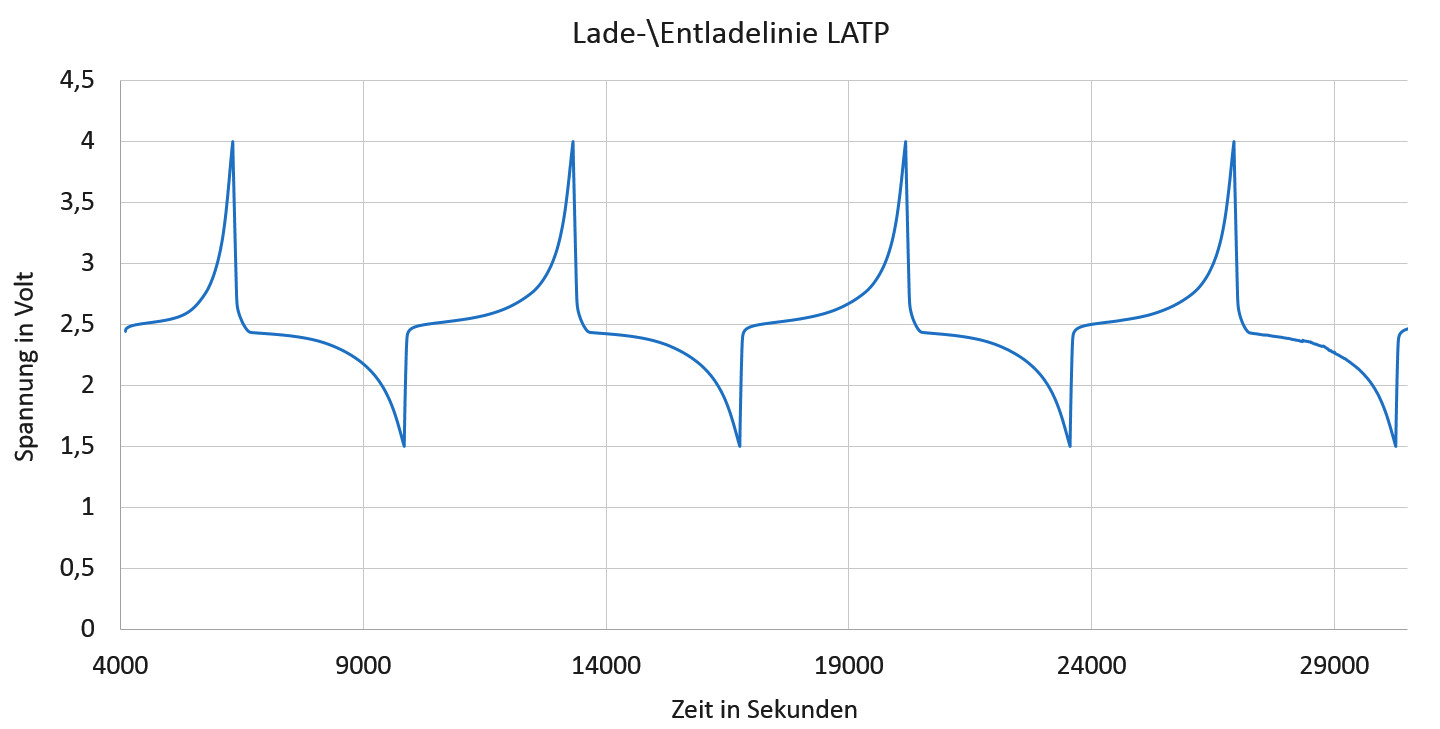
\includegraphics[width=1.00\columnwidth]{images/GCPL_LATP.jpg}
	\label{gcpl_LATP}
	} \vspace{3mm}
      \subfloat[Zyklische Voltametrie]{
	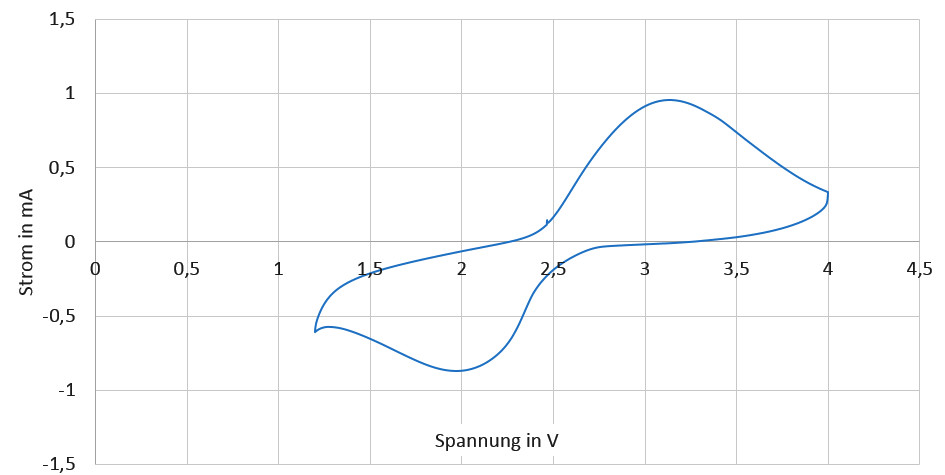
\includegraphics[width=0.85\columnwidth]{images/CV_LATP.jpg}
	\label{cv_LATP}   
      	} \vspace{3mm}
      \subfloat[Impedanzspektroskopie]{
	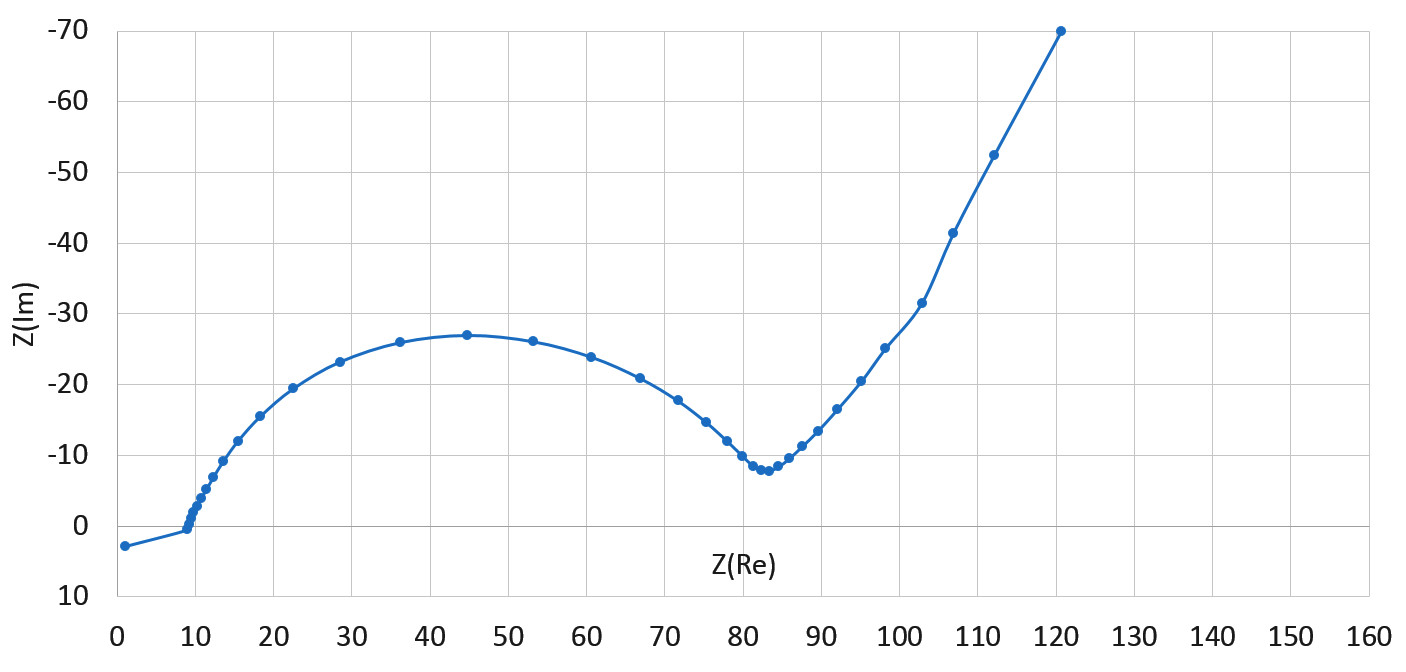
\includegraphics[width=0.85\columnwidth]{images/IS_LATP.jpg}
	\label{is_LATP}    
      	} \vspace{3mm}
	\caption{Charakterisierung des LATP mit (a)~Ladekennlinie, (b)~Zyklischer Voltametrie, (c)~Impedanzspektroskopie}
   	\label{ec_LATP}
\end{figure}
Die LATP-Probe wurde in einem Spannungsbereich von 1,5V bis 4,0V zykliert. Für die zyklische Voltametrie wurde der Potentialbereich von 1,2V bis 4,0V gewählt.
\subsubsection{Ladekennlinien}
Das LATP besitzt beim Laden der Zelle ein Plateau bei 2,55V. Schon nach kurzer Zeit geht die Zelle jedoch zu einem exponentiellem Anstieg der Spannung über, welche nach 59 Minuten die Abbruchspannung von 4V erreicht. Beim Anlegen des Entladestroms pendelt sich die Zelle auf eine Spannung von 2,45V ein. Äquivalent zum Laden kommt es beim Entladen schon nach kurzer Zeit zu einem exponentiell stärker werdenden Verfall der Entladespannung. Diese erreicht die Abbruchspannung ebenfalls nach 59 Minuten. Die zugehörige Kennlinie ist in Abbildung \ref{gcpl_LATP} dargestellt. 
\\\\
Die beim Entladen abgegebene elektrische Ladung sind 49$\mu$Ah. Die erreichte Kapazität der Probe lag bei einer Masse des Aktivmaterials von 0,80mg damit bei 61,3mAh/g. 
%Die C-Rate der Zyklierung liegt bei 0,57C.
\subsubsection{Zyklische Voltametrie}
Das Ergebnis der Untersuchung der Zelle mittels zyklischer Voltametrie ist in Abbildung \ref{cv_LATP} zu sehen. Es ergeben sich zwei Peaks. Der Peak im ansteigenden Potentialbereich liegt dabei bei 3,1V, der im absteigenden Bereich bei knapp über 2V. Beide Peaks sind mit über einem Volt sehr breit und führen nicht zur Nulllinie der Stromstärke zurück. Die Peaks sind nicht symetrisch, sondern nach außen hin breiter.
\subsubsection{Impedanzmessungen}
Die Messung der Impedanz wird in Abbildung \ref{is_LATP} im Nyquist-Plot dargestellt. Die Messung beschreibt einen Halbkreis, der bei einem Realteil von \SI{82}{\ohm} in eine im 45$^\circ$-Winkel ansteigende Gerade übergeht. Im hohen Frequenzbereich trifft der Graph bei einem Realteil von \SI{10}{\ohm} die X-Achse in einem Innenwinkel von etwa 75$^\circ$.
\newpage
\subsection{LAGP-Kathode}
\begin{figure}
   \centering
      \subfloat[Ladekennlinie]{
	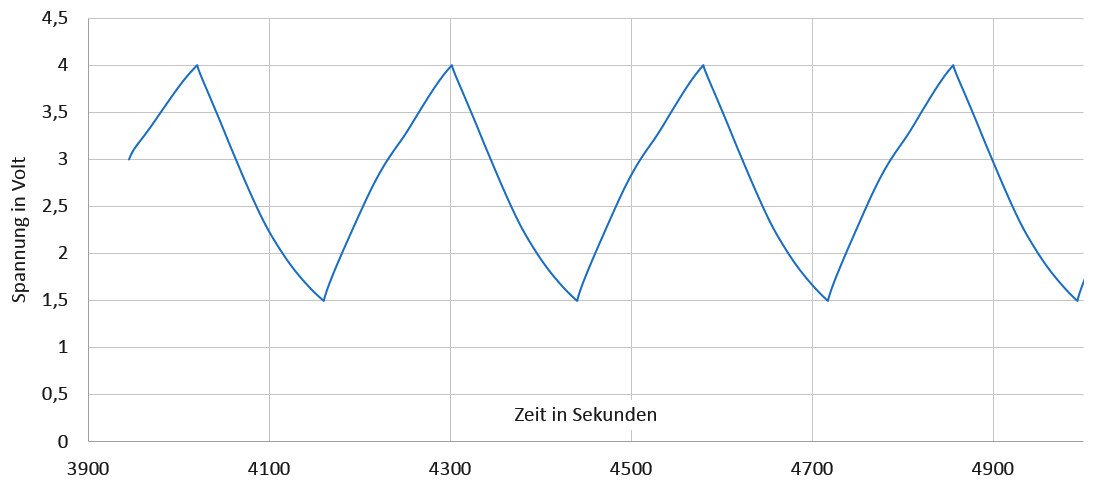
\includegraphics[width=1.00\columnwidth]{images/GCPL_LAGP.jpg}
	\label{gcpl_LAGP}
	} \vspace{3mm}
      \subfloat[Zyklische Voltametrie]{
	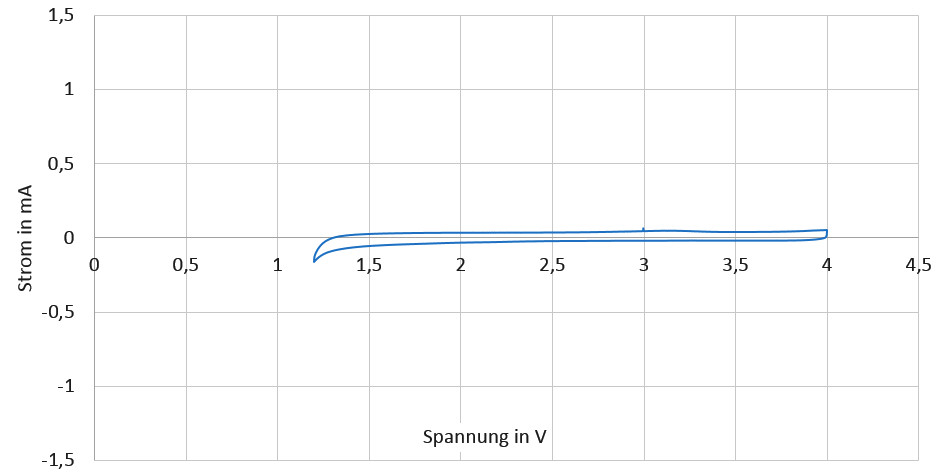
\includegraphics[width=0.85\columnwidth]{images/CV_LAGP.jpg}
	\label{cv_LAGP}   
      	} \vspace{3mm}
      \subfloat[Impedanzspektroskopie]{
	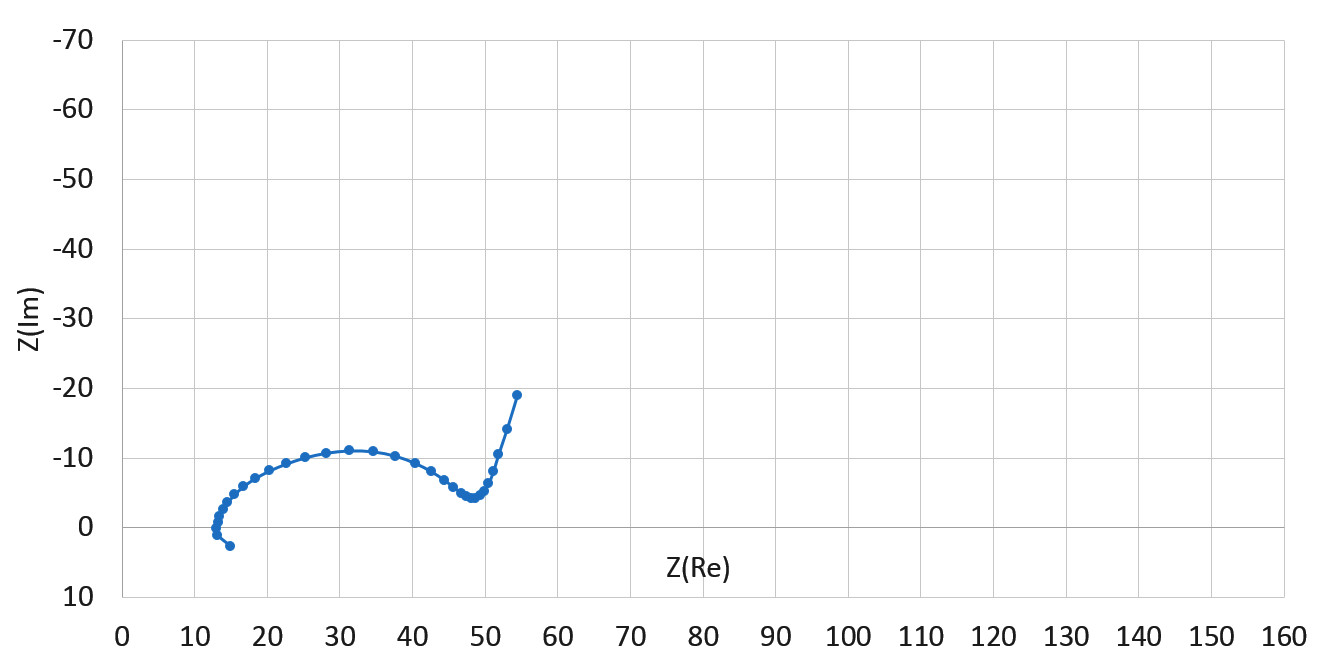
\includegraphics[width=0.85\columnwidth]{images/IS_LAGP.jpg}
	\label{is_LAGP}    
      	} \vspace{3mm}
	\caption{Charakterisierung des LAGP mit (a)~Ladekennlinie, (b)~Zyklischer Voltametrie, (c)~Impedanzspektroskopie}
   	\label{ec_LAGP}
\end{figure}
Der Spannungsbereich für die Zyklierung der LAGP-Probe lag zwischen 1,5V und 4,0V. In der zyklischen Voltametrie wurde ein Spannungsbereich von 1,2V bis 4,0V abgefahren.
\subsubsection{Ladekennlinien}
In der Lade- und Entladekennlinie der LAGP-Probe in Abbildung \ref{gcpl_LAGP} ist ein Sägezahnmuster zu erkennen. Es bilden sich weder beim Laden noch beim Entladen Plateaus aus. zwischen Beginn und Ende von Lade- und Entladevorgang liegen jeweils nur knapp 140 Sekunden.
\\\\
Daraus ergibt sich eine abgegebene Ladung während des Entladevorgangs von 1,94$\mu$Ah. Bei einem Gewicht des Aktivmaterials von 0,47mg entspricht dies einer Kapazität von 4,13mAh.
\subsubsection{Zyklische Voltametrie}
Die zyklische Voltametrie der LAGP-Probe, dargestellt in Abbildung \ref{cv_LAGP}, zeigt keinerlei Peaks der Stromstärke, egal welche Spannung angenommen wird.
\subsubsection{Impedanzmessungen}
Eine Darstellung der Impedanzmessung der LAGP-Probe in Nyquist-Darstellung wird in Abbildung \ref{is_LAGP} gezeigt. Im Graph sind zwei sich überschneidende Halbkreise sichtbar. Die X-Achse wird bei \SI{12}{\ohm} Realteil nahezu senkrecht geschnitten. Bei einem Realteil von \SI{49}{\ohm} geht der Halbkreis in eine Gerade mit einem Winkel von 75$^\circ$ zur X-Achse über.
\newpage
\subsection{LTO-Kathode}
\begin{figure}
   \centering
      \subfloat[Ladekennlinie]{
	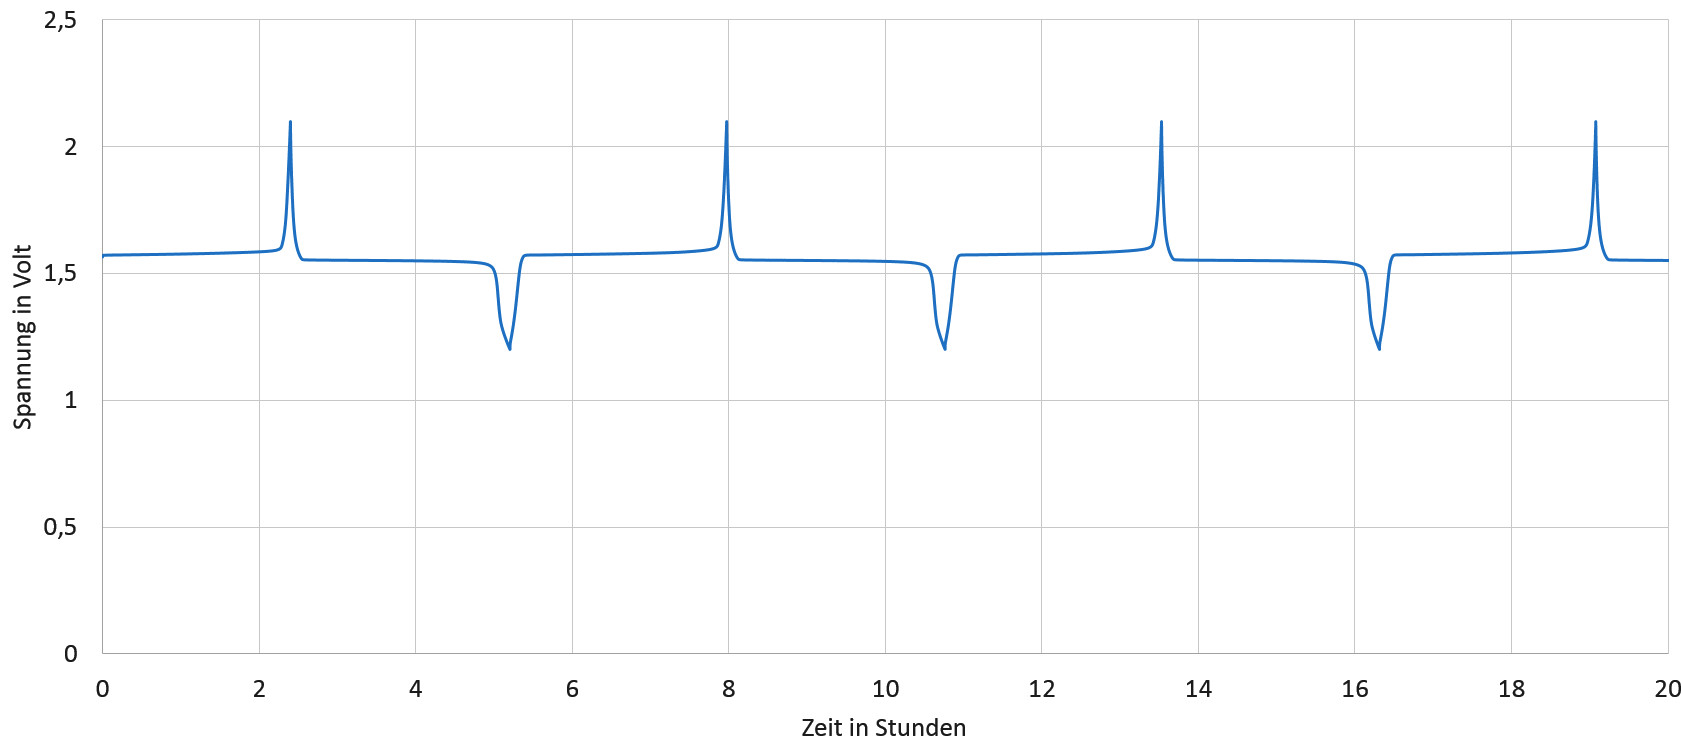
\includegraphics[width=1.00\columnwidth]{images/GCPL_LTO.jpg}
	\label{gcpl_LTO}
	} \vspace{3mm}
      \subfloat[Zyklische Voltametrie]{
	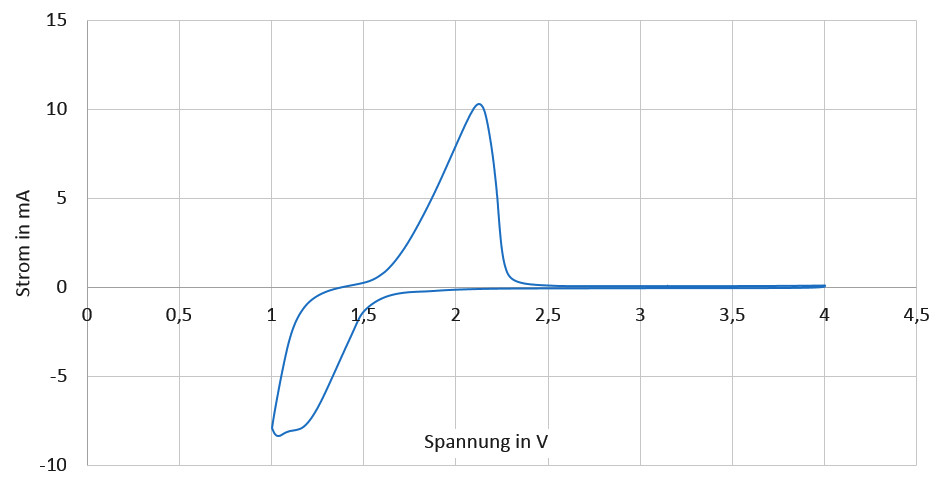
\includegraphics[width=0.85\columnwidth]{images/CV_LTO.jpg}
	\label{cv_LTO}   
      	} \vspace{3mm}
      \subfloat[Impedanzspektroskopie]{
	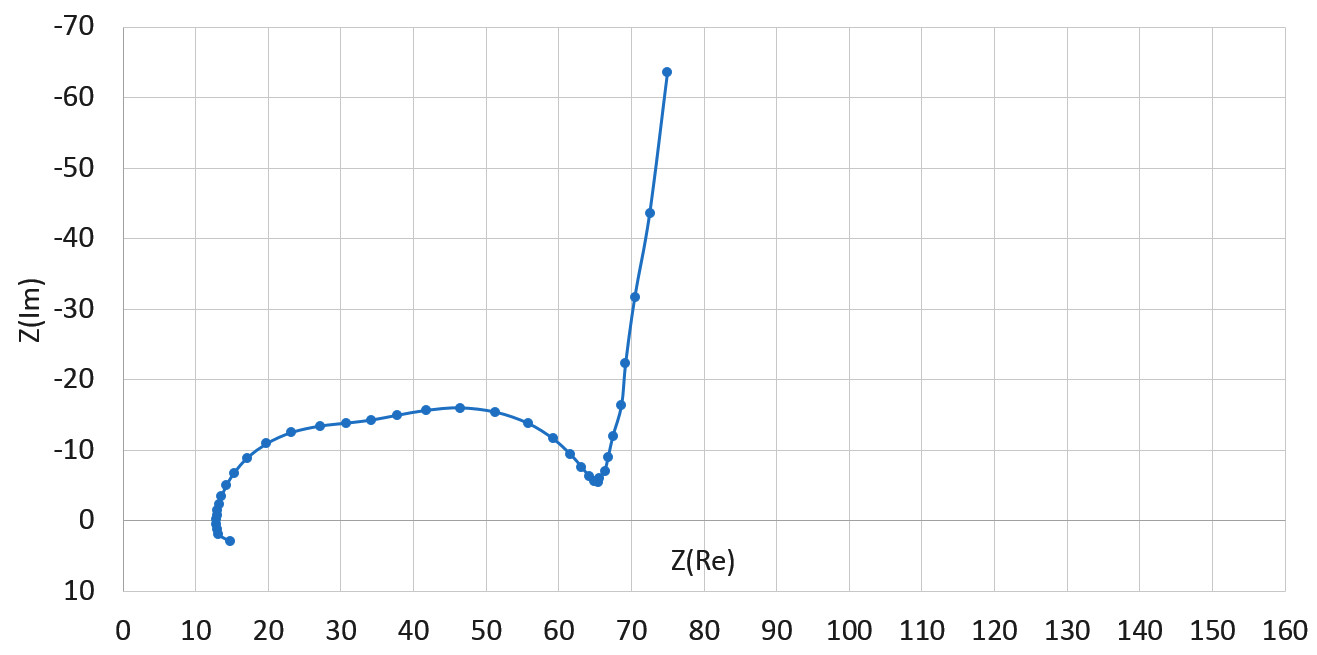
\includegraphics[width=0.85\columnwidth]{images/IS_LTO.jpg}
	\label{is_LTO}    
      	} \vspace{3mm}
	\caption{Charakterisierung des LTO mit (a)~Ladekennlinie, (b)~Zyklischer Voltametrie, (c)~Impedanzspektroskopie}
   	\label{ec_LTO}
\end{figure}
Die LTO-Probe wurde im Bereich zwischen 1,2V und 2,1V zykliert. Für die zyklische Voltametrie wurden als Grenzen 1,0V und 4,0V gewählt.
\subsubsection{Ladekennlinien}
Die Lade- und Entladekennlinie der LTO-Probe in Abbildung \ref{gcpl_LTO} zeigt sehr ausgedehnte Plateaus und scharfe Anstiege beziehungsweise Abfälle der Spannung vor dem Erreichen der Abbruchspannungen. Das Plateau beim Laden liegt bei 1,6V, das beim Entladen bei etwa 1,55V. Ein Lade- oder Entladevorgang dauert jeweils etwa 136 Minuten.
\\\\
Während des Entladevorgangs wurde Ladung in Höhe von 113,7$\mu$Ah abgegeben. Dividiert durch das Gewicht des Aktivmaterials von 0,61mg ergibt sich daher eine erreichte Kapazität von 186,4mAh/g.
\subsubsection{Zyklische Voltametrie}
Die zyklische Voltametrie der LTO-Probe zeigt zwei ausgeprägte Peaks. Zu sehen ist dies in Abbildung \ref{cv_LTO}. Der Peak auf dem ansteigenden Potantialast beginnt bei 1,5V und hat seinen Höhepunkt bei etwa 2,15V. Danach fällt er schnell ab. Im absteigenden Bereich beginnt der Peak bei etwa 1,5V und hat seinen Höhepunkt bei ungefähr 1,2V. Die Intensität beider Peaks ist sehr groß.
\subsubsection{Impedanzmessungen}
Die Impedanzmessung, dargestellt im Nyquist-Plot in Abbildung \ref{is_LTO}, der LTO-Kathoden\-probe zeigt zwei ineinander geschobene Halbkreise. Ab einem Realteil von \SI{66}{\ohm} gehen die Halbkreise in eine Gerade mit einem Winkel von 80$^\circ$ zur X-Achse über. Bei einem Realteil von \SI{12}{\ohm} trifft der Graph die X-Achse in einem senkrechten Winkel.
\newpage
\subsection{LLTO-Kathode}
\begin{figure}
   \centering
      \subfloat[Ladekennlinie]{
	\includegraphics[width=1.00\columnwidth]{images/GCPL_LLTO.jpg}
	\label{gcpl_LLTO}
	} \vspace{3mm}
      \subfloat[Zyklische Voltametrie]{
	\includegraphics[width=0.85\columnwidth]{images/CV_LLTO.jpg}
	\label{cv_LLTO}   
      	} \vspace{3mm}
      \subfloat[Impedanzspektroskopie]{
	\includegraphics[width=0.85\columnwidth]{images/IS_LLTO.jpg}
	\label{is_LLTO}    
      	} \vspace{3mm}
	\caption{Charakterisierung des LLTO mit (a)~Ladekennlinie, (b)~Zyklischer Voltametrie, (c)~Impedanzspektroskopie}
   	\label{ec_LLTO}
\end{figure}
Der Spannungsbereich für die Zyklierung der LLTO-Probe lag zwischen 0,8V und 4,2V. Als Lade- und Entladestrom wurde anstatt der sonst gewählten 50$\mu$A ein Strom von \SI{100}{\micro\ampere} angelegt. In der zyklischen Voltametrie wurde ein Spannungsbereich von 0,8V bis 4,2V abgefahren.
\subsubsection{Ladekennlinien}
Die Lade- und Entladekennlinie der LLTO-Kathodenprobe weist mehrere Bereiche auf. Sie wird in Abbildung \ref{gcpl_LLTO} dargestellt. Während des Ladevorgangs kann zwischen einem Bereich zwischen \SI{0.8}{\volt} bis \SI{1.0}{\volt}, einem Bereich mit höhrere Steigung zwischen \SI{1.0}{\volt} bis \SI{1.4}{\volt} und einem Bereich über \SI{1.4}{\volt} unterschieden werden. Im Entladefall existieren die Bereiche zwischen \SI{1.4}{\volt} und \SI{1.0}{\volt} sowie zwischen \SI{1.0}{\volt} und \SI{0.8}{\volt} reversibel zum Ladefall. Die Bereiche unter \SI{1.0}{\volt} sind dabei auf eine Zyklierung des Graphits innerhalb des Leitrußes zurückzuführen. Insgesamt benötigt ein Ladevorgang 28 Minuten, ein Entladevorgang 26,5 Minuten. Ohne die Bereiche unter \SI{1.0}{\volt} sind es 20 respektive 13 Minuten.
\\\\
Für den graphitfreien Fall  wird während eines Entladevorgangs \SI{22.2}{\micro\ampere\hour} Ladung abgegeben. Bei einem Gewicht des Aktivmaterials von 0,50mg entspricht das einer erreichten Kapazität von 44,4mAh/g.
\subsubsection{Zyklische Voltametrie}
Die zyklische Voltametrie in Abbildung \ref{cv_LLTO} zeigt im ansteigenden Potentialbereich zwei Peak bei \SI{1.05}{\volt} und \SI{1.55}{\volt}. Der erste Peak dürfte dabei der Graphitzyklierung zuzuordnen zu sein.  Im Bereich zwischen \SI{3.5}{\volt} und \SI{4.0}{\volt} existiert außerdem noch ein Plateau mit leichter Steigung. Im absteigenden Potentialast ist neben dem graphitischen Übergangspeak bei \SI{0.8}{\volt} ein Peak bei etwa \SI{1.0}{\volt} zu erkennen.
\subsubsection{Impedanzmessungen}
die Impedanzmessung in Abbildung \ref{is_LLTO} zeigt zwei sich überlappende Halbkreise, die bei einem Realteil von \SI{52}{\ohm} in eine Gerade mit einem Winkel von \SI{80}{\degree} zur X-Achse übergeht. Der Schnitt mit der X-Achse erfolgt bei \SI{12}{\ohm} Realteil im senkrechten Winkel.
\newpage
\subsection{LTO-LLTO-Gefüge}
\begin{figure}
	\centering
	\includegraphics[width=1.00\columnwidth]{images/IS_Gefuege.jpg}
	\caption{Gemessenes Impedanzspektrum (blau) und angefitteter Halbkreis (orange) für die LTO-LLTO-Li-Zelle}
	\label{is_Gefuege}
\end{figure}
Die Gefügeprobe zeigt schon bei sehr kleinen angelegten Lade- und Entladeströmen im Nanoampere-Bereich extrem hohe resultierende Spannungen. Eine Zyklierung konnte daher nicht stattfinden.
\subsubsection{Impedanzmessungen}
Für die Impedanzmessungen der Gefügeprobe wurde die Spannung der Sinusamplitude auf \SI{100}{\milli\volt} angehoben. Die Anzahl der Messpunkte pro Zehnerpotenz wurde ebenfalls erhöht auf 20. Bei Widerständen über \SI{10}{\mega\ohm} waren mit dem zum Einsatz kommenden VMP3-Messsystem keine fehlerfreien Messungen mehr möglich.
\\\\
Abbildung \ref{is_Gefuege} zeigt das gemessene Impedanzspektrum. Es kann dabei ein Halbkreis an die fehlerbehaftete Messung angefittet werden. Dieser trifft die X-Achse bei einem Realteil von \SI{10}{\kilo\ohm} und \SI{36.5}{\mega\ohm}. An beiden Stellen beträgt der Innenwinkel zur X-Achse dabei \SI{75}{\degree}
\newpage
\section{In-situ NMR-Messungen}
Für die in-situ NMR-Messungen werden zunächst die angefertigten Bauteile mittels einer Lithiumchlorid-Lösung kalibriert. Anschließend wird mit einer Lithium-Schwefel-Zelle die Funktionsfähigkeit des Messaufbaus gezeigt. Die Wahl des Zellmaterials fiel dabei auf Lithium-Schwefel, da es hierfür bereits ausreichend Ergebnisse in der Literatur und auch erste Voruntersuchungen im Rahmen einer Studienarbeit am IAM-KWT gibt.
\subsection{Referenzmessung}
Um das Spektroskop zu kalibrieren wurden zunächst Referenzmessungen mit einer Lithium\-chlorid-Lösung durchgeführt. Dazu wurde Lithiumchlorid (FIRMA) im Masseverhältnis $1:2$ in Wasser gelöst. Die Lösung wurde sowohl in ein handelsübliches 10mm NMR-Röhrchen als auch in eine Batterietestzelle eingefüllt. In der Zelle wurden dabei vier Lagen Separator mit der Lösung benetzt, um die Flüssigkeit im Messbereich zu halten.
\subsubsection{Einstellen der Geräteparameter}
\begin{table}[b]
\centering
\begin{tabular}{L{5.0cm} L{5.0cm}}
\toprule
 \textbf{Parameter}&\textbf{Wert} \\
\midrule
Datenpunkte pro Scan& 16384\\
\midrule
Bandbreite& \SI{2.5}{\kilo\hertz}\\
\midrule
Receiver Gain& 11,3\\
\midrule
Dwell Time& \SI{40}{\micro\sec}\\
\midrule
Todzeit& \SI{6}{\micro\sec}\\
\midrule
D1& \SI{5}{\sec}\\
\midrule
Pulslänge (0db)& \SI{12}{\micro\sec}\\
\bottomrule
\end{tabular}
 \caption{Parameter für das Messen des Kalibrierspektrums mit der LiCl-Lösung}
 \label{tabelle_parameter_nmr}
\end{table} 
Die modifizierte Spule (siehe Kapitel \ref{anpassung_probenkopf}) wird auf den Probenkopf montiert. Die Referenzproben können dann einfach in die Teflonröhre eingeführt werden. Anschließend wird der gesamte Probenkopf von unten in das NMR-Gerät eingeführt und fixiert. Der Probenkopf wird händisch auf die richtige Frequenz grobabgestimmt. Dazu können an der Unterseite des Probenkopfs mittels Drehreglern kleine variable Kondensatoren in ihrer Kapazität variiert werden. In einem nächsten Schritt kann über die Ansteuerung am Rechner das Signal über die Homogenisierung des Magnetfeldes feinabgestimmt werden.
\\\\
Nachdem das Signal angepasst worden ist, können möglichst optimale Parameter für die eigentlichen Messungen gesucht werden. Dazu werden unterschiedliche Messparameter variiert und die Auswirkung der Änderung auf die gemessene Probespektren beobachtet. Ziel ist es hierbei, die Parameter so zu wählen, dass das Rauschen der Messung möglichst klein ist. Weiterhin muss eine Bandbreite gefunden werden, die alle relevanten Peaks der Messung darstellt. Unter einer zu großen Bandbreite leidet die Qualität der Messung. Die Anzahl an Datenpunkten, Scans und Messzeiten pro Scan kann die Qualität der Messung verbessern, erhöht allerdings auch drastisch die Messzeit. Hier muss ein guter Mittelweg gefunden werden. Die für die Referenzprobe verwendeten Werte werden in Tabelle \ref{tabelle_parameter_nmr} dargestellt.
\subsubsection{Spektrum der Referenzproben}
\begin{figure}
	\centering
	\includegraphics[width=0.75\columnwidth]{images/LiCl_Batterie.jpg}
	\label{LiCl_Batterie_NMR} 
	\caption{Spektrum der LiCL-Lösung innerhalb der Batterietestzelle}
	\label{LiCl_Batterie_NMR}
\end{figure} 
Die Spektren der beiden Referenzproben zeigen beide einen deutlichen und scharfen Peak der Lithiumionen. Auf diesen Peak kann das Gerät für die weiteren Messungen eingestellt werden, so dass dieser den Nullpunkt der Messung darstellt. Abbildung \ref{LiCl_Batterie_NMR} zeigt das Spektrum der Lithiumchlorid-Lösung innerhalb der Batterietestzelle.
\subsubsection{Diffusionsmessungen}
\begin{figure}
   \centering
      \subfloat[Diffusionsmessung  der LiCl-Lösung in einem NMR-Röhrchen]{
	\includegraphics[width=0.95\columnwidth]{images/LiCl_Diff.jpg}
	\label{LiCl_Diff}
	} \vspace{10mm}
      \subfloat[Diffusionsmessung der LiCl-Lösung in der Batterietestzelle]{
	\includegraphics[width=0.95\columnwidth]{images/LiCl_Diff_Batterie.jpg}
	\label{LiCl_Diff_Batterie}      
      	} \vspace{6mm}
	\caption{Vergleich der Diffusionsmessung der LiCl-Lösung in einem NMR-Röhrchen und in der Batterietestzelle. Dargestellt werden die Resonanzen für die unterschiedlichen Feldstärken.}
   	\label{vergleich_diff}
\end{figure}
Für die Referenzproben wurden Diffusionsmessungen durchgeführt. Die Darstellungen in Abbildung \ref{vergleich_diff} visualisieren dabei das Ergebnis der Messung. Zu erkennen ist, dass der Messaufbau die Diffusionsmessung verrauscht. Es ist jedoch immer noch gut möglich, die Diffusion zu bestimmen. Der so ermittelte Diffusionskoeffizient für die Lithiumchlorid-Lösung betrug im NMR-Röhrchen  \SI{2.825e-10}{\square\meter\per\sec}, in der Batterie bei  \SI{2.593e-10}{\square\meter\per\sec}.
\subsection{Lithium-Schwefel-Zelle}
\begin{figure}
	\centering
	\includegraphics[width=0.85\columnwidth]{images/GCPL_LiS.jpg}
	\caption{Lade-/Entladekennlinie der Lithium-Schwefel-Testzelle}
	\label{gcpl_LiS}
\end{figure} 
Für die in-situ-NMR-Batterietestzelle wurde eine Lithium-Schwefel-Zelle gebaut. Dies erfolgte äquivalent zum im Kapitel \ref{bau_zellen} vorgestellten Verfahren für die herkömmlichen Batterietestzellen. Die Größe der Elektroden und der Separatoren wurde auf einen Durchmesser von \SI{6}{\milli\meter} verringert. Als Elektrolyt kamen \SI{20}{\micro\liter} einer ???-Lösung zum Einsatz. Vor dem Einbau in das NMR-Spektroskop wird die Zelle zweimal zykliert. Abbildung \ref{gcpl_LiS} zeigt die Ladekennlinie der Zelle. Zu erkennen sind die unterschiedlichen Lade- und Entladeplateaus der Zelle, die auf die unterschiedlichen Sulfidationsschritte des Lithiums zurückzuführen sind.
\\\\
Mit der Lithium-Schwefel-Testzelle wurden drei Messungen durchgeführt. Es wurde jeweils ein NMR-Spektrum vor und nach einer 90 minütigen Ladephase aufgenommen. Geladen wurde mit einem Strom von \SI{50}{\micro\ampere}. Außerdem wurde vor dem Ladevorgang eine Diffusionsmessung durchgeführt.
\subsubsection{Spektren der LiS-Testzelle}
\begin{figure}
   \centering
      \subfloat[Spektrum der Lithium-Schwefel-Zelle vor dem Laden]{
	\includegraphics[width=0.75\columnwidth]{images/LiS_VorLaden.jpg}
	\label{LiS_VorLaden}
	} \vspace{10mm}
      \subfloat[Spektrum der Lithium-Schwefel-Zelle nach 90 minütigem Laden]{
	\includegraphics[width=0.75\columnwidth]{images/LiS_NachLaden.jpg}
	\label{LiS_NachLaden}      
      	} \vspace{6mm}
	\caption{Spektren der in-situ-NMR-Batterietestzelle}
   	\label{insitu_nmr}
\end{figure}  
Das Spektrum der Lithium-Schwefel-Testzelle zeigt in Abbildung \ref{LiS_VorLaden} zwei Peaks. Einen großen, scharfen Peak auf dem geeichten Lithiumionen-Punkt von 0\;ppm sowie einen breiteren und weniger starken Peak bei etwa 245\;ppm. Dieser ist dem Lithiummetall zuzuordnen.
\\\\
Nach dem 90 minütigem Laden zeigt sich in Abbildung \ref{LiS_NachLaden} ein deutliche Vergrößerung des Peaks des metallischem Lithiums. Außerdem haben sich zwei weitere, weniger intensive Peaks in unmittelbarer Nähe zum Lithiumionen-Peak gebildet. Diese sind in die negative Richtung verschoben und könnten Übergangsprodukte des Ladeprozesses darstellen.
\subsubsection{Diffusionsmessung}
Die Diffusionsmessung an der Lithium-Schwefel-Testzelle zeigt ein starkes Rauschen. Abbildung \ref{LiS_Diff} zeigt die zugehörige Darstellung. Der Diffusionskoeffizient konnte bestimmt werden zu \SI{6,34e-11}{\square\meter\per\sec}.
\begin{figure}
	\centering
	\includegraphics[width=0.95\columnwidth]{images/LiS_Diff_Batterie.jpg}
	\caption{Diffusionsmessung der LiS-Batterietestzelle}
	\label{LiS_Diff}
\end{figure} 
%%%%%%%%%%%%%%%%% 6. DISKUSSION %%%%%%%%%%%%%%%%%

\chapter{Diskussion}
Die im vorherigen Kapitel erhaltenen Ergebnisse der elektrochemischen Untersuchung ermöglichen Rückschlüsse auf die Eignung der Materialien als Festkörperelektrolyt. Die Ladekennlinien ermöglichen eine Aussage über den Grad der Reaktion des Materials mit dem Lithium. Mit der zyklischen Voltametrie sind Aussagen über mögliche Arbeitsspannungen für die Materialien möglich. Für die Impedanzspektroskopie wird ein elektrochemisches Ersatzschaltbild motiviert. Mit diesem werden Aussagen über Grenzschichten und Diffusionsverhalten der Zellen getroffen.
\\\\
Für die Kernspinresonanzspektroskopie wird die grundsätzliche Eignung der Technik sowie des angefertigten Messsystems diskutiert. % Hier noch mehr
\section{Diskussion der elektrochemischen Untersuchung}
Um zu verstehen, ob und wie die untersuchten Materialien mit dem Lithium der Zelle reagieren, können Ergebnisse der elektrochemischen Untersuchung der Proben analysiert werden. Dabei wird insbesondere die Menge und der Zeitpunkt des Einbaus von Lithium in das Material untersucht. Weiterhin können mit der Impedanzspektroskopie die Grenzschicht und das Diffusionsverhalten der Probe genauer beschrieben werden.
\subsection{Vergleich der Zellkapazitäten und des Ladeverhaltens}
\begin{figure}
	\centering
	\includegraphics[width=1.00\columnwidth]{images/kapazitaeten.jpg}
	\caption{Übersicht über die verschiedenen Kapazitäten der untersuchten Keramiken (in mAh/g)}
	\label{kapazitaeten}
\end{figure}
Die vier untersuchten Materialien weisen als Kathodenmaterial unterschiedlich hohe Kapazitäten auf. Eine hohe Kapazität bedeutet dabei, dass es während der Zyklierung zu einem starken Einbau von Lithium in das Material hinein gekommen sein muss. In einem Festkörperelektrolyten sollten die Lithiumionen jedoch nur durchgeleitet, nicht eingebaut werden. Eine starke Zyklierbarkeit des Elektrolytmaterials ist daher nicht wünschenswert. Eine Übersicht über die Kapazitäten der vier untersuchten Materialien findet sich in Abbildung \ref{kapazitaeten}.
\\\\
Die höchste Kapazität erreicht das klassische Anodenmaterial LTO mit \SI{186}{\milli\ampere\hour\per\gram}. Dies liegt nur knapp \SI{20}{\percent} unter der maximalen theoretischen Kapazität des Materials von \SI{233}{\milli\ampere\hour\per\gram} und deutlich über der normal erreichbaren praktischen Kapazität in kommerziellen Zellen von \SI{150}{\milli\ampere\hour\per\gram}. Die Stärke des Ein- und Ausbaus von Lithium spricht daher gegen seine Verwendung als Festkörperelektrolyt.
\\\\
Das LATP und das LLTO besitzen beide moderate Kapazitäten. Die LATP-Probe kommt dabei auf eine Kapazität von \SI{61}{\milli\ampere\hour\per\gram}, die LLTO-Probe auf \SI{44}{\milli\ampere\hour\per\gram}. Als Elektrodenmaterial eignen sich beide Keramiken damit nicht, ihre Kapazitäten liegen um einen Faktor von mehr als drei unter dem der LTO-Probe und anderen vergleichbaren Materialien. Um als Festkörperelektrolyt eingesetzt werden zu können, muss die Reaktion mit dem Lithium besser eingedämmt werden. 
\\\\
Mit nur \SI{4}{\milli\ampere\hour\per\gram} erreicht das LAGP quasi keine Kapazität. Es ist also nicht zu einem starken Ein- und Ausbau von Lithiumionen während der Zyklierung gekommen. Damit erfüllt das LAGP in den zyklierten Spannungsbereichen die nötigen Stabilitätsbedingungen für einen Einsatz als Festkörperelektrolyt.
\subsubsection{Analyse des Kapazitätsverlustes}
\begin{figure}
	\centering
	\includegraphics[width=1.00\columnwidth]{images/kapazitaetsverlust.jpg}
	\caption{Relativer Verlust der Kapazität über elf Zyklierungen}
	\label{kapazitaetsverlust}
\end{figure}
Während der Zyklierung kommt es auch zu einem Verlust an Kapazität. Dieser Verlust ist ein Maß für die Degradierung des Materials. Durch ungewollte Nebenreaktionen entwickeln die Elektrodenmaterialien passivierte Schichten, die dann verhindern, dass Material an der Zyklierung teilnimmt. Eine Übersicht über den Verlust an Kapazität gibt Abbildung \ref{kapazitaetsverlust}. Zu erkennen ist, dass die LTO- und die LAGP-Probe jeweils nur knapp \SI{3}{\percent} ihrer ursprünglichen Kapazität verlieren und sich auf diesem Niveau auch stabilisieren. Das LLTO sowie das LATP hingegen haben nach elf Zyklierungen schon über \SI{10}{\percent} ihrer ursprünglichen Kapazität verloren. Dieser Trend scheint sich außerdem auch noch weiter fortzusetzen.
\subsection{Analyse der Lithiuminsertation}
Mittels der molaren Masse einer Struktureinheit können die Kapazitäten der untersuchten Materialien umgerechnet werden zur Anzahl der pro Struktureinheit eingebauten Lithium\-ionen. Ein Lithiumion besitzt eine einfache elektrischen Ladung, was \SI{1.602e-19}{\coulomb} entspricht. Ein Coulomb sind umgerechnet \SI{0.28}{\milli\ampere\hour}. Mit der Avogadrozahl lässt sich damit die Ladung pro Mol bestimmen zu \SI{26.8}{\ampere\hour\per\mol}.
\\\\
Die Ergebnisse dieser Berechnung für die untersuchten Materialien lassen sich in Tabelle \ref{berechnung_insertation} finden. Es fällt auf, dass pro Struktureinheit in das LATP beinahe dreimal mehr Lithium\-ionen eingebaut werden, als in das LLTO. Das LAGP bleibt wie zu erwarten nahezu frei von Insertation, das LTO baut mehr als drei Ionen pro Struktureinheit ein.
\\
\begin{table}[h]
\begin{tabular}{L{1.3cm} L{3.5cm} L{3.5cm} L{2.4cm} L{2.6cm}}
\toprule
&\textbf{LATP}&\textbf{LAGP}&\textbf{LTO}&\textbf{LLTO} \\
\midrule
\textbf{SE} & \ce{Li_{1,3}Al_{0,3}Ti_{1,7}(PO4)3} & \ce{Li_{1,3}Al_{0,3}Ge_{1,7}(PO4)3} & \ce{Li4Ti5O12} & \ce{Li_{0,33}La_{0,577}TiO3} \\
\midrule
\textbf{M} & \SI{383.8}{\gram\per\mol}& \SI{425,5}{\gram\per\mol}& \SI{459.1}{\gram\per\mol}&  \SI{175,5}{\gram\per\mol}\\
\midrule
\textbf{C} & \SI{61.3}{\milli\ampere\hour\per\gram} &  \SI{4.13}{\milli\ampere\hour\per\gram} & \SI{186.4}{\milli\ampere\hour\per\gram}&  \SI{44.4}{\milli\ampere\hour\per\gram}\\
\midrule
\textbf{C/M} & \SI{23.53}{\ampere\hour\per\mol} & \SI{1.76}{\ampere\hour\per\mol}& \SI{85.58}{\ampere\hour\per\mol}&  \SI{7.79}{\ampere\hour\per\mol}\\
\midrule
\textbf{Li$^+$/SE} & 0,878 & 0,066 & 3,193 & 0,291\\
\bottomrule
\end{tabular}
\caption{Eingebaute Lithiumionen pro Struktureinheit (SE)}
\label{berechnung_insertation}
\end{table}

\subsection{Vergleich der möglichen Arbeitsspannungen}
Durch das gezielte Setzen eines Arbeitsspannungsbereichs, kann der Ein- und Ausbau der Lithiumionen verhindert werden. Damit ist es möglich, dass auch die Proben, die während der Zyklierung aktiv waren, für den Einsatz als Festkörperelektrolyt nutzbar gemacht werden können. Wichtig ist dabei das Zusammenspiel zwischen Arbeitsspannungsbereich der Elektroden und dem Arbeitsspannungsbereich des Elektrolyts.
\\\\
Mit der zyklische Voltametrie kann visualisiert werden, in welchen Bereichen die untersuchten Elektrolytmaterialen keine Reaktionen mit dem Lithium eingingen. Dort bilden sich keine Peaks aus, die Stromstärke liegt nahe Null. Tabelle \ref{spannung_keramiken} zeigt die aus den Daten der zyklischen Voltametrie in Kapitel \ref{elektrochemische_analyse} gewonnenen Arbeitsspannungsbereiche für das Laden und Entladen der Zelle.
\\
\begin{table}[h]
\begin{tabular}{L{2.6cm} L{2.6cm} L{2.6cm} L{2.6cm} L{2.6cm}}
\toprule
&\textbf{LATP}&\textbf{LAGP}&\textbf{LTO}&\textbf{LLTO} \\
\midrule
\textbf{Ladung} &\SI{1.2}{\volt} - \SI{2.3}{\volt}&\SI{1.2}{\volt} - \SI{4.0}{\volt}& \SI{2.8}{\volt} - \SI{4.0}{\volt}& \SI{1.7}{\volt} - \SI{3.3}{\volt}\\
\midrule
\textbf{Entladung} &\SI{4.0}{\volt} - \SI{2.7}{\volt} &\SI{4.0}{\volt} - \SI{1.2}{\volt}&\SI{4.0}{\volt} - \SI{1.6}{\volt}&  \SI{4.0}{\volt} - \SI{1.5}{\volt}\\
\bottomrule
\end{tabular}
\caption{Arbeitsspannungsbereiche der untersuchten Elektrolyt\-materialien}
\label{spannung_keramiken}
\end{table}
\\
Zu erkennen ist, dass es beim LATP nur einen sehr kleinen Arbeitsbereich für die Zyklierung gibt. Die Bereiche für Laden und Entladen überlappen außerdem nicht, weshalb in grundsätzlich ungünstigen Bereichen zykliert werden muss. Das LAGP zeigt über den gesamten abgefahrenen Spannungsbereich keine Reaktionen. Damit scheint es innerhalb dieses Bereiches stabil zu sein und eignet sich in diesem Kriteriung für den Einsatz mit einer Vielzahl von unterschiedlichen Anoden- und Kathodenmaterialien.
\\\\
Das LTO besitzt für das Laden eine maximale Spannung von \SI{4.0}{\volt}, welches jedoch bei mindestens \SI{2.8}{\volt} beginnen muss. Das Entladen kann bis \SI{1.6}{\volt} durchgeführt werden. Beim LLTO darf die maximale Ladespannung nicht über \SI{3.3}{\volt} liegen und muss bei mindestens \SI{1.7}{\volt} beginnen. Die Zelle kann bis \SI{1.5}{\volt} entladen werden. Damit eignet sich das LLTO grundsätzlich für den Einsatz als Elektrolyt in diesem Bereich.
% Für alle untersuchten Materialien gilt, dass ...
\subsection{Entwicklung eines elektrochemischen Ersatzschaltbilds}
Zur besseren Interpretation der Impedanzspektroskopie kann ein elektrochemisches Ersatzschaltbild entwickelt werden. Dafür soll mittels der Verteilung der Relaxationszeiten (Distribution of Relaxation Times, DRT) zunächst das Spektrum auf die Anzahl detektierbarer Mechanismen untersucht werden. Anschließend werden zwei unterschiedliche Modelle auf Basis der Daten entwickelt.
\subsubsection{DRT}
Für die DRT-Analyse kommt ein am IAM-KWT entwickeltes Labview-Programm zum Einsatz. Dabei konnten mit Ausnahme des LATP für jede der vier untersuchten Elektroden jeweils zwei Prozesse gefunden werden. Das LATP weist nur einen Prozess auf. Dies steht in Einklang mit den in Kapitel \ref{elektrochemische_analyse} gefunden Halbkreisen innerhalb der Impedanzspektren. Die ermittelten Frequenzen dieser Prozesse lassen sich in Tabelle \ref{tabelle_drt} finden.
\\
\begin{table}[h]
\begin{tabular}{L{5.2cm} L{2.0cm} L{2.0cm} L{2.0cm} L{2.0cm}}
\toprule
&\textbf{LATP}&\textbf{LAGP}&\textbf{LTO}&\textbf{LLTO} \\
\midrule
\textbf{Frequenz erster Prozess} &\SI{3.42}{\kilo\hertz}&\SI{3.98}{\kilo\hertz}& \SI{1.36}{\kilo\hertz}& \SI{0.54}{\kilo\hertz}\\
\midrule
\textbf{Frequenz zweiter Prozess} & - &\SI{29.29}{\kilo\hertz}&\SI{10.00}{\kilo\hertz}&  \SI{4.64}{\kilo\hertz}\\
\bottomrule
\end{tabular}
\caption{Ergebnis der DRT-Analyse}
\label{tabelle_drt}
\end{table}
\subsubsection{Reihenmodell}
Eine Batterie kann als Verkettung mehrerer Grenzschichten gesehen werden. Diese sind beispielsweise die Grenzschicht zwischen Elektrode und Elektrolyt oder zwischen Elektrode und Stromkollektor. Eine solche Grenzschicht baut jeweils ein kapazitives Element in Form einer Helmholtz-Doppelschicht auf und besitzt einen Durchtrittswiderstand. Schaltet man diese zwei Elememente parallel zueinander, so erhält man ein RC-Glied. Dieses bildet im Nyquist-Plot einen perfekten Halbkreis. Nun kann an den erhaltenen Spektren gesehen werden, dass die gemssenen Halbkreise teilweise verschoben und verdrückt vorliegen. Ihre Winkel zur x-Achse entsprechen größtenteils nicht den zu erwartenden \SI{90}{\degree}. Dies ist darin begründet sein, dass die Kapazität der Grenzschichten nicht ideal ist. Daher werden die Kondensatoren durch Q-Elemente ersetzt, welche dieses nicht-ideale Verhalten modellieren können. Das entsprechende Bauteil für Grenzschichten im Modell ist dann das RQ-Glied.
\\\\
In der DRT-Messung und in den Impedanzspektren konnten jeweils nur ein oder zwei Prozesse in jeder Zelle gefunden werden. Die Anzahl der RQ-Glieder wird daher auf diese Menge gesetzt. % Mehr Begündung
\\\\
Die Diffusion des Lithiums durch die Elektroden hindurch kann in der metallischen Lithiumanode als ideal und vernachlässigbar angenommen werden. Für die Kathode kann der Diffusionsprozess mittels eines Warburg-Elements modelliert werden. Dieses stellt als Verkettung mehrerer RC-Glieder die Hindernisse und Ladungsbarrieren beim Transport durch das Material dar.
\\\\
Die Batterie besitzt außerdem noch, bedingt durch den Testaufbau, Kabel, Stempel und auch dem Elektrolyten, einen inneren Widerstand. Verschaltet man diesen nun mit den zwei RQ-Gleidern für die Grenzschichten und dem Warburg-Element, so erhält man das in Abbildung \ref{schaltbild_2RQ} dargestellte Reihenmodell als elektrochemisches Ersatzschaltbild für die untersuchten Zellen. 
\begin{figure}
   \centering
      \subfloat[Reihenmodell]{
	\includegraphics[width=0.7\columnwidth]{images/Schaltbild_2RQ.png}
	\label{schaltbild_2RQ}
	} \vspace{10mm}
      \subfloat[Redox-Modell]{
	\includegraphics[width=0.7\columnwidth]{images/Schaltbild_Randles.png}
	\label{schaltbild_Randles}      
      	} \vspace{6mm}
	\caption{Elektrochemisches Ersatzschaltbild des Reihen- sowie des Redox-Modells}
   	\label{ersatzschaltbilder}
\end{figure} 
\subsubsection{Redox-Modell}
Anstatt einer reinen Verkettung von RQ- und Warburg-Elementen, können diese auch teilweise parallel geschaltet werden. %Erklärung?
\\\\
Das entsprechende elektrochemische Ersatzschaltbild wird in Abbildung \ref{schaltbild_Randles} dargestellt.
\subsection{Auswertung der Impedanzspektroskopie}
Mit den aufgestellten Modellen wurden anschließend Fits zu den realen Messungen angefertigt und deren Güte und Aussagekraft untersucht.
\begin{table}[h]
\begin{tabular}{L{1.95cm} L{1.35cm} L{0.75cm} L{1.35cm} L{0.75cm} L{1.35cm}L{0.75cm}L{1.3cm}L{0.75cm}L{0.75cm}}
\toprule
&&\multicolumn{2}{c}{\textbf{LATP\;\;\;}}& \multicolumn{2}{c}{\textbf{LAGP\;\;\;}}&\multicolumn{2}{c}{\textbf{LLTO\;\;\;}}&\multicolumn{2}{c}{\textbf{LTO}}\\
& Modell & Reihe & Redox & Reihe & Redox & Reihe & Redox & Reihe & Redox\\
\midrule
\textbf{Widerstand}&R$_i$\;[$\Omega$]&9,29&9,36&12,44&13,59&12,55&12,78&12,94&13,03\\
\midrule
\multirowbt{3}{*}{\textbf{1.\;Glied}} & R$_1$\;[$\Omega$] & 72,00 & 69,82 & 20,18  & 7,85 & 12,24 & 16,97 & 18,51 & 23,62\\
\cmidrule{2-10}
 & C$_1$\;[\SI{}{\micro\farad}] & 0,74 & 0,71 & 0,69 & 0,36 & 0,83 & 0,55 & 1,25 & 0,97\\
\cmidrule{2-10}
 & f$_1$\;[\SI{}{\kilo\hertz}] & 18,89 & 20,25 & 71,34 & 356,35 & 98,87 & 108,5 & 43,13 & 43,48\\
\midrule
\multirowbt{3}{*}{\textbf{2.\;Glied}} & R$_2$\;[$\Omega$] & \quad- & \quad- & 13,05 & 26,12 & 24,77 & 21,76 & 33,94 & 29,34\\
\cmidrule{2-10}
 & C$_2$\;[\SI{}{\micro\farad}] & \quad - &  \quad- & 5,27 & 1,41 & 3,64 & 3,88 & 7,89 & 8,42 \\
\cmidrule{2-10}
 & f$_2$\;[\SI{}{\kilo\hertz}] &  \quad- &  \quad- & 14,53 & 27,14 & 11,10 & 11,83 & 3,73 & 4,05 \\
%\midrule
%\multirowbt{3}{*}{\textbf{Warburg}} & R$_W$\;[$\Omega$] & 133,1 & 9,7 & 10,5 & 7,3 & 8,0 & 3,2 &  & 1,1\\
%\cmidrule{2-10}
 %& C$_W$\;[\SI{}{\milli\farad}] & 1,3$\mu$F & 5,83 & 11,0 & 7,4 & 12,8 & 4,5 & 0,3$\mu$F & 1,8 \\
%\cmidrule{2-10}
% & f$_W$\;[\SI{}{\kilo\hertz}] &  &  &  & &&&&\\
\midrule
\textbf{Güte}&$\chi^2$[E-4]&1,47&1,39&3,09&0,74&2,27&1,78&3,83&3,42\\
\bottomrule
\end{tabular}
 \caption{Ergebnisse der Auswertung der Impedanzspektroskopie mit den zwei entwickelten Ersatzschaltbildern}
 \label{tabelle_is}
 \end{table} 
\begin{table}[h]
\begin{tabular}{L{1.4cm}L{2.2cm}  L{2.2cm} L{1.2cm} L{2.2cm}L{1.2cm}L{1.8cm}}
\toprule
&&\textbf{DRT\;\;\;}& \multicolumn{2}{c}{\textbf{Reihenmodell\;\;\;\;\;\;}}&\multicolumn{2}{c}{\textbf{Redoxmodell\;\;\;\;\;\;}}\\
\multicolumn{2}{l}{\qquad Frequenz in}&[\SI{}{\kilo\hertz}]&[\SI{}{\kilo\hertz}]&\% DRT&[\SI{}{\kilo\hertz}]&\% DRT\\
\midrule
\multirowbt{1}{*}{\textbf{LATP}} &1. Prozess&  3,42 & 18,89  & \SI{552}{\percent} & 20,25 &  \SI{592}{\percent}\\
\midrule
\multirowbt{2}{*}{\textbf{LAGP}} &1. Prozess&  3,98 & 14,53 & \SI{365}{\percent} & 27,14 &  \SI{682}{\percent}\\
\cmidrule{2-7}
& 2. Prozess & 29,29 & 71,34  & \SI{244}{\percent} & 356,35 & \SI{1217}{\percent}\\
\midrule
\multirowbt{2}{*}{\textbf{LLTO}} &1. Prozess &  1,36 & 11,10& \SI{816}{\percent} & 11,83 &  \SI{870}{\percent}\\
\cmidrule{2-7}
& 2. Prozess & 10,00 & 98,87 & \SI{989}{\percent} & 108,05 & \SI{1085}{\percent}\\
\midrule
\multirowbt{2}{*}{\textbf{LTO}} &1. Prozess&  0,54 & 3,73 & \SI{691}{\percent} & 4,05 & \SI{750}{\percent}\\
\cmidrule{2-7}
& 2. Prozess & 4,64 & 43,13 & \SI{930}{\percent} & 43,48 & \SI{937}{\percent}\\
\bottomrule
\end{tabular}
 \caption{Vergleich der Frequenzen zwischen DRT und Ersatzschaltbild-Fits}
 \label{tabelle_vergleich_frequenzen}
 \end{table} 
%\subsection{Vergleich des Diffusionsverhaltens}
\section{Diskussion der Kernspinresonanzspektroskopie}
Es wurde die MAS-NMR zur Pulvercharakterisierung eingesetzt. Für in-situ NMR-Messungen von Batterien wurde ein eigener Messaufbau konzipiert, konstruiert, gebaut und getestet. Im Folgenden soll die Anwendung und der Nutzen beider dieser Maßnahmen diskutiert werden. 
\subsection{Eignung der MAS-NMR für die Pulvercharakterisierung}
Die MAS-NMR kann nur eingeschränkt für die Pulvercharakterisierung eingesetzt werden. Versuche Fremdphasen wie das \ce{LiTiPO5} innerhalb des LATP zu detektieren, führten nicht zum Erfolg. Die Peaks beider Materialien überlagern sich und sind daher nicht zu separieren. Es konnte bei allen untersuchten Stoffen mittels Röntgendiffraktometrie genauere Aussagen über die Stoffzusammensetzung getroffen werden.
\\\\
% Paper zitieren
Dennoch kann die MAS-NMR Mehrinformationen bieten. Hierfür müsste allerdings nicht das Lithium-Isotop, sondern beispielsweise das Phosphor-Isotop untersucht werden. Verschiedene Forschungsgruppen konnten dabei Rückschlüsse auf die Struktur der untersuchten Keramiken ziehen (QUELLE).
\subsection{Funktionsfähigkeit des in-situ NMR-Testaufbaus}
\begin{figure}
   \centering
      \subfloat[Vergleich der LiCl-Referenz (rot) mit der LiS-Zelle (grün) vor dem Laden]{
	\includegraphics[width=0.75\columnwidth]{images/LiCl_LiS_Vergleich.jpg}
	\label{LiS_VorLaden_Vergleich}
	} \vspace{10mm}
      \subfloat[Vergleich der LiS-Zelle vor (grün) und nach (lila) dem 90 minütigem Laden]{
	\includegraphics[width=0.75\columnwidth]{images/LiS_VergleichLaden.jpg}
	\label{LiS_NachLaden_Vergleich}      
      	} \vspace{6mm}
	\caption{Auswertung der in-situ-NMR-Spektren}
   	\label{insitu_nmr_auswertung}
\end{figure} 
Die in-situ NMR-Testzelle konnte erfolgreich getestet werden. Es ist mit ihr möglich Spektren sowie Diffusionsmessungen der eingebauten Zelle aufzunehmen. Abbildung \ref{LiS_VorLaden_Vergleich} zeigt die Spektren der Lithiumchlorid-Referenzzelle und der Lithium-Schwefel-Zelle. Man sieht, dass sich die Peaks der Lithiumionen gut überlagern. Bei 245\;ppm bildet sich der Lithiummetall-Peak aus. Dies ist stimmig mit innerhalb der Literatur (QUELLE) und auch in vorherigen Arbeiten am IAM-KWT (QUELLE) gefundenen Werten.
\\\\
Im Vergleich zwischen dem Spektrum im entladenen Zustand und nach 90 minütigem Laden in Abbildung \ref{LiS_NachLaden_Vergleich} zeigt sich, dass der Lithiummetall-Peak in Relation zum ionischen Peak angewachsen ist. Gleichzeitig haben sich zwei weitere ineinander verschobene Peaks an der negativen Flanke des Lithiumpeaks gebildet. Während dem Laden wird ionisches Lithium zu metallischem Lithium an der Anode abgeschieden. Dieser Vorgang erklärt den Relationsunterschied der beiden Hauptpeaks zwischen dem ungeladenen und dem Spektrum nach 90 minütigem Laden. Die beiden ineinander verschobenen PEaks wiederum gehen auf Nebenprodukte der Zyklierreaktion zurück. --> QUELLEN?
\\\\
Die gemessenen Diffusionskoeffzienten weisen beim Vergleich zwischen NMR-Röhrchen und Zelle einen Unterschied von weniger als \SI{10}{\percent} auf. Durch den unterschiedlichen Messaufbau ist hier eine gewisse Ungenauigkeit zu erklären, die Diffusionskoeffizienten befinden sich jedoch in einer ähnlichen Größenordnung. Die Selbstdiffusion des Lithiums im Flüssigelektrolyten innerhalb der Lithium-Schwefel-Zelle ist in den Messungen um den Faktor vier langsamer als die des Lithiums in der Referenzzelle.
\\ % Vergleich der Koeffizienten mit Werten aus der Literatur
\begin{table}[h]
\centering
\begin{tabular}{L{5.0cm} L{5.0cm}}
\toprule
 \textbf{Probe}&\textbf{Diffusionskoeffizient} \\
\midrule
LiCl im NMR-Röhrchen& \SI{2.83e-10}{\square\meter\per\sec}\\
\midrule
LiCl in  der Testzelle& \SI{2.59e-10}{\square\meter\per\sec}\\
\midrule
LiS in der Testzelle& \SI{6.34e-11}{\square\meter\per\sec}\\
\bottomrule
\end{tabular}
 \caption{Parameter für das Messen des Kalibrierspektrums mit der LiCl-Lösung}
 \label{tabelle_parameter_nmr}
\end{table} 
\subsubsection{Probleme} 
Es ist mit der Testzelle nicht möglich, Messungen durchzuführen, während ein Strom angelegt ist. Für die Aufnahmen des Spektrums musste die Stromzufuhr ausgeschaltet werden. Es ist damit allerdings trotzdem möglich im eingebauten Zustand gezielt Ladezustände der Zelle anzufahren und diese zu vermessen. Gerade für Diffusionsmessungen wäre allerdings eine Untersuchung im laufenden Betrieb von Interesse.
\\\\
Größtes Problem hierbei dürfte die Kupferberyllium-Feder des Aufbaus sein. Als gewickelter Draht entspricht sie einer Spule. Wenn diese mit Strom durchflossen wird, baut sie ein eigenes Magnetfeld auf, welches jedwede Messungen innerhalb der Testzelle massiv stört und damit unmöglich macht.
\subsection{Verbesserungsansätze}
Die Konstruktion der in-situ Testzelle bietet verschiedene Ansatzpunkte für Verbesserungen. Die Stempel der Testzelle müssen nicht komplett aus Messing gefertigt werden, sondern könnten geschickt mit Teflonbauteilen kombiniert werden. Dies würde den metallischen Anteil am Messaufbau verringern und damit das Rauschen verkleinern.
\\\\
Bei der Feder muss die mechanische von der elektrischen Anforderung getrennt werden. Dies bedeutet, dass man eine nichtmetallische Feder, z.B. aus Polymer oder Keramik, in die Testzelle einbaut. Damit dennoch die Kontaktierung der Elektroden gelingt, muss ein Leiter an der Innenseite der Glaszelle oder durch das Innere der Feder geführt werden. Da dieser dann nicht wie eine Spule gewickelt ist, wird das bei Stromfluss entstehende Magnetfeld deutlich verkleinert. Dies sollte Diffusionsmessungen im laufenden Betrieb ermöglichen. Grundsätzlich kann auch die Höhe der Feder verringert werden und mit höheren Kontaktierplättchen kompensiert werden.
\\\\
Auch der Anschluss der Zelle mit dem Netzteil kann durch besser abgeschirmte Kabel und intelligente Stecksysteme noch weiter verbessert werden. So wurde das Kupferkabel auf den oberen Stempel aufgelötet, da keine geeignete Steckverbindung vorhanden war.
\begin{figure}
   \centering
      \subfloat[Skizze Stempel oben]{
	\includegraphics[width=0.8\columnwidth]{images/Stempel_oben_v2.jpg}
	\label{stempel_oben_v2}
	} \vspace{10mm}
      \subfloat[Skizze Stempel unten]{
	\includegraphics[width=0.8\columnwidth]{images/Stempel_unten_v2.jpg}
	\label{stempel_unten_v2}      
      	} \vspace{6mm}
	\caption{Entwurf für gemischte Teflon-Messing-Stempel}
   	\label{stempel_v2}
\end{figure} 
%\section{Bewertung der untersuchten Materialien} 
\chapter{Fazit}
Im Folgenden werden die gefundenen Ergebnisse kurz zusammengefasst und ein Ausblick in die Zukunft gegeben.
\section{Zusammenfassung}
\section{Ausblick}
% der Anhang
\renewcommand{\thesection}{\Alph{section}}
%\appendix
%\addchap{Anhang}
%\section{Parametereinstellungen}
%\section{Vergleichsbilder}

% das Abbildungsverzeichnis
\cleardoublepage
% \phantomsection
\addcontentsline{toc}{chapter}{Abbildungsverzeichnis}
\listoffigures

% das Tabellenverzeichnis
\cleardoublepage
% \phantomsection
\addcontentsline{toc}{chapter}{Tabellenverzeichnis}
\listoftables

 % das Literaturverzeichnis
\cleardoublepage
% \phantomsection
\addcontentsline{toc}{chapter}{Literaturverzeichnis}
\bibliographystyle{unsrtdin}
\bibliography{literatur} 

% das ist wohl jetzt das Ende des Dokumentes
\end{document}